\documentclass[twoside]{book}

% Packages required by doxygen
\usepackage{fixltx2e}
\usepackage{calc}
\usepackage{doxygen}
\usepackage[export]{adjustbox} % also loads graphicx
\usepackage{graphicx}
\usepackage[utf8]{inputenc}
\usepackage{makeidx}
\usepackage{multicol}
\usepackage{multirow}
\PassOptionsToPackage{warn}{textcomp}
\usepackage{textcomp}
\usepackage[nointegrals]{wasysym}
\usepackage[table]{xcolor}

% Font selection
\usepackage[T1]{fontenc}
\usepackage[scaled=.90]{helvet}
\usepackage{courier}
\usepackage{amssymb}
\usepackage{sectsty}
\renewcommand{\familydefault}{\sfdefault}
\allsectionsfont{%
  \fontseries{bc}\selectfont%
  \color{darkgray}%
}
\renewcommand{\DoxyLabelFont}{%
  \fontseries{bc}\selectfont%
  \color{darkgray}%
}
\newcommand{\+}{\discretionary{\mbox{\scriptsize$\hookleftarrow$}}{}{}}

% Page & text layout
\usepackage{geometry}
\geometry{%
  a4paper,%
  top=2.5cm,%
  bottom=2.5cm,%
  left=2.5cm,%
  right=2.5cm%
}
\tolerance=750
\hfuzz=15pt
\hbadness=750
\setlength{\emergencystretch}{15pt}
\setlength{\parindent}{0cm}
\setlength{\parskip}{3ex plus 2ex minus 2ex}
\makeatletter
\renewcommand{\paragraph}{%
  \@startsection{paragraph}{4}{0ex}{-1.0ex}{1.0ex}{%
    \normalfont\normalsize\bfseries\SS@parafont%
  }%
}
\renewcommand{\subparagraph}{%
  \@startsection{subparagraph}{5}{0ex}{-1.0ex}{1.0ex}{%
    \normalfont\normalsize\bfseries\SS@subparafont%
  }%
}
\makeatother

% Headers & footers
\usepackage{fancyhdr}
\pagestyle{fancyplain}
\fancyhead[LE]{\fancyplain{}{\bfseries\thepage}}
\fancyhead[CE]{\fancyplain{}{}}
\fancyhead[RE]{\fancyplain{}{\bfseries\leftmark}}
\fancyhead[LO]{\fancyplain{}{\bfseries\rightmark}}
\fancyhead[CO]{\fancyplain{}{}}
\fancyhead[RO]{\fancyplain{}{\bfseries\thepage}}
\fancyfoot[LE]{\fancyplain{}{}}
\fancyfoot[CE]{\fancyplain{}{}}
\fancyfoot[RE]{\fancyplain{}{\bfseries\scriptsize Generated by Doxygen }}
\fancyfoot[LO]{\fancyplain{}{\bfseries\scriptsize Generated by Doxygen }}
\fancyfoot[CO]{\fancyplain{}{}}
\fancyfoot[RO]{\fancyplain{}{}}
\renewcommand{\footrulewidth}{0.4pt}
\renewcommand{\chaptermark}[1]{%
  \markboth{#1}{}%
}
\renewcommand{\sectionmark}[1]{%
  \markright{\thesection\ #1}%
}

% Indices & bibliography
\usepackage{natbib}
\usepackage[titles]{tocloft}
\setcounter{tocdepth}{3}
\setcounter{secnumdepth}{5}
\makeindex

% Hyperlinks (required, but should be loaded last)
\usepackage{ifpdf}
\ifpdf
  \usepackage[pdftex,pagebackref=true]{hyperref}
\else
  \usepackage[ps2pdf,pagebackref=true]{hyperref}
\fi
\hypersetup{%
  colorlinks=true,%
  linkcolor=blue,%
  citecolor=blue,%
  unicode%
}

% Custom commands
\newcommand{\clearemptydoublepage}{%
  \newpage{\pagestyle{empty}\cleardoublepage}%
}

\usepackage{caption}
\captionsetup{labelsep=space,justification=centering,font={bf},singlelinecheck=off,skip=4pt,position=top}

%===== C O N T E N T S =====

\begin{document}

% Titlepage & ToC
\hypersetup{pageanchor=false,
             bookmarksnumbered=true,
             pdfencoding=unicode
            }
\pagenumbering{alph}
\begin{titlepage}
\vspace*{7cm}
\begin{center}%
{\Large Command\+Lib\+For\+C\+PP \\[1ex]\large 1 }\\
\vspace*{1cm}
{\large Generated by Doxygen 1.8.14}\\
\end{center}
\end{titlepage}
\clearemptydoublepage
\pagenumbering{roman}
\tableofcontents
\clearemptydoublepage
\pagenumbering{arabic}
\hypersetup{pageanchor=true}

%--- Begin generated contents ---
\chapter{Command\+Lib for C++}
\label{index}\hypertarget{index}{}\hypertarget{index_intro_sec}{}\doxysection{Introduction}\label{index_intro_sec}
This project contains classes that simplify coordination of asynchronous and synchronous activities. To get a better feel for features and usage, read the \mbox{\hyperlink{namespace_command_lib}{Command\+Lib}} namespace detailed documentation. The Command\+Lib\+Sample project provides example usage.

Note that this was compiled using Visual Studio 2019. The unit tests make use of Microsoft-\/specific classes. 
\chapter{Namespace Index}
\section{Namespace List}
Here is a list of all documented namespaces with brief descriptions\+:\begin{DoxyCompactList}
\item\contentsline{section}{\mbox{\hyperlink{namespace_command_lib}{Command\+Lib}} \\*\mbox{\hyperlink{namespace_command_lib}{Command\+Lib}} contains a set of classes that can be used to easily coordinate synchronous and asynchronous activities in complex ways. Most classes in this library inherit from \mbox{\hyperlink{class_command_lib_1_1_command}{Command}}, which represents an action. Any \mbox{\hyperlink{class_command_lib_1_1_command}{Command}} can be run synchronously or asynchronously, and may be aborted }{\pageref{namespace_command_lib}}{}
\end{DoxyCompactList}

\chapter{Hierarchical Index}
\section{Class Hierarchy}
This inheritance list is sorted roughly, but not completely, alphabetically\+:\begin{DoxyCompactList}
\item \contentsline{section}{Command\+Lib\+:\+:Command\+Dispatcher}{\pageref{class_command_lib_1_1_command_dispatcher}}{}
\item \contentsline{section}{Command\+Lib\+:\+:Command\+Listener}{\pageref{class_command_lib_1_1_command_listener}}{}
\item \contentsline{section}{Command\+Lib\+:\+:Command\+Monitor}{\pageref{class_command_lib_1_1_command_monitor}}{}
\begin{DoxyCompactList}
\item \contentsline{section}{Command\+Lib\+:\+:Command\+Logger}{\pageref{class_command_lib_1_1_command_logger}}{}
\item \contentsline{section}{Command\+Lib\+:\+:Command\+Tracer}{\pageref{class_command_lib_1_1_command_tracer}}{}
\end{DoxyCompactList}
\item enable\+\_\+shared\+\_\+from\+\_\+this\begin{DoxyCompactList}
\item \contentsline{section}{Command\+Lib\+:\+:Command}{\pageref{class_command_lib_1_1_command}}{}
\begin{DoxyCompactList}
\item \contentsline{section}{Command\+Lib\+:\+:Async\+Command}{\pageref{class_command_lib_1_1_async_command}}{}
\begin{DoxyCompactList}
\item \contentsline{section}{Command\+Lib\+:\+:Parallel\+Commands}{\pageref{class_command_lib_1_1_parallel_commands}}{}
\end{DoxyCompactList}
\item \contentsline{section}{Command\+Lib\+:\+:Sequential\+Commands}{\pageref{class_command_lib_1_1_sequential_commands}}{}
\item \contentsline{section}{Command\+Lib\+:\+:Sync\+Command}{\pageref{class_command_lib_1_1_sync_command}}{}
\begin{DoxyCompactList}
\item \contentsline{section}{Command\+Lib\+:\+:Abort\+Linked\+Command}{\pageref{class_command_lib_1_1_abort_linked_command}}{}
\item \contentsline{section}{Command\+Lib\+:\+:Pause\+Command}{\pageref{class_command_lib_1_1_pause_command}}{}
\item \contentsline{section}{Command\+Lib\+:\+:Periodic\+Command}{\pageref{class_command_lib_1_1_periodic_command}}{}
\item \contentsline{section}{Command\+Lib\+:\+:Recurring\+Command}{\pageref{class_command_lib_1_1_recurring_command}}{}
\item \contentsline{section}{Command\+Lib\+:\+:Retryable\+Command}{\pageref{class_command_lib_1_1_retryable_command}}{}
\item \contentsline{section}{Command\+Lib\+:\+:Scheduled\+Command}{\pageref{class_command_lib_1_1_scheduled_command}}{}
\item \contentsline{section}{Command\+Lib\+:\+:Time\+Limited\+Command}{\pageref{class_command_lib_1_1_time_limited_command}}{}
\end{DoxyCompactList}
\end{DoxyCompactList}
\end{DoxyCompactList}
\item \contentsline{section}{Command\+Lib\+:\+:Recurring\+Command\+:\+:Execution\+Time\+Callback}{\pageref{class_command_lib_1_1_recurring_command_1_1_execution_time_callback}}{}
\item \contentsline{section}{Command\+Lib\+:\+:Retryable\+Command\+:\+:Retry\+Callback}{\pageref{class_command_lib_1_1_retryable_command_1_1_retry_callback}}{}
\item runtime\+\_\+error\begin{DoxyCompactList}
\item \contentsline{section}{Command\+Lib\+:\+:Command\+Aborted\+Exception}{\pageref{class_command_lib_1_1_command_aborted_exception}}{}
\item \contentsline{section}{Command\+Lib\+:\+:Command\+Timeout\+Exception}{\pageref{class_command_lib_1_1_command_timeout_exception}}{}
\end{DoxyCompactList}
\item \contentsline{section}{Command\+Lib\+:\+:Waitable}{\pageref{class_command_lib_1_1_waitable}}{}
\begin{DoxyCompactList}
\item \contentsline{section}{Command\+Lib\+:\+:Event}{\pageref{class_command_lib_1_1_event}}{}
\end{DoxyCompactList}
\item \contentsline{section}{Command\+Lib\+:\+:Wait\+Group}{\pageref{class_command_lib_1_1_wait_group}}{}
\item \contentsline{section}{Command\+Lib\+:\+:Wait\+Monitor}{\pageref{class_command_lib_1_1_wait_monitor}}{}
\end{DoxyCompactList}

\chapter{Class Index}
\section{Class List}
Here are the classes, structs, unions and interfaces with brief descriptions\+:\begin{DoxyCompactList}
\item\contentsline{section}{\mbox{\hyperlink{class_command_lib_1_1_abort_linked_command}{Command\+Lib\+::\+Abort\+Linked\+Command}} \\*A \mbox{\hyperlink{class_command_lib_1_1_command}{Command}} wrapper that, in addition to responding to normal \mbox{\hyperlink{class_command_lib_1_1_command_a247cbc7325e3b9d9d7044d449b989aa6}{Command\+::\+Abort}} requests, also aborts in response to either 1) a request to abort a different, specified \mbox{\hyperlink{class_command_lib_1_1_command}{Command}} instance, or 2) the signaling of a specified \mbox{\hyperlink{class_command_lib_1_1_waitable}{Waitable}} (typically an \mbox{\hyperlink{class_command_lib_1_1_event}{Event}}). }{\pageref{class_command_lib_1_1_abort_linked_command}}{}
\item\contentsline{section}{\mbox{\hyperlink{class_command_lib_1_1_async_command}{Command\+Lib\+::\+Async\+Command}} \\*Represents a \mbox{\hyperlink{class_command_lib_1_1_command}{Command}} which is most naturally asynchronous in its implementation. If you inherit from this class, you are responsible for implementing Command\+::\+Async\+Execute\+Impl. This class implements Command\+::\+Sync\+Execute\+Impl. }{\pageref{class_command_lib_1_1_async_command}}{}
\item\contentsline{section}{\mbox{\hyperlink{class_command_lib_1_1_command}{Command\+Lib\+::\+Command}} \\*Represents an action that can be run synchronously or asynchronously.}{\pageref{class_command_lib_1_1_command}}{}
\item\contentsline{section}{\mbox{\hyperlink{class_command_lib_1_1_command_aborted_exception}{Command\+Lib\+::\+Command\+Aborted\+Exception}} \\*This is thrown from \mbox{\hyperlink{class_command_lib_1_1_command_a5d33760ccb927d7f6349c02907ab4ff3}{Command.\+Sync\+Execute()}} when a command is aborted. }{\pageref{class_command_lib_1_1_command_aborted_exception}}{}
\item\contentsline{section}{\mbox{\hyperlink{class_command_lib_1_1_command_dispatcher}{Command\+Lib\+::\+Command\+Dispatcher}} \\*Dispatches \mbox{\hyperlink{class_command_lib_1_1_command}{Command}} objects for asynchronous execution. }{\pageref{class_command_lib_1_1_command_dispatcher}}{}
\item\contentsline{section}{\mbox{\hyperlink{class_command_lib_1_1_command_listener}{Command\+Lib\+::\+Command\+Listener}} \\*An object implementing this interface is required as a parameter to \mbox{\hyperlink{class_command_lib_1_1_command_a44bad231a0f0a6de3d5405382d95f800}{Command\+::\+Async\+Execute(\+Command\+Listener$\ast$)}}. Exactly one of its methods will eventually be called when a command is executed asynchronously, and it is guaranteed that the call will be on a thread different from the thread Async\+Execute was called from. }{\pageref{class_command_lib_1_1_command_listener}}{}
\item\contentsline{section}{\mbox{\hyperlink{class_command_lib_1_1_command_logger}{Command\+Lib\+::\+Command\+Logger}} \\*Implements \mbox{\hyperlink{class_command_lib_1_1_command_monitor}{Command\+Monitor}} by writing diagnostic information to a log file that can be parsed and dynamically displayed by the Command\+Log\+Viewer application included with the C\# version of this project (found at \href{https://github.com/efieleke/CommandLib.git}{\tt https\+://github.\+com/efieleke/\+Command\+Lib.\+git}). }{\pageref{class_command_lib_1_1_command_logger}}{}
\item\contentsline{section}{\mbox{\hyperlink{class_command_lib_1_1_command_monitor}{Command\+Lib\+::\+Command\+Monitor}} \\*This is a callback interface for \mbox{\hyperlink{class_command_lib_1_1_command}{Command}} starting and finishing events. Its intended use is for logging and diagnostics. }{\pageref{class_command_lib_1_1_command_monitor}}{}
\item\contentsline{section}{\mbox{\hyperlink{class_command_lib_1_1_command_timeout_exception}{Command\+Lib\+::\+Command\+Timeout\+Exception}} \\*The type of exception thrown by a \mbox{\hyperlink{class_command_lib_1_1_time_limited_command}{Time\+Limited\+Command}} when times runs out}{\pageref{class_command_lib_1_1_command_timeout_exception}}{}
\item\contentsline{section}{\mbox{\hyperlink{class_command_lib_1_1_command_tracer}{Command\+Lib\+::\+Command\+Tracer}} \\*Implements \mbox{\hyperlink{class_command_lib_1_1_command_monitor}{Command\+Monitor}} by writing diagnostic information to an output stream. }{\pageref{class_command_lib_1_1_command_tracer}}{}
\item\contentsline{section}{\mbox{\hyperlink{class_command_lib_1_1_event}{Command\+Lib\+::\+Event}} \\*This object mimics a Windows manual reset event, and can be added to a \mbox{\hyperlink{class_command_lib_1_1_wait_group}{Wait\+Group}} so that it\textquotesingle{}s possible to wait upon multiple \mbox{\hyperlink{class_command_lib_1_1_event}{Event}} objects. }{\pageref{class_command_lib_1_1_event}}{}
\item\contentsline{section}{\mbox{\hyperlink{class_command_lib_1_1_recurring_command_1_1_execution_time_callback}{Command\+Lib\+::\+Recurring\+Command\+::\+Execution\+Time\+Callback}} \\*Defines at what times the underlying command executes }{\pageref{class_command_lib_1_1_recurring_command_1_1_execution_time_callback}}{}
\item\contentsline{section}{\mbox{\hyperlink{class_command_lib_1_1_parallel_commands}{Command\+Lib\+::\+Parallel\+Commands}} \\*Represents a collection of \mbox{\hyperlink{class_command_lib_1_1_command}{Command}} objects that execute in parallel, wrapped in a \mbox{\hyperlink{class_command_lib_1_1_command}{Command}} object}{\pageref{class_command_lib_1_1_parallel_commands}}{}
\item\contentsline{section}{\mbox{\hyperlink{class_command_lib_1_1_pause_command}{Command\+Lib\+::\+Pause\+Command}} \\*A \mbox{\hyperlink{class_command_lib_1_1_command}{Command}} that efficiently does nothing for a specified duration.}{\pageref{class_command_lib_1_1_pause_command}}{}
\item\contentsline{section}{\mbox{\hyperlink{class_command_lib_1_1_periodic_command}{Command\+Lib\+::\+Periodic\+Command}} \\*Represents a \mbox{\hyperlink{class_command_lib_1_1_command}{Command}} that repeats periodically at a specified interval}{\pageref{class_command_lib_1_1_periodic_command}}{}
\item\contentsline{section}{\mbox{\hyperlink{class_command_lib_1_1_recurring_command}{Command\+Lib\+::\+Recurring\+Command}} \\*Represents a \mbox{\hyperlink{class_command_lib_1_1_command}{Command}} that repeatedly executes at times specified by the caller}{\pageref{class_command_lib_1_1_recurring_command}}{}
\item\contentsline{section}{\mbox{\hyperlink{class_command_lib_1_1_retryable_command}{Command\+Lib\+::\+Retryable\+Command}} \\*This \mbox{\hyperlink{class_command_lib_1_1_command}{Command}} wraps another command, allowing the command to be retried upon failure, up to any number of times. }{\pageref{class_command_lib_1_1_retryable_command}}{}
\item\contentsline{section}{\mbox{\hyperlink{class_command_lib_1_1_retryable_command_1_1_retry_callback}{Command\+Lib\+::\+Retryable\+Command\+::\+Retry\+Callback}} \\*Interface that defines aspects of retry behavior }{\pageref{class_command_lib_1_1_retryable_command_1_1_retry_callback}}{}
\item\contentsline{section}{\mbox{\hyperlink{class_command_lib_1_1_scheduled_command}{Command\+Lib\+::\+Scheduled\+Command}} \\*Represents a \mbox{\hyperlink{class_command_lib_1_1_command}{Command}} that executes at a given time. When a \mbox{\hyperlink{class_command_lib_1_1_scheduled_command}{Scheduled\+Command}} is executed, it will enter an efficient wait state until the time arrives at which to execute the underlying command. }{\pageref{class_command_lib_1_1_scheduled_command}}{}
\item\contentsline{section}{\mbox{\hyperlink{class_command_lib_1_1_sequential_commands}{Command\+Lib\+::\+Sequential\+Commands}} \\*\mbox{\hyperlink{class_command_lib_1_1_sequential_commands}{Sequential\+Commands}} is a \mbox{\hyperlink{class_command_lib_1_1_command}{Command}} object which contains a collection of commands which are run in sequence }{\pageref{class_command_lib_1_1_sequential_commands}}{}
\item\contentsline{section}{\mbox{\hyperlink{class_command_lib_1_1_sync_command}{Command\+Lib\+::\+Sync\+Command}} \\*Represents a \mbox{\hyperlink{class_command_lib_1_1_command}{Command}} which is most naturally synchronous in its implementation. If you inherit from this class, you are responsible for implementing Command\+::\+Sync\+Exe\+Impl. This class implements Command\+::\+Async\+Execute\+Impl. }{\pageref{class_command_lib_1_1_sync_command}}{}
\item\contentsline{section}{\mbox{\hyperlink{class_command_lib_1_1_time_limited_command}{Command\+Lib\+::\+Time\+Limited\+Command}} \\*This \mbox{\hyperlink{class_command_lib_1_1_command}{Command}} wraps another \mbox{\hyperlink{class_command_lib_1_1_command}{Command}}, throwing a Timeout\+Exception if a specified interval elapses before the underlying command finishes execution. }{\pageref{class_command_lib_1_1_time_limited_command}}{}
\item\contentsline{section}{\mbox{\hyperlink{class_command_lib_1_1_waitable}{Command\+Lib\+::\+Waitable}} \\*This class represents an object that can be waited upon until it enters a signaled state. The reason for its existence is so that it can be added to a \mbox{\hyperlink{class_command_lib_1_1_wait_group}{Wait\+Group}} object, thus allowing a wait for multiple objects (a feature available in Windows but not in other operating systems). }{\pageref{class_command_lib_1_1_waitable}}{}
\item\contentsline{section}{\mbox{\hyperlink{class_command_lib_1_1_wait_group}{Command\+Lib\+::\+Wait\+Group}} \\*This class attempts to provide functionality like Windows\textquotesingle{} Wait\+For\+Multiple\+Objects. It provides a way to efficiently wait upon any number of \mbox{\hyperlink{class_command_lib_1_1_waitable}{Waitable}} objects, until either one or all of the objects enter a signaled state. }{\pageref{class_command_lib_1_1_wait_group}}{}
\item\contentsline{section}{\mbox{\hyperlink{class_command_lib_1_1_wait_monitor}{Command\+Lib\+::\+Wait\+Monitor}} \\*Objects of this time can wait upon \mbox{\hyperlink{class_command_lib_1_1_waitable}{Waitable}} objects}{\pageref{class_command_lib_1_1_wait_monitor}}{}
\end{DoxyCompactList}

\chapter{Namespace Documentation}
\hypertarget{namespace_command_lib}{}\doxysection{Command\+Lib Namespace Reference}
\label{namespace_command_lib}\index{CommandLib@{CommandLib}}


\mbox{\hyperlink{namespace_command_lib}{Command\+Lib}} contains a set of classes that can be used to easily coordinate synchronous and asynchronous activities in complex ways. Most classes in this library inherit from \mbox{\hyperlink{class_command_lib_1_1_command}{Command}}, which represents an action. Any \mbox{\hyperlink{class_command_lib_1_1_command}{Command}} can be run synchronously or asynchronously, and may be aborted.  


\doxysubsection*{Classes}
\begin{DoxyCompactItemize}
\item 
class \mbox{\hyperlink{class_command_lib_1_1_async_command}{Async\+Command}}
\begin{DoxyCompactList}\small\item\em Represents a \mbox{\hyperlink{class_command_lib_1_1_command}{Command}} which is most naturally asynchronous in its implementation. If you inherit from this class, you are responsible for implementing Command\+::\+Async\+Execute\+Impl. This class implements Command\+::\+Sync\+Execute\+Impl. \end{DoxyCompactList}\item 
class \mbox{\hyperlink{class_command_lib_1_1_command}{Command}}
\begin{DoxyCompactList}\small\item\em Represents an action that can be run synchronously or asynchronously. \end{DoxyCompactList}\item 
class \mbox{\hyperlink{class_command_lib_1_1_command_aborted_exception}{Command\+Aborted\+Exception}}
\begin{DoxyCompactList}\small\item\em This is thrown from \mbox{\hyperlink{class_command_lib_1_1_command_a5d33760ccb927d7f6349c02907ab4ff3}{Command.\+Sync\+Execute()}} when a command is aborted. \end{DoxyCompactList}\item 
class \mbox{\hyperlink{class_command_lib_1_1_command_dispatcher}{Command\+Dispatcher}}
\begin{DoxyCompactList}\small\item\em Dispatches \mbox{\hyperlink{class_command_lib_1_1_command}{Command}} objects for asynchronous execution. \end{DoxyCompactList}\item 
class \mbox{\hyperlink{class_command_lib_1_1_command_listener}{Command\+Listener}}
\begin{DoxyCompactList}\small\item\em An object implementing this interface is required as a parameter to \mbox{\hyperlink{class_command_lib_1_1_command_a44bad231a0f0a6de3d5405382d95f800}{Command\+::\+Async\+Execute(\+Command\+Listener$\ast$)}}. Exactly one of its methods will eventually be called when a command is executed asynchronously, and it is guaranteed that the call will be on a thread different from the thread Async\+Execute was called from. \end{DoxyCompactList}\item 
class \mbox{\hyperlink{class_command_lib_1_1_command_logger}{Command\+Logger}}
\begin{DoxyCompactList}\small\item\em Implements \mbox{\hyperlink{class_command_lib_1_1_command_monitor}{Command\+Monitor}} by writing diagnostic information to a log file that can be parsed and dynamically displayed by the Command\+Log\+Viewer application included with the C\# version of this project (found at \href{https://github.com/efieleke/CommandLib.git}{\texttt{ https\+://github.\+com/efieleke/\+Command\+Lib.\+git}}). \end{DoxyCompactList}\item 
class \mbox{\hyperlink{class_command_lib_1_1_command_monitor}{Command\+Monitor}}
\begin{DoxyCompactList}\small\item\em This is a callback interface for \mbox{\hyperlink{class_command_lib_1_1_command}{Command}} starting and finishing events. Its intended use is for logging and diagnostics. \end{DoxyCompactList}\item 
class \mbox{\hyperlink{class_command_lib_1_1_command_timeout_exception}{Command\+Timeout\+Exception}}
\begin{DoxyCompactList}\small\item\em The type of exception thrown by a \mbox{\hyperlink{class_command_lib_1_1_time_limited_command}{Time\+Limited\+Command}} when times runs out \end{DoxyCompactList}\item 
class \mbox{\hyperlink{class_command_lib_1_1_command_tracer}{Command\+Tracer}}
\begin{DoxyCompactList}\small\item\em Implements \mbox{\hyperlink{class_command_lib_1_1_command_monitor}{Command\+Monitor}} by writing diagnostic information to an output stream. \end{DoxyCompactList}\item 
class \mbox{\hyperlink{class_command_lib_1_1_event}{Event}}
\begin{DoxyCompactList}\small\item\em This object mimics a Windows manual reset event, and can be added to a \mbox{\hyperlink{class_command_lib_1_1_wait_group}{Wait\+Group}} so that it\textquotesingle{}s possible to wait upon multiple \mbox{\hyperlink{class_command_lib_1_1_event}{Event}} objects. \end{DoxyCompactList}\item 
class \mbox{\hyperlink{class_command_lib_1_1_finally_command}{Finally\+Command}}
\begin{DoxyCompactList}\small\item\em This \mbox{\hyperlink{class_command_lib_1_1_command}{Command}} wraps another command, and runs a client-\/specified command upon either success of failure, and optionally upon abortion. \end{DoxyCompactList}\item 
class \mbox{\hyperlink{class_command_lib_1_1_parallel_commands}{Parallel\+Commands}}
\begin{DoxyCompactList}\small\item\em Represents a collection of \mbox{\hyperlink{class_command_lib_1_1_command}{Command}} objects that execute in parallel, wrapped in a \mbox{\hyperlink{class_command_lib_1_1_command}{Command}} object \end{DoxyCompactList}\item 
class \mbox{\hyperlink{class_command_lib_1_1_pause_command}{Pause\+Command}}
\begin{DoxyCompactList}\small\item\em A \mbox{\hyperlink{class_command_lib_1_1_command}{Command}} that efficiently does nothing for a specified duration. \end{DoxyCompactList}\item 
class \mbox{\hyperlink{class_command_lib_1_1_periodic_command}{Periodic\+Command}}
\begin{DoxyCompactList}\small\item\em Represents a \mbox{\hyperlink{class_command_lib_1_1_command}{Command}} that repeats periodically at a specified interval \end{DoxyCompactList}\item 
class \mbox{\hyperlink{class_command_lib_1_1_recurring_command}{Recurring\+Command}}
\begin{DoxyCompactList}\small\item\em Represents a \mbox{\hyperlink{class_command_lib_1_1_command}{Command}} that repeatedly executes at times specified by the caller \end{DoxyCompactList}\item 
class \mbox{\hyperlink{class_command_lib_1_1_retryable_command}{Retryable\+Command}}
\begin{DoxyCompactList}\small\item\em This \mbox{\hyperlink{class_command_lib_1_1_command}{Command}} wraps another command, allowing the command to be retried upon failure, up to any number of times. \end{DoxyCompactList}\item 
class \mbox{\hyperlink{class_command_lib_1_1_scheduled_command}{Scheduled\+Command}}
\begin{DoxyCompactList}\small\item\em Represents a \mbox{\hyperlink{class_command_lib_1_1_command}{Command}} that executes at a given time. When a \mbox{\hyperlink{class_command_lib_1_1_scheduled_command}{Scheduled\+Command}} is executed, it will enter an efficient wait state until the time arrives at which to execute the underlying command. \end{DoxyCompactList}\item 
class \mbox{\hyperlink{class_command_lib_1_1_sequential_commands}{Sequential\+Commands}}
\begin{DoxyCompactList}\small\item\em \mbox{\hyperlink{class_command_lib_1_1_sequential_commands}{Sequential\+Commands}} is a \mbox{\hyperlink{class_command_lib_1_1_command}{Command}} object which contains a collection of commands which are run in sequence \end{DoxyCompactList}\item 
class \mbox{\hyperlink{class_command_lib_1_1_sync_command}{Sync\+Command}}
\begin{DoxyCompactList}\small\item\em Represents a \mbox{\hyperlink{class_command_lib_1_1_command}{Command}} which is most naturally synchronous in its implementation. If you inherit from this class, you are responsible for implementing Command\+::\+Sync\+Exe\+Impl. This class implements Command\+::\+Async\+Execute\+Impl. \end{DoxyCompactList}\item 
class \mbox{\hyperlink{class_command_lib_1_1_time_limited_command}{Time\+Limited\+Command}}
\begin{DoxyCompactList}\small\item\em This \mbox{\hyperlink{class_command_lib_1_1_command}{Command}} wraps another \mbox{\hyperlink{class_command_lib_1_1_command}{Command}}, throwing a Timeout\+Exception if a specified interval elapses before the underlying command finishes execution. \end{DoxyCompactList}\item 
class \mbox{\hyperlink{class_command_lib_1_1_waitable}{Waitable}}
\begin{DoxyCompactList}\small\item\em This class represents an object that can be waited upon until it enters a signaled state. The reason for its existence is so that it can be added to a \mbox{\hyperlink{class_command_lib_1_1_wait_group}{Wait\+Group}} object, thus allowing a wait for multiple objects (a feature available in Windows but not in other operating systems). \end{DoxyCompactList}\item 
class \mbox{\hyperlink{class_command_lib_1_1_wait_group}{Wait\+Group}}
\begin{DoxyCompactList}\small\item\em This class attempts to provide functionality like Windows\textquotesingle{} Wait\+For\+Multiple\+Objects. It provides a way to efficiently wait upon any number of \mbox{\hyperlink{class_command_lib_1_1_waitable}{Waitable}} objects, until either one or all of the objects enter a signaled state. \end{DoxyCompactList}\item 
class \mbox{\hyperlink{class_command_lib_1_1_wait_monitor}{Wait\+Monitor}}
\begin{DoxyCompactList}\small\item\em Objects of this time can wait upon \mbox{\hyperlink{class_command_lib_1_1_waitable}{Waitable}} objects \end{DoxyCompactList}\end{DoxyCompactItemize}


\doxysubsection{Detailed Description}
\mbox{\hyperlink{namespace_command_lib}{Command\+Lib}} contains a set of classes that can be used to easily coordinate synchronous and asynchronous activities in complex ways. Most classes in this library inherit from \mbox{\hyperlink{class_command_lib_1_1_command}{Command}}, which represents an action. Any \mbox{\hyperlink{class_command_lib_1_1_command}{Command}} can be run synchronously or asynchronously, and may be aborted. 

Using \mbox{\hyperlink{class_command_lib_1_1_parallel_commands}{Parallel\+Commands}}, you can run a collection of \mbox{\hyperlink{class_command_lib_1_1_command}{Command}} objects concurrently, and using \mbox{\hyperlink{class_command_lib_1_1_sequential_commands}{Sequential\+Commands}}, you can run a collection of \mbox{\hyperlink{class_command_lib_1_1_command}{Command}} objects in sequence. Any command can be added to these two types (including \mbox{\hyperlink{class_command_lib_1_1_parallel_commands}{Parallel\+Commands}} and \mbox{\hyperlink{class_command_lib_1_1_sequential_commands}{Sequential\+Commands}} themselves, because they are \mbox{\hyperlink{class_command_lib_1_1_command}{Command}} objects), so it\textquotesingle{}s possible to compose deep levels of coordinated activities. 

\mbox{\hyperlink{class_command_lib_1_1_periodic_command}{Periodic\+Command}} repeats its action at a given interval, \mbox{\hyperlink{class_command_lib_1_1_scheduled_command}{Scheduled\+Command}} runs once at a specific time, and \mbox{\hyperlink{class_command_lib_1_1_recurring_command}{Recurring\+Command}} runs at times that are provided via a callback. 

\mbox{\hyperlink{class_command_lib_1_1_retryable_command}{Retryable\+Command}} provides the option to keep retrying a failed command until the caller decides enough is enough, and \mbox{\hyperlink{class_command_lib_1_1_time_limited_command}{Time\+Limited\+Command}} fails with a timeout exception if a given duration elapses before the command finishes execution. 

All of the above \mbox{\hyperlink{class_command_lib_1_1_command}{Command}} classes are simply containers for \mbox{\hyperlink{class_command_lib_1_1_command}{Command}} objects that presumably do something of interest. It is expected that users of this library will create their own \mbox{\hyperlink{class_command_lib_1_1_command}{Command}}-\/derived classes. 

\mbox{\hyperlink{class_command_lib_1_1_command_dispatcher}{Command\+Dispatcher}} manages asynchronous execution of dynamically generated commands. 

Documentation for \mbox{\hyperlink{class_command_lib_1_1_command}{Command}}, \mbox{\hyperlink{class_command_lib_1_1_async_command}{Async\+Command}} and \mbox{\hyperlink{class_command_lib_1_1_sync_command}{Sync\+Command}} should be read before developing a \mbox{\hyperlink{class_command_lib_1_1_command}{Command}}-\/derived class. 

Windows implementations must be careful when specifying durations. The implementations of various routines in \mbox{\hyperlink{namespace_command_lib}{Command\+Lib}} make use of std\+::condition\+\_\+variable\+\_\+any. In my experience, Windows systems will not behave properly if you pass a value that equates to more milliseconds than can fit into the max value of a Windows DWORD (which is under a month long duration). This could be considered a bug in std\+::condition\+\_\+variable\+\_\+any. I have done nothing to work around it, so for now, it\textquotesingle{}s up to users of this library to be aware of this. 
\chapter{Class Documentation}
\hypertarget{class_command_lib_1_1_abort_linked_command}{}\section{Command\+Lib\+:\+:Abort\+Linked\+Command Class Reference}
\label{class_command_lib_1_1_abort_linked_command}\index{Command\+Lib\+::\+Abort\+Linked\+Command@{Command\+Lib\+::\+Abort\+Linked\+Command}}


A \mbox{\hyperlink{class_command_lib_1_1_command}{Command}} wrapper that, in addition to responding to normal \mbox{\hyperlink{class_command_lib_1_1_command_a247cbc7325e3b9d9d7044d449b989aa6}{Command\+::\+Abort}} requests, also aborts in response to either 1) a request to abort a different, specified \mbox{\hyperlink{class_command_lib_1_1_command}{Command}} instance, or 2) the signaling of a specified \mbox{\hyperlink{class_command_lib_1_1_waitable}{Waitable}} (typically an \mbox{\hyperlink{class_command_lib_1_1_event}{Event}}).  




{\ttfamily \#include $<$Abort\+Linked\+Command.\+h$>$}

Inheritance diagram for Command\+Lib\+:\+:Abort\+Linked\+Command\+:\begin{figure}[H]
\begin{center}
\leavevmode
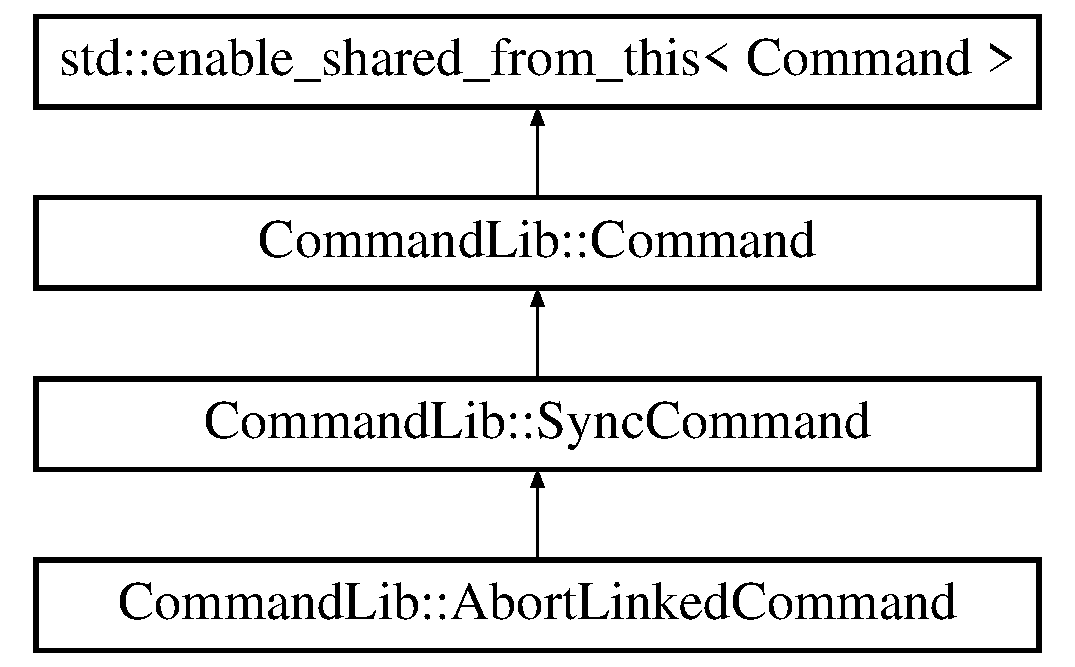
\includegraphics[height=4.000000cm]{class_command_lib_1_1_abort_linked_command}
\end{center}
\end{figure}
\subsection*{Public Types}
\begin{DoxyCompactItemize}
\item 
typedef std\+::shared\+\_\+ptr$<$ const \mbox{\hyperlink{class_command_lib_1_1_abort_linked_command}{Abort\+Linked\+Command}} $>$ \mbox{\hyperlink{class_command_lib_1_1_abort_linked_command_a45ac62243ddc4bff695a1abba7363dd8}{Const\+Ptr}}
\begin{DoxyCompactList}\small\item\em Shared pointer to a non-\/modifyable \mbox{\hyperlink{class_command_lib_1_1_abort_linked_command}{Abort\+Linked\+Command}} object\end{DoxyCompactList}\item 
typedef std\+::shared\+\_\+ptr$<$ \mbox{\hyperlink{class_command_lib_1_1_abort_linked_command}{Abort\+Linked\+Command}} $>$ \mbox{\hyperlink{class_command_lib_1_1_abort_linked_command_acb916ab386f796250b4978538d9eabd8}{Ptr}}
\begin{DoxyCompactList}\small\item\em Shared pointer to an \mbox{\hyperlink{class_command_lib_1_1_abort_linked_command}{Abort\+Linked\+Command}} object\end{DoxyCompactList}\end{DoxyCompactItemize}
\subsection*{Public Member Functions}
\begin{DoxyCompactItemize}
\item 
\mbox{\Hypertarget{class_command_lib_1_1_abort_linked_command_a014c2c8177e18e27f651aa122b58c90e}\label{class_command_lib_1_1_abort_linked_command_a014c2c8177e18e27f651aa122b58c90e}} 
virtual std\+::string \mbox{\hyperlink{class_command_lib_1_1_abort_linked_command_a014c2c8177e18e27f651aa122b58c90e}{Class\+Name}} () const override
\begin{DoxyCompactList}\small\item\em Gets the name of the runtime instance of this class. Used for logging and diagnostic purposes.  \end{DoxyCompactList}\item 
const \mbox{\hyperlink{class_command_lib_1_1_command_aee8fd78ff853a1f9c8e56959c3e81811}{Command\+::\+Const\+Ptr}} \mbox{\hyperlink{class_command_lib_1_1_abort_linked_command_ab61bc8cebde56e75016aa5bcea1ac175}{Command\+To\+Watch}} () const
\begin{DoxyCompactList}\small\item\em The command that will be monitored for abort events\end{DoxyCompactList}\end{DoxyCompactItemize}
\subsection*{Static Public Member Functions}
\begin{DoxyCompactItemize}
\item 
static \mbox{\hyperlink{class_command_lib_1_1_abort_linked_command_acb916ab386f796250b4978538d9eabd8}{Ptr}} \mbox{\hyperlink{class_command_lib_1_1_abort_linked_command_ab359541aab47533699365c2d74af1c5c}{Create}} (\mbox{\hyperlink{class_command_lib_1_1_command_a3b3e4f00144373299df5c6bb1acc319d}{Command\+::\+Ptr}} command\+To\+Run, \mbox{\hyperlink{class_command_lib_1_1_waitable_ac74b6b91e48220146eada76a31cf2d9b}{Waitable\+::\+Ptr}} abort\+Signal)
\begin{DoxyCompactList}\small\item\em Creates an \mbox{\hyperlink{class_command_lib_1_1_abort_linked_command}{Abort\+Linked\+Command}} object as a top-\/level \mbox{\hyperlink{class_command_lib_1_1_command}{Command}} \end{DoxyCompactList}\item 
static \mbox{\hyperlink{class_command_lib_1_1_abort_linked_command_acb916ab386f796250b4978538d9eabd8}{Ptr}} \mbox{\hyperlink{class_command_lib_1_1_abort_linked_command_ab3f6ae763ac98e85ce485d1cb7286960}{Create}} (\mbox{\hyperlink{class_command_lib_1_1_command_a3b3e4f00144373299df5c6bb1acc319d}{Command\+::\+Ptr}} command\+To\+Run, \mbox{\hyperlink{class_command_lib_1_1_command_aee8fd78ff853a1f9c8e56959c3e81811}{Command\+::\+Const\+Ptr}} command\+To\+Watch)
\begin{DoxyCompactList}\small\item\em Constructs an \mbox{\hyperlink{class_command_lib_1_1_abort_linked_command}{Abort\+Linked\+Command}} object as a top-\/level \mbox{\hyperlink{class_command_lib_1_1_command}{Command}} \end{DoxyCompactList}\end{DoxyCompactItemize}
\subsection*{Protected Member Functions}
\begin{DoxyCompactItemize}
\item 
\mbox{\hyperlink{class_command_lib_1_1_abort_linked_command_a0141b7dda2d5927ea405c888876224ec}{Abort\+Linked\+Command}} (\mbox{\hyperlink{class_command_lib_1_1_command_a3b3e4f00144373299df5c6bb1acc319d}{Command\+::\+Ptr}} command\+To\+Run, \mbox{\hyperlink{class_command_lib_1_1_waitable_ac74b6b91e48220146eada76a31cf2d9b}{Waitable\+::\+Ptr}} abort\+Event, \mbox{\hyperlink{class_command_lib_1_1_command_aee8fd78ff853a1f9c8e56959c3e81811}{Command\+::\+Const\+Ptr}} command\+To\+Watch)
\begin{DoxyCompactList}\small\item\em This constructor is not public so as to enforce creation using the \mbox{\hyperlink{class_command_lib_1_1_abort_linked_command_ab359541aab47533699365c2d74af1c5c}{Create()}} methods. \end{DoxyCompactList}\end{DoxyCompactItemize}
\subsection*{Additional Inherited Members}


\subsection{Detailed Description}
A \mbox{\hyperlink{class_command_lib_1_1_command}{Command}} wrapper that, in addition to responding to normal \mbox{\hyperlink{class_command_lib_1_1_command_a247cbc7325e3b9d9d7044d449b989aa6}{Command\+::\+Abort}} requests, also aborts in response to either 1) a request to abort a different, specified \mbox{\hyperlink{class_command_lib_1_1_command}{Command}} instance, or 2) the signaling of a specified \mbox{\hyperlink{class_command_lib_1_1_waitable}{Waitable}} (typically an \mbox{\hyperlink{class_command_lib_1_1_event}{Event}}). 

\mbox{\hyperlink{class_command_lib_1_1_abort_linked_command}{Abort\+Linked\+Command}} objects must be top level. Any attempt by another \mbox{\hyperlink{class_command_lib_1_1_command}{Command}} to take ownership of an \mbox{\hyperlink{class_command_lib_1_1_abort_linked_command}{Abort\+Linked\+Command}} will raise an exception. For example, adding this type to a \mbox{\hyperlink{class_command_lib_1_1_sequential_commands}{Sequential\+Commands}} will raise an exception because \mbox{\hyperlink{class_command_lib_1_1_sequential_commands}{Sequential\+Commands}} would attempt to assume ownership. 

\subsection{Member Typedef Documentation}
\mbox{\Hypertarget{class_command_lib_1_1_abort_linked_command_a45ac62243ddc4bff695a1abba7363dd8}\label{class_command_lib_1_1_abort_linked_command_a45ac62243ddc4bff695a1abba7363dd8}} 
\index{Command\+Lib\+::\+Abort\+Linked\+Command@{Command\+Lib\+::\+Abort\+Linked\+Command}!Const\+Ptr@{Const\+Ptr}}
\index{Const\+Ptr@{Const\+Ptr}!Command\+Lib\+::\+Abort\+Linked\+Command@{Command\+Lib\+::\+Abort\+Linked\+Command}}
\subsubsection{\texorpdfstring{Const\+Ptr}{ConstPtr}}
{\footnotesize\ttfamily typedef std\+::shared\+\_\+ptr$<$const \mbox{\hyperlink{class_command_lib_1_1_abort_linked_command}{Abort\+Linked\+Command}}$>$ \mbox{\hyperlink{class_command_lib_1_1_abort_linked_command_a45ac62243ddc4bff695a1abba7363dd8}{Command\+Lib\+::\+Abort\+Linked\+Command\+::\+Const\+Ptr}}}



Shared pointer to a non-\/modifyable \mbox{\hyperlink{class_command_lib_1_1_abort_linked_command}{Abort\+Linked\+Command}} object

\mbox{\Hypertarget{class_command_lib_1_1_abort_linked_command_acb916ab386f796250b4978538d9eabd8}\label{class_command_lib_1_1_abort_linked_command_acb916ab386f796250b4978538d9eabd8}} 
\index{Command\+Lib\+::\+Abort\+Linked\+Command@{Command\+Lib\+::\+Abort\+Linked\+Command}!Ptr@{Ptr}}
\index{Ptr@{Ptr}!Command\+Lib\+::\+Abort\+Linked\+Command@{Command\+Lib\+::\+Abort\+Linked\+Command}}
\subsubsection{\texorpdfstring{Ptr}{Ptr}}
{\footnotesize\ttfamily typedef std\+::shared\+\_\+ptr$<$\mbox{\hyperlink{class_command_lib_1_1_abort_linked_command}{Abort\+Linked\+Command}}$>$ \mbox{\hyperlink{class_command_lib_1_1_abort_linked_command_acb916ab386f796250b4978538d9eabd8}{Command\+Lib\+::\+Abort\+Linked\+Command\+::\+Ptr}}}



Shared pointer to an \mbox{\hyperlink{class_command_lib_1_1_abort_linked_command}{Abort\+Linked\+Command}} object



\subsection{Constructor \& Destructor Documentation}
\mbox{\Hypertarget{class_command_lib_1_1_abort_linked_command_a0141b7dda2d5927ea405c888876224ec}\label{class_command_lib_1_1_abort_linked_command_a0141b7dda2d5927ea405c888876224ec}} 
\index{Command\+Lib\+::\+Abort\+Linked\+Command@{Command\+Lib\+::\+Abort\+Linked\+Command}!Abort\+Linked\+Command@{Abort\+Linked\+Command}}
\index{Abort\+Linked\+Command@{Abort\+Linked\+Command}!Command\+Lib\+::\+Abort\+Linked\+Command@{Command\+Lib\+::\+Abort\+Linked\+Command}}
\subsubsection{\texorpdfstring{Abort\+Linked\+Command()}{AbortLinkedCommand()}}
{\footnotesize\ttfamily Command\+Lib\+::\+Abort\+Linked\+Command\+::\+Abort\+Linked\+Command (\begin{DoxyParamCaption}\item[{\mbox{\hyperlink{class_command_lib_1_1_command_a3b3e4f00144373299df5c6bb1acc319d}{Command\+::\+Ptr}}}]{command\+To\+Run,  }\item[{\mbox{\hyperlink{class_command_lib_1_1_waitable_ac74b6b91e48220146eada76a31cf2d9b}{Waitable\+::\+Ptr}}}]{abort\+Event,  }\item[{\mbox{\hyperlink{class_command_lib_1_1_command_aee8fd78ff853a1f9c8e56959c3e81811}{Command\+::\+Const\+Ptr}}}]{command\+To\+Watch }\end{DoxyParamCaption})\hspace{0.3cm}{\ttfamily [protected]}}



This constructor is not public so as to enforce creation using the \mbox{\hyperlink{class_command_lib_1_1_abort_linked_command_ab359541aab47533699365c2d74af1c5c}{Create()}} methods. 



\subsection{Member Function Documentation}
\mbox{\Hypertarget{class_command_lib_1_1_abort_linked_command_ab61bc8cebde56e75016aa5bcea1ac175}\label{class_command_lib_1_1_abort_linked_command_ab61bc8cebde56e75016aa5bcea1ac175}} 
\index{Command\+Lib\+::\+Abort\+Linked\+Command@{Command\+Lib\+::\+Abort\+Linked\+Command}!Command\+To\+Watch@{Command\+To\+Watch}}
\index{Command\+To\+Watch@{Command\+To\+Watch}!Command\+Lib\+::\+Abort\+Linked\+Command@{Command\+Lib\+::\+Abort\+Linked\+Command}}
\subsubsection{\texorpdfstring{Command\+To\+Watch()}{CommandToWatch()}}
{\footnotesize\ttfamily const \mbox{\hyperlink{class_command_lib_1_1_command_aee8fd78ff853a1f9c8e56959c3e81811}{Command\+::\+Const\+Ptr}} Command\+Lib\+::\+Abort\+Linked\+Command\+::\+Command\+To\+Watch (\begin{DoxyParamCaption}{ }\end{DoxyParamCaption}) const}



The command that will be monitored for abort events

\begin{DoxyReturn}{Returns}
The same value that was passed to the overloaded form of Create. This may be null, if that Create method was not used
\end{DoxyReturn}
\mbox{\Hypertarget{class_command_lib_1_1_abort_linked_command_ab359541aab47533699365c2d74af1c5c}\label{class_command_lib_1_1_abort_linked_command_ab359541aab47533699365c2d74af1c5c}} 
\index{Command\+Lib\+::\+Abort\+Linked\+Command@{Command\+Lib\+::\+Abort\+Linked\+Command}!Create@{Create}}
\index{Create@{Create}!Command\+Lib\+::\+Abort\+Linked\+Command@{Command\+Lib\+::\+Abort\+Linked\+Command}}
\subsubsection{\texorpdfstring{Create()}{Create()}\hspace{0.1cm}{\footnotesize\ttfamily [1/2]}}
{\footnotesize\ttfamily static \mbox{\hyperlink{class_command_lib_1_1_abort_linked_command_acb916ab386f796250b4978538d9eabd8}{Ptr}} Command\+Lib\+::\+Abort\+Linked\+Command\+::\+Create (\begin{DoxyParamCaption}\item[{\mbox{\hyperlink{class_command_lib_1_1_command_a3b3e4f00144373299df5c6bb1acc319d}{Command\+::\+Ptr}}}]{command\+To\+Run,  }\item[{\mbox{\hyperlink{class_command_lib_1_1_waitable_ac74b6b91e48220146eada76a31cf2d9b}{Waitable\+::\+Ptr}}}]{abort\+Signal }\end{DoxyParamCaption})\hspace{0.3cm}{\ttfamily [static]}}



Creates an \mbox{\hyperlink{class_command_lib_1_1_abort_linked_command}{Abort\+Linked\+Command}} object as a top-\/level \mbox{\hyperlink{class_command_lib_1_1_command}{Command}} 


\begin{DoxyParams}{Parameters}
{\em command\+To\+Run} & The command to run. This object takes ownership of the command, so the passed command must not already have an owner. \\
\hline
{\em abort\+Signal} & When signaled, the command to run will be aborted. This object does not take ownership of this parameter. \\
\hline
\end{DoxyParams}
\mbox{\Hypertarget{class_command_lib_1_1_abort_linked_command_ab3f6ae763ac98e85ce485d1cb7286960}\label{class_command_lib_1_1_abort_linked_command_ab3f6ae763ac98e85ce485d1cb7286960}} 
\index{Command\+Lib\+::\+Abort\+Linked\+Command@{Command\+Lib\+::\+Abort\+Linked\+Command}!Create@{Create}}
\index{Create@{Create}!Command\+Lib\+::\+Abort\+Linked\+Command@{Command\+Lib\+::\+Abort\+Linked\+Command}}
\subsubsection{\texorpdfstring{Create()}{Create()}\hspace{0.1cm}{\footnotesize\ttfamily [2/2]}}
{\footnotesize\ttfamily static \mbox{\hyperlink{class_command_lib_1_1_abort_linked_command_acb916ab386f796250b4978538d9eabd8}{Ptr}} Command\+Lib\+::\+Abort\+Linked\+Command\+::\+Create (\begin{DoxyParamCaption}\item[{\mbox{\hyperlink{class_command_lib_1_1_command_a3b3e4f00144373299df5c6bb1acc319d}{Command\+::\+Ptr}}}]{command\+To\+Run,  }\item[{\mbox{\hyperlink{class_command_lib_1_1_command_aee8fd78ff853a1f9c8e56959c3e81811}{Command\+::\+Const\+Ptr}}}]{command\+To\+Watch }\end{DoxyParamCaption})\hspace{0.3cm}{\ttfamily [static]}}



Constructs an \mbox{\hyperlink{class_command_lib_1_1_abort_linked_command}{Abort\+Linked\+Command}} object as a top-\/level \mbox{\hyperlink{class_command_lib_1_1_command}{Command}} 


\begin{DoxyParams}{Parameters}
{\em command\+To\+Run} & The command to run. This object takes ownership of the command, so the passed command must not already have an owner. \\
\hline
{\em command\+To\+Watch} & When this \textquotesingle{}command\+To\+Watch\textquotesingle{} is aborted, the command to run will also be aborted. \\
\hline
\end{DoxyParams}


The documentation for this class was generated from the following file\+:\begin{DoxyCompactItemize}
\item 
C\+:/\+Users/efieleke/\+Documents/\+Git\+Hub/\+Command\+Lib\+For\+C\+P\+P/\+Command\+Lib/include/Abort\+Linked\+Command.\+h\end{DoxyCompactItemize}

\hypertarget{class_command_lib_1_1_async_command}{}\doxysection{Command\+Lib\+::Async\+Command Class Reference}
\label{class_command_lib_1_1_async_command}\index{CommandLib::AsyncCommand@{CommandLib::AsyncCommand}}


Represents a \mbox{\hyperlink{class_command_lib_1_1_command}{Command}} which is most naturally asynchronous in its implementation. If you inherit from this class, you are responsible for implementing Command\+::\+Async\+Execute\+Impl. This class implements Command\+::\+Sync\+Execute\+Impl.  




{\ttfamily \#include $<$Async\+Command.\+h$>$}

Inheritance diagram for Command\+Lib\+::Async\+Command\+:\begin{figure}[H]
\begin{center}
\leavevmode
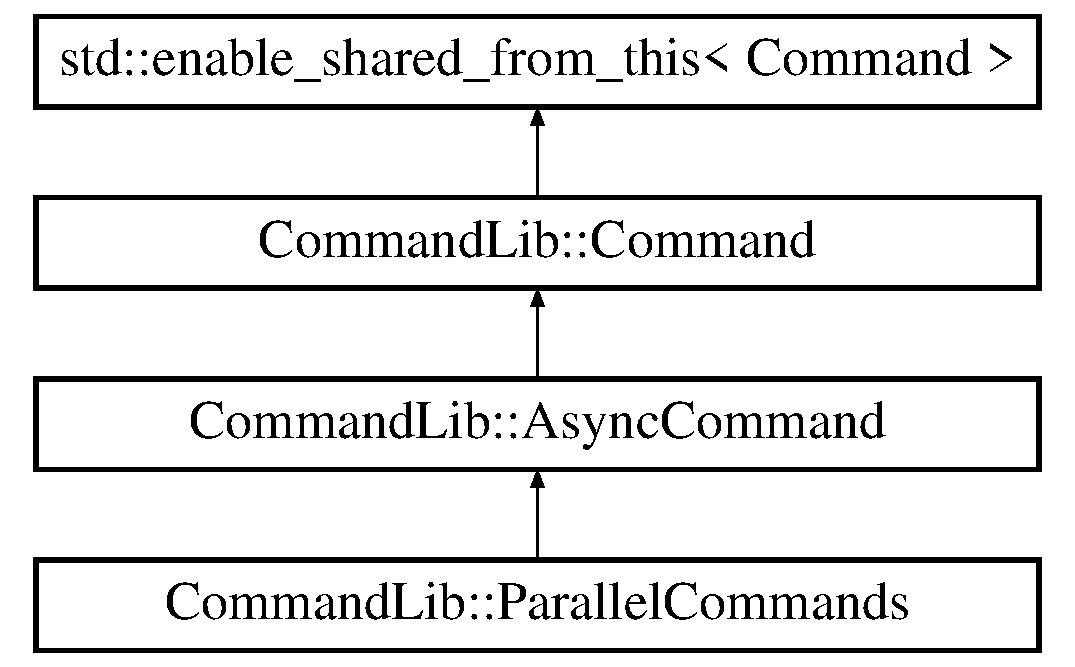
\includegraphics[height=4.000000cm]{class_command_lib_1_1_async_command}
\end{center}
\end{figure}
\doxysubsection*{Public Member Functions}
\begin{DoxyCompactItemize}
\item 
\mbox{\Hypertarget{class_command_lib_1_1_async_command_a2c08165637770cc7bb8fdd814a93acec}\label{class_command_lib_1_1_async_command_a2c08165637770cc7bb8fdd814a93acec}} 
virtual bool \mbox{\hyperlink{class_command_lib_1_1_async_command_a2c08165637770cc7bb8fdd814a93acec}{Is\+Naturally\+Synchronous}} () const final
\begin{DoxyCompactList}\small\item\em Returns true if this command\textquotesingle{}s most efficient form of execution is synchronous. This information is used on occasion to determine how to best execute a command. \end{DoxyCompactList}\end{DoxyCompactItemize}
\doxysubsection*{Additional Inherited Members}


\doxysubsection{Detailed Description}
Represents a \mbox{\hyperlink{class_command_lib_1_1_command}{Command}} which is most naturally asynchronous in its implementation. If you inherit from this class, you are responsible for implementing Command\+::\+Async\+Execute\+Impl. This class implements Command\+::\+Sync\+Execute\+Impl. 



The documentation for this class was generated from the following file\+:\begin{DoxyCompactItemize}
\item 
Command\+Lib\+For\+CPP/\+Command\+Lib/include/Async\+Command.\+h\end{DoxyCompactItemize}

\hypertarget{class_command_lib_1_1_command}{}\section{Command\+Lib\+:\+:Command Class Reference}
\label{class_command_lib_1_1_command}\index{Command\+Lib\+::\+Command@{Command\+Lib\+::\+Command}}


Represents an action that can be run synchronously or asynchronously. 




{\ttfamily \#include $<$Command.\+h$>$}

Inheritance diagram for Command\+Lib\+:\+:Command\+:\begin{figure}[H]
\begin{center}
\leavevmode
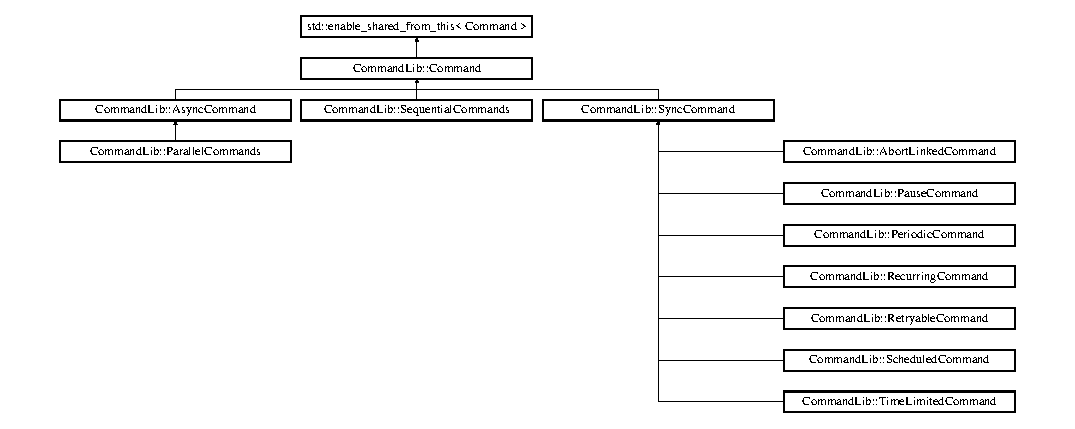
\includegraphics[height=5.323195cm]{class_command_lib_1_1_command}
\end{center}
\end{figure}
\subsection*{Public Types}
\begin{DoxyCompactItemize}
\item 
typedef std\+::shared\+\_\+ptr$<$ const \mbox{\hyperlink{class_command_lib_1_1_command}{Command}} $>$ \mbox{\hyperlink{class_command_lib_1_1_command_aee8fd78ff853a1f9c8e56959c3e81811}{Const\+Ptr}}
\begin{DoxyCompactList}\small\item\em Shared pointer to a non-\/modifyable \mbox{\hyperlink{class_command_lib_1_1_command}{Command}} object\end{DoxyCompactList}\item 
typedef std\+::shared\+\_\+ptr$<$ \mbox{\hyperlink{class_command_lib_1_1_command}{Command}} $>$ \mbox{\hyperlink{class_command_lib_1_1_command_a3b3e4f00144373299df5c6bb1acc319d}{Ptr}}
\begin{DoxyCompactList}\small\item\em Shared pointer to a \mbox{\hyperlink{class_command_lib_1_1_command}{Command}} object\end{DoxyCompactList}\end{DoxyCompactItemize}
\subsection*{Public Member Functions}
\begin{DoxyCompactItemize}
\item 
long \mbox{\hyperlink{class_command_lib_1_1_command_a00a3047609fda3d69b828b7850624389}{Id}} () const
\begin{DoxyCompactList}\small\item\em The unique identifier for this command\end{DoxyCompactList}\item 
const \mbox{\hyperlink{class_command_lib_1_1_command}{Command}} $\ast$ \mbox{\hyperlink{class_command_lib_1_1_command_a19a55aef338aad892fc105b2e1f8700f}{Parent}} () const
\begin{DoxyCompactList}\small\item\em The command under which this command is nested, if any\end{DoxyCompactList}\item 
int \mbox{\hyperlink{class_command_lib_1_1_command_a28e3c6c7f6467cbeffe287984c3f012d}{Depth}} () const
\begin{DoxyCompactList}\small\item\em How deeply nested this command is\end{DoxyCompactList}\item 
std\+::string \mbox{\hyperlink{class_command_lib_1_1_command_a03783e0aea82f820805b8c4e9cc8b43e}{Description}} () const
\begin{DoxyCompactList}\small\item\em A description of the \mbox{\hyperlink{class_command_lib_1_1_command}{Command}}\end{DoxyCompactList}\item 
virtual std\+::string \mbox{\hyperlink{class_command_lib_1_1_command_a795a185509e7b0fc1606b3b62fe17fbb}{Extended\+Description}} () const
\begin{DoxyCompactList}\small\item\em Information about the command (beyond its type and id), if available, for diagnostic purposes. \end{DoxyCompactList}\item 
virtual bool \mbox{\hyperlink{class_command_lib_1_1_command_a4ccad987c43709c44c20132c3890b585}{Is\+Naturally\+Synchronous}} () const =0
\begin{DoxyCompactList}\small\item\em Returns true if this command\textquotesingle{}s most efficient form of execution is synchronous. This information is used on occasion to determine how to best execute a command. \end{DoxyCompactList}\item 
void \mbox{\hyperlink{class_command_lib_1_1_command_a5d33760ccb927d7f6349c02907ab4ff3}{Sync\+Execute}} ()
\begin{DoxyCompactList}\small\item\em Executes the command and does not return until it finishes.\end{DoxyCompactList}\item 
void \mbox{\hyperlink{class_command_lib_1_1_command_a663d50889f527a4963eebd88bbcdc522}{Sync\+Execute}} (\mbox{\hyperlink{class_command_lib_1_1_command}{Command}} $\ast$owner)
\begin{DoxyCompactList}\small\item\em Executes the command and does not return until it finishes.\end{DoxyCompactList}\item 
void \mbox{\hyperlink{class_command_lib_1_1_command_a44bad231a0f0a6de3d5405382d95f800}{Async\+Execute}} (\mbox{\hyperlink{class_command_lib_1_1_command_listener}{Command\+Listener}} $\ast$listener)
\begin{DoxyCompactList}\small\item\em Starts executing the command and returns immediately. \end{DoxyCompactList}\item 
void \mbox{\hyperlink{class_command_lib_1_1_command_a247cbc7325e3b9d9d7044d449b989aa6}{Abort}} ()
\begin{DoxyCompactList}\small\item\em Aborts a running command\end{DoxyCompactList}\item 
void \mbox{\hyperlink{class_command_lib_1_1_command_ac4d49fbf9bbcc543fb57e4b04edf1ddb}{Wait}} () const
\begin{DoxyCompactList}\small\item\em Waits for a running command to complete. Will return immediately if the command is not currently executing. \end{DoxyCompactList}\item 
{\footnotesize template$<$typename Rep , typename Period $>$ }\\bool \mbox{\hyperlink{class_command_lib_1_1_command_a0cd3c0e7ee280652c69a3e13a30b99e7}{Wait}} (const std\+::chrono\+::duration$<$ Rep, Period $>$ \&interval) const
\begin{DoxyCompactList}\small\item\em Waits a specified duration for a running command to complete. Will return immediately if the command is not currently executing. \end{DoxyCompactList}\item 
bool \mbox{\hyperlink{class_command_lib_1_1_command_ad4cae3ab883426e4f872782b8de88597}{Wait}} (long long milliseconds) const
\begin{DoxyCompactList}\small\item\em Waits the specified milliseconds for a running command to complete. Will return immediately if the command is not currently executing. \end{DoxyCompactList}\item 
void \mbox{\hyperlink{class_command_lib_1_1_command_a6afa9e7eab83d5e59746fe15e295e066}{Abort\+And\+Wait}} ()
\begin{DoxyCompactList}\small\item\em The exact same effect as a call to \mbox{\hyperlink{class_command_lib_1_1_command_a247cbc7325e3b9d9d7044d449b989aa6}{Abort}} immediately followed by a call to \mbox{\hyperlink{class_command_lib_1_1_command_ac4d49fbf9bbcc543fb57e4b04edf1ddb}{Wait}} \end{DoxyCompactList}\item 
{\footnotesize template$<$typename Rep , typename Period $>$ }\\bool \mbox{\hyperlink{class_command_lib_1_1_command_af51df64ba29324bbbbe13c647e708563}{Abort\+And\+Wait}} (const std\+::chrono\+::duration$<$ Rep, Period $>$ \&interval) const
\begin{DoxyCompactList}\small\item\em The exact same effect as a call to \mbox{\hyperlink{class_command_lib_1_1_command_a247cbc7325e3b9d9d7044d449b989aa6}{Abort}} immediately followed by a call to Wait(const std\+::chrono\+::duration$<$\+Rep, Period$>$\&) \end{DoxyCompactList}\item 
bool \mbox{\hyperlink{class_command_lib_1_1_command_ab7e0fd4eb4f1d2b6d98228c1432805e3}{Abort\+And\+Wait}} (long long milliseconds)
\begin{DoxyCompactList}\small\item\em The exact same effect as a call to \mbox{\hyperlink{class_command_lib_1_1_command_a247cbc7325e3b9d9d7044d449b989aa6}{Abort}} immediately followed by a call to Wait(const std\+::chrono\+::duration$<$\+Rep, Period$>$\&) \end{DoxyCompactList}\item 
virtual std\+::string \mbox{\hyperlink{class_command_lib_1_1_command_a96f8ac531b436a41b21252fa2e17fd79}{Class\+Name}} () const =0
\begin{DoxyCompactList}\small\item\em Gets the name of the runtime instance of this class. Used for logging and diagnostic purposes. \end{DoxyCompactList}\item 
\mbox{\hyperlink{class_command_lib_1_1_waitable_ac74b6b91e48220146eada76a31cf2d9b}{Waitable\+::\+Ptr}} \mbox{\hyperlink{class_command_lib_1_1_command_a5f163dafd55fe63a5ed351e1543d02a3}{Done\+Event}} () const
\begin{DoxyCompactList}\small\item\em Signaled when this command has finished execution, regardless of whether it succeeded, failed or was aborted. \end{DoxyCompactList}\item 
\mbox{\hyperlink{class_command_lib_1_1_waitable_ac74b6b91e48220146eada76a31cf2d9b}{Waitable\+::\+Ptr}} \mbox{\hyperlink{class_command_lib_1_1_command_a1fdc8e982866dbbfb763af5d755f76dd}{Abort\+Event}} () const
\begin{DoxyCompactList}\small\item\em Signaled when this command is to be aborted. Note that this event is only reset when the command next begins execution. \end{DoxyCompactList}\end{DoxyCompactItemize}
\subsection*{Static Public Attributes}
\begin{DoxyCompactItemize}
\item 
static std\+::list$<$ \mbox{\hyperlink{class_command_lib_1_1_command_monitor}{Command\+Monitor}} $\ast$ $>$ \mbox{\hyperlink{class_command_lib_1_1_command_aa4ceb8d85a720bc5d9bac4be3afd7df5}{sm\+\_\+monitors}}
\begin{DoxyCompactList}\small\item\em The objects that define command monitoring behavior. Monitoring is meant for logging and diagnostic purposes. \end{DoxyCompactList}\end{DoxyCompactItemize}
\subsection*{Protected Member Functions}
\begin{DoxyCompactItemize}
\item 
\mbox{\hyperlink{class_command_lib_1_1_command_a31713edf2ee9c217f9090e5337dd1f44}{Command}} ()
\begin{DoxyCompactList}\small\item\em Constructor \end{DoxyCompactList}\item 
void \mbox{\hyperlink{class_command_lib_1_1_command_a0787e7b79c5424926be5c1c8be1ebb0d}{Take\+Ownership}} (\mbox{\hyperlink{class_command_lib_1_1_command_a3b3e4f00144373299df5c6bb1acc319d}{Ptr}} orphan)
\begin{DoxyCompactList}\small\item\em Make this command the owner of the command passed as an argument.\end{DoxyCompactList}\item 
void \mbox{\hyperlink{class_command_lib_1_1_command_ac872e76c74ed573668b60351fd9ffd1d}{Relinquish\+Ownership}} (\mbox{\hyperlink{class_command_lib_1_1_command_a3b3e4f00144373299df5c6bb1acc319d}{Ptr}} command)
\begin{DoxyCompactList}\small\item\em Makes what used to be an owned command a top-\/level command.\end{DoxyCompactList}\item 
void \mbox{\hyperlink{class_command_lib_1_1_command_a0e9fe77b6976159e86428ebcaeee0e82}{Check\+Abort\+Flag}} () const
\begin{DoxyCompactList}\small\item\em Throws a \mbox{\hyperlink{class_command_lib_1_1_command_aborted_exception}{Command\+Aborted\+Exception}} if an abort is pending. Synchronous implementations may find this useful in order to respond to an abort request in a timely manner. \end{DoxyCompactList}\end{DoxyCompactItemize}
\subsection*{Friends}
\begin{DoxyCompactItemize}
\item 
\mbox{\Hypertarget{class_command_lib_1_1_command_abff6f12669682d683b4c150859ce09fc}\label{class_command_lib_1_1_command_abff6f12669682d683b4c150859ce09fc}} 
class {\bfseries Async\+Command}
\end{DoxyCompactItemize}


\subsection{Detailed Description}
Represents an action that can be run synchronously or asynchronously.

Commands are abortable. Even a synchronously running command can be aborted from a separate thread. 

\mbox{\hyperlink{class_command_lib_1_1_command}{Command}} types are only instantiable via static Create() methods. This is because commands often own other commands. It was necessary to either enforce clone interface support, or enforce working with smart pointers. Smart pointers felt like the easier approach for clients (writing clone methods is a nuisance). 

When developing a \mbox{\hyperlink{class_command_lib_1_1_command}{Command}} subclass, be sure to inherit from either \mbox{\hyperlink{class_command_lib_1_1_sync_command}{Sync\+Command}} (if your command is naturally synchronous in its implementation) or \mbox{\hyperlink{class_command_lib_1_1_async_command}{Async\+Command}}. Those classes take care of the unnatural implementations (\mbox{\hyperlink{class_command_lib_1_1_sync_command}{Sync\+Command}} implements Async\+Execute\+Impl, and \mbox{\hyperlink{class_command_lib_1_1_async_command}{Async\+Command}} implements Sync\+Execute\+Impl). 

Also, when developing a \mbox{\hyperlink{class_command_lib_1_1_command}{Command}} subclass, make sure that any member variables that are Commands are properly owned by calling \mbox{\hyperlink{class_command_lib_1_1_command_a0787e7b79c5424926be5c1c8be1ebb0d}{Take\+Ownership}} within your constructor body. The advantage of doing this is that owned commands will automatically respond to abort requests issued to the owner. 

If you write a method that accepts a \mbox{\hyperlink{class_command_lib_1_1_command}{Command}} as an argument, you may wish to assume ownership of that \mbox{\hyperlink{class_command_lib_1_1_command}{Command}}. \mbox{\hyperlink{class_command_lib_1_1_command_a0787e7b79c5424926be5c1c8be1ebb0d}{Take\+Ownership}} allows you to do this. The \mbox{\hyperlink{class_command_lib_1_1_sequential_commands_af0100e15f7897471ce84802ab6c25e00}{Sequential\+Commands\+::\+Add}} member of \mbox{\hyperlink{class_command_lib_1_1_sequential_commands}{Sequential\+Commands}} is an example of this behavior. 

If you find that you need to create a \mbox{\hyperlink{class_command_lib_1_1_command}{Command}} object within the execution method of its owning command (perhaps because which type of \mbox{\hyperlink{class_command_lib_1_1_command}{Command}} to create depends upon runtime conditions), there are some things to consider. Owned commands are not destroyed until the owner is destroyed. If the owner is executed many times before it is destroyed, and you create a new child command upon every execution, resource usage will grow unbounded. The better approach is not assign an owner to the locally created command, but instead have it run within the context of the launching command using \mbox{\hyperlink{class_command_lib_1_1_command_a663d50889f527a4963eebd88bbcdc522}{Sync\+Execute(\+Command$\ast$)}}. If you require asynchronous execution, you can make use of \mbox{\hyperlink{class_command_lib_1_1_abort_linked_command}{Abort\+Linked\+Command}}. This will return a top-\/level command that responds to abort requests to the command that created it. 

Generally speaking, when authoring Commands, it\textquotesingle{}s best to make them as granular as possible. That makes it much easier to reuse them while composing command structures. Also, ensure that your commands are responsive to abort requests if they take a noticeable amount of time to complete. 

\subsection{Member Typedef Documentation}
\mbox{\Hypertarget{class_command_lib_1_1_command_aee8fd78ff853a1f9c8e56959c3e81811}\label{class_command_lib_1_1_command_aee8fd78ff853a1f9c8e56959c3e81811}} 
\index{Command\+Lib\+::\+Command@{Command\+Lib\+::\+Command}!Const\+Ptr@{Const\+Ptr}}
\index{Const\+Ptr@{Const\+Ptr}!Command\+Lib\+::\+Command@{Command\+Lib\+::\+Command}}
\subsubsection{\texorpdfstring{Const\+Ptr}{ConstPtr}}
{\footnotesize\ttfamily typedef std\+::shared\+\_\+ptr$<$const \mbox{\hyperlink{class_command_lib_1_1_command}{Command}}$>$ \mbox{\hyperlink{class_command_lib_1_1_command_aee8fd78ff853a1f9c8e56959c3e81811}{Command\+Lib\+::\+Command\+::\+Const\+Ptr}}}



Shared pointer to a non-\/modifyable \mbox{\hyperlink{class_command_lib_1_1_command}{Command}} object

\mbox{\Hypertarget{class_command_lib_1_1_command_a3b3e4f00144373299df5c6bb1acc319d}\label{class_command_lib_1_1_command_a3b3e4f00144373299df5c6bb1acc319d}} 
\index{Command\+Lib\+::\+Command@{Command\+Lib\+::\+Command}!Ptr@{Ptr}}
\index{Ptr@{Ptr}!Command\+Lib\+::\+Command@{Command\+Lib\+::\+Command}}
\subsubsection{\texorpdfstring{Ptr}{Ptr}}
{\footnotesize\ttfamily typedef std\+::shared\+\_\+ptr$<$\mbox{\hyperlink{class_command_lib_1_1_command}{Command}}$>$ \mbox{\hyperlink{class_command_lib_1_1_command_a3b3e4f00144373299df5c6bb1acc319d}{Command\+Lib\+::\+Command\+::\+Ptr}}}



Shared pointer to a \mbox{\hyperlink{class_command_lib_1_1_command}{Command}} object



\subsection{Constructor \& Destructor Documentation}
\mbox{\Hypertarget{class_command_lib_1_1_command_a31713edf2ee9c217f9090e5337dd1f44}\label{class_command_lib_1_1_command_a31713edf2ee9c217f9090e5337dd1f44}} 
\index{Command\+Lib\+::\+Command@{Command\+Lib\+::\+Command}!Command@{Command}}
\index{Command@{Command}!Command\+Lib\+::\+Command@{Command\+Lib\+::\+Command}}
\subsubsection{\texorpdfstring{Command()}{Command()}}
{\footnotesize\ttfamily Command\+Lib\+::\+Command\+::\+Command (\begin{DoxyParamCaption}{ }\end{DoxyParamCaption})\hspace{0.3cm}{\ttfamily [protected]}}



Constructor 



\subsection{Member Function Documentation}
\mbox{\Hypertarget{class_command_lib_1_1_command_a247cbc7325e3b9d9d7044d449b989aa6}\label{class_command_lib_1_1_command_a247cbc7325e3b9d9d7044d449b989aa6}} 
\index{Command\+Lib\+::\+Command@{Command\+Lib\+::\+Command}!Abort@{Abort}}
\index{Abort@{Abort}!Command\+Lib\+::\+Command@{Command\+Lib\+::\+Command}}
\subsubsection{\texorpdfstring{Abort()}{Abort()}}
{\footnotesize\ttfamily void Command\+Lib\+::\+Command\+::\+Abort (\begin{DoxyParamCaption}{ }\end{DoxyParamCaption})}



Aborts a running command

This method will have no effect on a command that is not running (nor will it cause a future execution of this command to abort). Synchronous execution will throw a \mbox{\hyperlink{class_command_lib_1_1_command_aborted_exception}{Command\+Aborted\+Exception}} if aborted, and asynchronous execution will invoke \mbox{\hyperlink{class_command_lib_1_1_command_listener_aa389ff6dd3895ce4ecc9447a23e4d9fc}{Command\+Listener\+::\+Command\+Aborted}} on the listener if aborted. Note that if a command is near completion, it may finish successfully (or fail) before an abort request is processed. 

It is an error to call \mbox{\hyperlink{class_command_lib_1_1_command_a247cbc7325e3b9d9d7044d449b989aa6}{Abort()}} on anything other than a top level command. \mbox{\Hypertarget{class_command_lib_1_1_command_a6afa9e7eab83d5e59746fe15e295e066}\label{class_command_lib_1_1_command_a6afa9e7eab83d5e59746fe15e295e066}} 
\index{Command\+Lib\+::\+Command@{Command\+Lib\+::\+Command}!Abort\+And\+Wait@{Abort\+And\+Wait}}
\index{Abort\+And\+Wait@{Abort\+And\+Wait}!Command\+Lib\+::\+Command@{Command\+Lib\+::\+Command}}
\subsubsection{\texorpdfstring{Abort\+And\+Wait()}{AbortAndWait()}\hspace{0.1cm}{\footnotesize\ttfamily [1/3]}}
{\footnotesize\ttfamily void Command\+Lib\+::\+Command\+::\+Abort\+And\+Wait (\begin{DoxyParamCaption}{ }\end{DoxyParamCaption})}



The exact same effect as a call to \mbox{\hyperlink{class_command_lib_1_1_command_a247cbc7325e3b9d9d7044d449b989aa6}{Abort}} immediately followed by a call to \mbox{\hyperlink{class_command_lib_1_1_command_ac4d49fbf9bbcc543fb57e4b04edf1ddb}{Wait}} 

\mbox{\Hypertarget{class_command_lib_1_1_command_af51df64ba29324bbbbe13c647e708563}\label{class_command_lib_1_1_command_af51df64ba29324bbbbe13c647e708563}} 
\index{Command\+Lib\+::\+Command@{Command\+Lib\+::\+Command}!Abort\+And\+Wait@{Abort\+And\+Wait}}
\index{Abort\+And\+Wait@{Abort\+And\+Wait}!Command\+Lib\+::\+Command@{Command\+Lib\+::\+Command}}
\subsubsection{\texorpdfstring{Abort\+And\+Wait()}{AbortAndWait()}\hspace{0.1cm}{\footnotesize\ttfamily [2/3]}}
{\footnotesize\ttfamily template$<$typename Rep , typename Period $>$ \\
bool Command\+Lib\+::\+Command\+::\+Abort\+And\+Wait (\begin{DoxyParamCaption}\item[{const std\+::chrono\+::duration$<$ Rep, Period $>$ \&}]{interval }\end{DoxyParamCaption}) const\hspace{0.3cm}{\ttfamily [inline]}}



The exact same effect as a call to \mbox{\hyperlink{class_command_lib_1_1_command_a247cbc7325e3b9d9d7044d449b989aa6}{Abort}} immediately followed by a call to Wait(const std\+::chrono\+::duration$<$\+Rep, Period$>$\&) 


\begin{DoxyParams}{Parameters}
{\em interval} & The maximum amount of time to wait\\
\hline
\end{DoxyParams}
\begin{DoxyReturn}{Returns}
true if the the command completed within \textquotesingle{}duration\textquotesingle{}, false otherwise
\end{DoxyReturn}
\mbox{\Hypertarget{class_command_lib_1_1_command_ab7e0fd4eb4f1d2b6d98228c1432805e3}\label{class_command_lib_1_1_command_ab7e0fd4eb4f1d2b6d98228c1432805e3}} 
\index{Command\+Lib\+::\+Command@{Command\+Lib\+::\+Command}!Abort\+And\+Wait@{Abort\+And\+Wait}}
\index{Abort\+And\+Wait@{Abort\+And\+Wait}!Command\+Lib\+::\+Command@{Command\+Lib\+::\+Command}}
\subsubsection{\texorpdfstring{Abort\+And\+Wait()}{AbortAndWait()}\hspace{0.1cm}{\footnotesize\ttfamily [3/3]}}
{\footnotesize\ttfamily bool Command\+Lib\+::\+Command\+::\+Abort\+And\+Wait (\begin{DoxyParamCaption}\item[{long long}]{milliseconds }\end{DoxyParamCaption})}



The exact same effect as a call to \mbox{\hyperlink{class_command_lib_1_1_command_a247cbc7325e3b9d9d7044d449b989aa6}{Abort}} immediately followed by a call to Wait(const std\+::chrono\+::duration$<$\+Rep, Period$>$\&) 


\begin{DoxyParams}{Parameters}
{\em milliseconds} & The maximum number of milliseconds to wait\\
\hline
\end{DoxyParams}
\begin{DoxyReturn}{Returns}
true if the the command completed within \textquotesingle{}duration\textquotesingle{}, false otherwise
\end{DoxyReturn}
\mbox{\Hypertarget{class_command_lib_1_1_command_a1fdc8e982866dbbfb763af5d755f76dd}\label{class_command_lib_1_1_command_a1fdc8e982866dbbfb763af5d755f76dd}} 
\index{Command\+Lib\+::\+Command@{Command\+Lib\+::\+Command}!Abort\+Event@{Abort\+Event}}
\index{Abort\+Event@{Abort\+Event}!Command\+Lib\+::\+Command@{Command\+Lib\+::\+Command}}
\subsubsection{\texorpdfstring{Abort\+Event()}{AbortEvent()}}
{\footnotesize\ttfamily \mbox{\hyperlink{class_command_lib_1_1_waitable_ac74b6b91e48220146eada76a31cf2d9b}{Waitable\+::\+Ptr}} Command\+Lib\+::\+Command\+::\+Abort\+Event (\begin{DoxyParamCaption}{ }\end{DoxyParamCaption}) const}



Signaled when this command is to be aborted. Note that this event is only reset when the command next begins execution. 

\begin{DoxyReturn}{Returns}
The object that can waited up for this command to be signaled to abort.
\end{DoxyReturn}


Note that this is signaled when the command should abort, which will be before the command finishes aborting itself\mbox{\Hypertarget{class_command_lib_1_1_command_a44bad231a0f0a6de3d5405382d95f800}\label{class_command_lib_1_1_command_a44bad231a0f0a6de3d5405382d95f800}} 
\index{Command\+Lib\+::\+Command@{Command\+Lib\+::\+Command}!Async\+Execute@{Async\+Execute}}
\index{Async\+Execute@{Async\+Execute}!Command\+Lib\+::\+Command@{Command\+Lib\+::\+Command}}
\subsubsection{\texorpdfstring{Async\+Execute()}{AsyncExecute()}}
{\footnotesize\ttfamily void Command\+Lib\+::\+Command\+::\+Async\+Execute (\begin{DoxyParamCaption}\item[{\mbox{\hyperlink{class_command_lib_1_1_command_listener}{Command\+Listener}} $\ast$}]{listener }\end{DoxyParamCaption})}



Starts executing the command and returns immediately. 

Call \mbox{\hyperlink{class_command_lib_1_1_command_ac4d49fbf9bbcc543fb57e4b04edf1ddb}{Wait}} if you need to block until the command finishes. 

It is safe to call this any number of times, but it will cause undefined behavior to re-\/execute a command that is already executing. 


\begin{DoxyParams}{Parameters}
{\em listener} & One of the methods of this interface will be called upon completion, on a separate thread. See the \mbox{\hyperlink{class_command_lib_1_1_command_listener}{Command\+Listener}} documentation for details. \\
\hline
\end{DoxyParams}
\mbox{\Hypertarget{class_command_lib_1_1_command_a0e9fe77b6976159e86428ebcaeee0e82}\label{class_command_lib_1_1_command_a0e9fe77b6976159e86428ebcaeee0e82}} 
\index{Command\+Lib\+::\+Command@{Command\+Lib\+::\+Command}!Check\+Abort\+Flag@{Check\+Abort\+Flag}}
\index{Check\+Abort\+Flag@{Check\+Abort\+Flag}!Command\+Lib\+::\+Command@{Command\+Lib\+::\+Command}}
\subsubsection{\texorpdfstring{Check\+Abort\+Flag()}{CheckAbortFlag()}}
{\footnotesize\ttfamily void Command\+Lib\+::\+Command\+::\+Check\+Abort\+Flag (\begin{DoxyParamCaption}{ }\end{DoxyParamCaption}) const\hspace{0.3cm}{\ttfamily [protected]}}



Throws a \mbox{\hyperlink{class_command_lib_1_1_command_aborted_exception}{Command\+Aborted\+Exception}} if an abort is pending. Synchronous implementations may find this useful in order to respond to an abort request in a timely manner. 

\mbox{\Hypertarget{class_command_lib_1_1_command_a96f8ac531b436a41b21252fa2e17fd79}\label{class_command_lib_1_1_command_a96f8ac531b436a41b21252fa2e17fd79}} 
\index{Command\+Lib\+::\+Command@{Command\+Lib\+::\+Command}!Class\+Name@{Class\+Name}}
\index{Class\+Name@{Class\+Name}!Command\+Lib\+::\+Command@{Command\+Lib\+::\+Command}}
\subsubsection{\texorpdfstring{Class\+Name()}{ClassName()}}
{\footnotesize\ttfamily virtual std\+::string Command\+Lib\+::\+Command\+::\+Class\+Name (\begin{DoxyParamCaption}{ }\end{DoxyParamCaption}) const\hspace{0.3cm}{\ttfamily [pure virtual]}}



Gets the name of the runtime instance of this class. Used for logging and diagnostic purposes. 

The returned string should be the name of the derived class, without any namespace qualification. I could have used typeid instead, but that requires compiling with R\+T\+TI, which is not something that everyone wants. 

Implemented in \mbox{\hyperlink{class_command_lib_1_1_periodic_command_a77c34a0f31ae4e7f0c642a356bd5d6ef}{Command\+Lib\+::\+Periodic\+Command}}, \mbox{\hyperlink{class_command_lib_1_1_pause_command_afcdddf1fa8b52a3bfec665b1db736cc5}{Command\+Lib\+::\+Pause\+Command}}, \mbox{\hyperlink{class_command_lib_1_1_recurring_command_a4e2073b92185dd5f7b545d774afbb929}{Command\+Lib\+::\+Recurring\+Command}}, \mbox{\hyperlink{class_command_lib_1_1_scheduled_command_ae01bdda88e63460a380579e08ced9eda}{Command\+Lib\+::\+Scheduled\+Command}}, \mbox{\hyperlink{class_command_lib_1_1_time_limited_command_a2a5063ef124f555229b90f7bd82f362e}{Command\+Lib\+::\+Time\+Limited\+Command}}, \mbox{\hyperlink{class_command_lib_1_1_retryable_command_ace5c335248d89b0bf162de17a9579a74}{Command\+Lib\+::\+Retryable\+Command}}, \mbox{\hyperlink{class_command_lib_1_1_abort_linked_command_a014c2c8177e18e27f651aa122b58c90e}{Command\+Lib\+::\+Abort\+Linked\+Command}}, \mbox{\hyperlink{class_command_lib_1_1_parallel_commands_aada3d28f970e82d1d057ac2b499453ac}{Command\+Lib\+::\+Parallel\+Commands}}, and \mbox{\hyperlink{class_command_lib_1_1_sequential_commands_abbfd93499d508c3f0d2d817bd59e7080}{Command\+Lib\+::\+Sequential\+Commands}}.

\mbox{\Hypertarget{class_command_lib_1_1_command_a28e3c6c7f6467cbeffe287984c3f012d}\label{class_command_lib_1_1_command_a28e3c6c7f6467cbeffe287984c3f012d}} 
\index{Command\+Lib\+::\+Command@{Command\+Lib\+::\+Command}!Depth@{Depth}}
\index{Depth@{Depth}!Command\+Lib\+::\+Command@{Command\+Lib\+::\+Command}}
\subsubsection{\texorpdfstring{Depth()}{Depth()}}
{\footnotesize\ttfamily int Command\+Lib\+::\+Command\+::\+Depth (\begin{DoxyParamCaption}{ }\end{DoxyParamCaption}) const}



How deeply nested this command is

\begin{DoxyReturn}{Returns}
The number of parents until the top level command is reached 
\end{DoxyReturn}


A parent is considered an owner, or the command that an \mbox{\hyperlink{class_command_lib_1_1_abort_linked_command}{Abort\+Linked\+Command}} is linked to (if any).\mbox{\Hypertarget{class_command_lib_1_1_command_a03783e0aea82f820805b8c4e9cc8b43e}\label{class_command_lib_1_1_command_a03783e0aea82f820805b8c4e9cc8b43e}} 
\index{Command\+Lib\+::\+Command@{Command\+Lib\+::\+Command}!Description@{Description}}
\index{Description@{Description}!Command\+Lib\+::\+Command@{Command\+Lib\+::\+Command}}
\subsubsection{\texorpdfstring{Description()}{Description()}}
{\footnotesize\ttfamily std\+::string Command\+Lib\+::\+Command\+::\+Description (\begin{DoxyParamCaption}{ }\end{DoxyParamCaption}) const}



A description of the \mbox{\hyperlink{class_command_lib_1_1_command}{Command}}

\begin{DoxyReturn}{Returns}
The name of the concrete class of this command, preceded by the names of the classes of each parent, up to the top-\/level parent. This is followed with this command\textquotesingle{}s unique id (for example, \textquotesingle{}\mbox{\hyperlink{class_command_lib_1_1_sequential_commands}{Sequential\+Commands}}=$>$Pause\+Command(23)\textquotesingle{}). The description ends with details of about the current state of the command, if available. 
\end{DoxyReturn}


A parent is considered the owner, or the command that an \mbox{\hyperlink{class_command_lib_1_1_abort_linked_command}{Abort\+Linked\+Command}} is linked to (if any). \mbox{\Hypertarget{class_command_lib_1_1_command_a5f163dafd55fe63a5ed351e1543d02a3}\label{class_command_lib_1_1_command_a5f163dafd55fe63a5ed351e1543d02a3}} 
\index{Command\+Lib\+::\+Command@{Command\+Lib\+::\+Command}!Done\+Event@{Done\+Event}}
\index{Done\+Event@{Done\+Event}!Command\+Lib\+::\+Command@{Command\+Lib\+::\+Command}}
\subsubsection{\texorpdfstring{Done\+Event()}{DoneEvent()}}
{\footnotesize\ttfamily \mbox{\hyperlink{class_command_lib_1_1_waitable_ac74b6b91e48220146eada76a31cf2d9b}{Waitable\+::\+Ptr}} Command\+Lib\+::\+Command\+::\+Done\+Event (\begin{DoxyParamCaption}{ }\end{DoxyParamCaption}) const}



Signaled when this command has finished execution, regardless of whether it succeeded, failed or was aborted. 

\begin{DoxyReturn}{Returns}
The object that can waited up for this command to be not executing.
\end{DoxyReturn}


Calling \mbox{\hyperlink{class_command_lib_1_1_command_ac4d49fbf9bbcc543fb57e4b04edf1ddb}{Wait}} has the same effect as waiting upon the object returned from this method. \mbox{\Hypertarget{class_command_lib_1_1_command_a795a185509e7b0fc1606b3b62fe17fbb}\label{class_command_lib_1_1_command_a795a185509e7b0fc1606b3b62fe17fbb}} 
\index{Command\+Lib\+::\+Command@{Command\+Lib\+::\+Command}!Extended\+Description@{Extended\+Description}}
\index{Extended\+Description@{Extended\+Description}!Command\+Lib\+::\+Command@{Command\+Lib\+::\+Command}}
\subsubsection{\texorpdfstring{Extended\+Description()}{ExtendedDescription()}}
{\footnotesize\ttfamily virtual std\+::string Command\+Lib\+::\+Command\+::\+Extended\+Description (\begin{DoxyParamCaption}{ }\end{DoxyParamCaption}) const\hspace{0.3cm}{\ttfamily [virtual]}}



Information about the command (beyond its type and id), if available, for diagnostic purposes. 

\begin{DoxyReturn}{Returns}
Implementations should return information about the current state of the \mbox{\hyperlink{class_command_lib_1_1_command}{Command}}, if available. Return an empty string or null if there is no useful state information to report. 
\end{DoxyReturn}


This information is included as part of Get\+Description. It is meant for diagnostic purposes. 

Implementations must be thread safe, and they must not not throw. 

Reimplemented in \mbox{\hyperlink{class_command_lib_1_1_periodic_command_a330571debdbd7f7b306dd7f2718e84e5}{Command\+Lib\+::\+Periodic\+Command}}, \mbox{\hyperlink{class_command_lib_1_1_pause_command_a211772cefb139755c74495f190a9a607}{Command\+Lib\+::\+Pause\+Command}}, \mbox{\hyperlink{class_command_lib_1_1_scheduled_command_a3a4da8459441ce57379753e947467025}{Command\+Lib\+::\+Scheduled\+Command}}, \mbox{\hyperlink{class_command_lib_1_1_time_limited_command_aaf7018c66b91a5d1a519325b99dc3f55}{Command\+Lib\+::\+Time\+Limited\+Command}}, \mbox{\hyperlink{class_command_lib_1_1_parallel_commands_a5c079ef465fe007bc3b8e893554c5610}{Command\+Lib\+::\+Parallel\+Commands}}, and \mbox{\hyperlink{class_command_lib_1_1_sequential_commands_a8109d8d9b2c4a191cad02164ca173709}{Command\+Lib\+::\+Sequential\+Commands}}.

\mbox{\Hypertarget{class_command_lib_1_1_command_a00a3047609fda3d69b828b7850624389}\label{class_command_lib_1_1_command_a00a3047609fda3d69b828b7850624389}} 
\index{Command\+Lib\+::\+Command@{Command\+Lib\+::\+Command}!Id@{Id}}
\index{Id@{Id}!Command\+Lib\+::\+Command@{Command\+Lib\+::\+Command}}
\subsubsection{\texorpdfstring{Id()}{Id()}}
{\footnotesize\ttfamily long Command\+Lib\+::\+Command\+::\+Id (\begin{DoxyParamCaption}{ }\end{DoxyParamCaption}) const}



The unique identifier for this command

\begin{DoxyReturn}{Returns}
The unique identifier for this command. 
\end{DoxyReturn}
\mbox{\Hypertarget{class_command_lib_1_1_command_a4ccad987c43709c44c20132c3890b585}\label{class_command_lib_1_1_command_a4ccad987c43709c44c20132c3890b585}} 
\index{Command\+Lib\+::\+Command@{Command\+Lib\+::\+Command}!Is\+Naturally\+Synchronous@{Is\+Naturally\+Synchronous}}
\index{Is\+Naturally\+Synchronous@{Is\+Naturally\+Synchronous}!Command\+Lib\+::\+Command@{Command\+Lib\+::\+Command}}
\subsubsection{\texorpdfstring{Is\+Naturally\+Synchronous()}{IsNaturallySynchronous()}}
{\footnotesize\ttfamily virtual bool Command\+Lib\+::\+Command\+::\+Is\+Naturally\+Synchronous (\begin{DoxyParamCaption}{ }\end{DoxyParamCaption}) const\hspace{0.3cm}{\ttfamily [pure virtual]}}



Returns true if this command\textquotesingle{}s most efficient form of execution is synchronous. This information is used on occasion to determine how to best execute a command. 

\begin{DoxyReturn}{Returns}
true, if this command is most efficient when run synchronously
\end{DoxyReturn}


Implemented in \mbox{\hyperlink{class_command_lib_1_1_sequential_commands_a47c2a881bfeab639064e36d202e32e0f}{Command\+Lib\+::\+Sequential\+Commands}}, \mbox{\hyperlink{class_command_lib_1_1_sync_command_a7541276e393c002979ed54523116b12e}{Command\+Lib\+::\+Sync\+Command}}, and \mbox{\hyperlink{class_command_lib_1_1_async_command_a2c08165637770cc7bb8fdd814a93acec}{Command\+Lib\+::\+Async\+Command}}.

\mbox{\Hypertarget{class_command_lib_1_1_command_a19a55aef338aad892fc105b2e1f8700f}\label{class_command_lib_1_1_command_a19a55aef338aad892fc105b2e1f8700f}} 
\index{Command\+Lib\+::\+Command@{Command\+Lib\+::\+Command}!Parent@{Parent}}
\index{Parent@{Parent}!Command\+Lib\+::\+Command@{Command\+Lib\+::\+Command}}
\subsubsection{\texorpdfstring{Parent()}{Parent()}}
{\footnotesize\ttfamily const \mbox{\hyperlink{class_command_lib_1_1_command}{Command}}$\ast$ Command\+Lib\+::\+Command\+::\+Parent (\begin{DoxyParamCaption}{ }\end{DoxyParamCaption}) const}



The command under which this command is nested, if any

\begin{DoxyReturn}{Returns}
The owner, or the command that an \mbox{\hyperlink{class_command_lib_1_1_abort_linked_command}{Abort\+Linked\+Command}} is linked to (if any). 
\end{DoxyReturn}
\mbox{\Hypertarget{class_command_lib_1_1_command_ac872e76c74ed573668b60351fd9ffd1d}\label{class_command_lib_1_1_command_ac872e76c74ed573668b60351fd9ffd1d}} 
\index{Command\+Lib\+::\+Command@{Command\+Lib\+::\+Command}!Relinquish\+Ownership@{Relinquish\+Ownership}}
\index{Relinquish\+Ownership@{Relinquish\+Ownership}!Command\+Lib\+::\+Command@{Command\+Lib\+::\+Command}}
\subsubsection{\texorpdfstring{Relinquish\+Ownership()}{RelinquishOwnership()}}
{\footnotesize\ttfamily void Command\+Lib\+::\+Command\+::\+Relinquish\+Ownership (\begin{DoxyParamCaption}\item[{\mbox{\hyperlink{class_command_lib_1_1_command_a3b3e4f00144373299df5c6bb1acc319d}{Ptr}}}]{command }\end{DoxyParamCaption})\hspace{0.3cm}{\ttfamily [protected]}}



Makes what used to be an owned command a top-\/level command.

The caller of this method must be responsible for ensuring that the relinquished command is properly disposed.


\begin{DoxyParams}{Parameters}
{\em command} & The command to relinquish ownership. Note that it must currently be a direct child command of this object (not a grandchild, for example)\\
\hline
\end{DoxyParams}
\mbox{\Hypertarget{class_command_lib_1_1_command_a5d33760ccb927d7f6349c02907ab4ff3}\label{class_command_lib_1_1_command_a5d33760ccb927d7f6349c02907ab4ff3}} 
\index{Command\+Lib\+::\+Command@{Command\+Lib\+::\+Command}!Sync\+Execute@{Sync\+Execute}}
\index{Sync\+Execute@{Sync\+Execute}!Command\+Lib\+::\+Command@{Command\+Lib\+::\+Command}}
\subsubsection{\texorpdfstring{Sync\+Execute()}{SyncExecute()}\hspace{0.1cm}{\footnotesize\ttfamily [1/2]}}
{\footnotesize\ttfamily void Command\+Lib\+::\+Command\+::\+Sync\+Execute (\begin{DoxyParamCaption}{ }\end{DoxyParamCaption})}



Executes the command and does not return until it finishes.


\begin{DoxyExceptions}{Exceptions}
{\em \mbox{\hyperlink{class_command_lib_1_1_command_aborted_exception}{Command\+Aborted\+Exception}}} & Thrown when execution is aborted\\
\hline
{\em std\+::exception} & Thrown if execution does not complete successfully. \\
\hline
\end{DoxyExceptions}


It is safe to call this any number of times, but it will cause undefined behavior to re-\/execute a command that is already executing. \mbox{\Hypertarget{class_command_lib_1_1_command_a663d50889f527a4963eebd88bbcdc522}\label{class_command_lib_1_1_command_a663d50889f527a4963eebd88bbcdc522}} 
\index{Command\+Lib\+::\+Command@{Command\+Lib\+::\+Command}!Sync\+Execute@{Sync\+Execute}}
\index{Sync\+Execute@{Sync\+Execute}!Command\+Lib\+::\+Command@{Command\+Lib\+::\+Command}}
\subsubsection{\texorpdfstring{Sync\+Execute()}{SyncExecute()}\hspace{0.1cm}{\footnotesize\ttfamily [2/2]}}
{\footnotesize\ttfamily void Command\+Lib\+::\+Command\+::\+Sync\+Execute (\begin{DoxyParamCaption}\item[{\mbox{\hyperlink{class_command_lib_1_1_command}{Command}} $\ast$}]{owner }\end{DoxyParamCaption})}



Executes the command and does not return until it finishes.


\begin{DoxyExceptions}{Exceptions}
{\em \mbox{\hyperlink{class_command_lib_1_1_command_aborted_exception}{Command\+Aborted\+Exception}}} & Thrown when execution is aborted\\
\hline
{\em std\+::exception} & Thrown if execution does not complete successfully. \\
\hline
\end{DoxyExceptions}


It is safe to call this any number of times, but it will cause undefined behavior to re-\/execute a command that is already executing. 


\begin{DoxyParams}{Parameters}
{\em owner} & If you want this command to pay attention to abort requests of a different command, set this value to that command. Note that if this \mbox{\hyperlink{class_command_lib_1_1_command}{Command}} is already assigned an owner, passing a non-\/null value will raise an exception. Also note that the owner assignment is only in effect during the scope of this call. Upon return, this command will not have an owner. \\
\hline
\end{DoxyParams}
\mbox{\Hypertarget{class_command_lib_1_1_command_a0787e7b79c5424926be5c1c8be1ebb0d}\label{class_command_lib_1_1_command_a0787e7b79c5424926be5c1c8be1ebb0d}} 
\index{Command\+Lib\+::\+Command@{Command\+Lib\+::\+Command}!Take\+Ownership@{Take\+Ownership}}
\index{Take\+Ownership@{Take\+Ownership}!Command\+Lib\+::\+Command@{Command\+Lib\+::\+Command}}
\subsubsection{\texorpdfstring{Take\+Ownership()}{TakeOwnership()}}
{\footnotesize\ttfamily void Command\+Lib\+::\+Command\+::\+Take\+Ownership (\begin{DoxyParamCaption}\item[{\mbox{\hyperlink{class_command_lib_1_1_command_a3b3e4f00144373299df5c6bb1acc319d}{Ptr}}}]{orphan }\end{DoxyParamCaption})\hspace{0.3cm}{\ttfamily [protected]}}



Make this command the owner of the command passed as an argument.


\begin{DoxyParams}{Parameters}
{\em orphan} & The command to be owned. Only un-\/owned commands can take a new owner. Allowing other types of owner transfer would invite misuse and the bad behavior that results (e.\+g. adding the same \mbox{\hyperlink{class_command_lib_1_1_command}{Command}} instance to \mbox{\hyperlink{class_command_lib_1_1_sequential_commands}{Sequential\+Commands}} and \mbox{\hyperlink{class_command_lib_1_1_parallel_commands}{Parallel\+Commands}}). \\
\hline
\end{DoxyParams}
\mbox{\Hypertarget{class_command_lib_1_1_command_ac4d49fbf9bbcc543fb57e4b04edf1ddb}\label{class_command_lib_1_1_command_ac4d49fbf9bbcc543fb57e4b04edf1ddb}} 
\index{Command\+Lib\+::\+Command@{Command\+Lib\+::\+Command}!Wait@{Wait}}
\index{Wait@{Wait}!Command\+Lib\+::\+Command@{Command\+Lib\+::\+Command}}
\subsubsection{\texorpdfstring{Wait()}{Wait()}\hspace{0.1cm}{\footnotesize\ttfamily [1/3]}}
{\footnotesize\ttfamily void Command\+Lib\+::\+Command\+::\+Wait (\begin{DoxyParamCaption}{ }\end{DoxyParamCaption}) const}



Waits for a running command to complete. Will return immediately if the command is not currently executing. 

\mbox{\Hypertarget{class_command_lib_1_1_command_a0cd3c0e7ee280652c69a3e13a30b99e7}\label{class_command_lib_1_1_command_a0cd3c0e7ee280652c69a3e13a30b99e7}} 
\index{Command\+Lib\+::\+Command@{Command\+Lib\+::\+Command}!Wait@{Wait}}
\index{Wait@{Wait}!Command\+Lib\+::\+Command@{Command\+Lib\+::\+Command}}
\subsubsection{\texorpdfstring{Wait()}{Wait()}\hspace{0.1cm}{\footnotesize\ttfamily [2/3]}}
{\footnotesize\ttfamily template$<$typename Rep , typename Period $>$ \\
bool Command\+Lib\+::\+Command\+::\+Wait (\begin{DoxyParamCaption}\item[{const std\+::chrono\+::duration$<$ Rep, Period $>$ \&}]{interval }\end{DoxyParamCaption}) const\hspace{0.3cm}{\ttfamily [inline]}}



Waits a specified duration for a running command to complete. Will return immediately if the command is not currently executing. 


\begin{DoxyParams}{Parameters}
{\em interval} & The maximum amount of time to wait\\
\hline
\end{DoxyParams}
\begin{DoxyReturn}{Returns}
true if the the command completed within \textquotesingle{}duration\textquotesingle{}, false otherwise
\end{DoxyReturn}
\mbox{\Hypertarget{class_command_lib_1_1_command_ad4cae3ab883426e4f872782b8de88597}\label{class_command_lib_1_1_command_ad4cae3ab883426e4f872782b8de88597}} 
\index{Command\+Lib\+::\+Command@{Command\+Lib\+::\+Command}!Wait@{Wait}}
\index{Wait@{Wait}!Command\+Lib\+::\+Command@{Command\+Lib\+::\+Command}}
\subsubsection{\texorpdfstring{Wait()}{Wait()}\hspace{0.1cm}{\footnotesize\ttfamily [3/3]}}
{\footnotesize\ttfamily bool Command\+Lib\+::\+Command\+::\+Wait (\begin{DoxyParamCaption}\item[{long long}]{milliseconds }\end{DoxyParamCaption}) const}



Waits the specified milliseconds for a running command to complete. Will return immediately if the command is not currently executing. 


\begin{DoxyParams}{Parameters}
{\em milliseconds} & The maximum number of milliseconds to wait\\
\hline
\end{DoxyParams}
\begin{DoxyReturn}{Returns}
true if the the command completed within \textquotesingle{}duration\textquotesingle{}, false otherwise
\end{DoxyReturn}


\subsection{Member Data Documentation}
\mbox{\Hypertarget{class_command_lib_1_1_command_aa4ceb8d85a720bc5d9bac4be3afd7df5}\label{class_command_lib_1_1_command_aa4ceb8d85a720bc5d9bac4be3afd7df5}} 
\index{Command\+Lib\+::\+Command@{Command\+Lib\+::\+Command}!sm\+\_\+monitors@{sm\+\_\+monitors}}
\index{sm\+\_\+monitors@{sm\+\_\+monitors}!Command\+Lib\+::\+Command@{Command\+Lib\+::\+Command}}
\subsubsection{\texorpdfstring{sm\+\_\+monitors}{sm\_monitors}}
{\footnotesize\ttfamily std\+::list$<$\mbox{\hyperlink{class_command_lib_1_1_command_monitor}{Command\+Monitor}}$\ast$$>$ Command\+Lib\+::\+Command\+::sm\+\_\+monitors\hspace{0.3cm}{\ttfamily [static]}}



The objects that define command monitoring behavior. Monitoring is meant for logging and diagnostic purposes. 

This static member is not thread-\/safe. Be sure not to change it while any commands are executing. 

There are no default monitors. \mbox{\hyperlink{class_command_lib_1_1_command_tracer}{Command\+Tracer}} and \mbox{\hyperlink{class_command_lib_1_1_command_logger}{Command\+Logger}} are implementations of \mbox{\hyperlink{class_command_lib_1_1_command_monitor}{Command\+Monitor}} that can be used. 

The documentation for this class was generated from the following file\+:\begin{DoxyCompactItemize}
\item 
C\+:/\+Users/efieleke/\+Documents/\+Git\+Hub/\+Command\+Lib\+For\+C\+P\+P/\+Command\+Lib/include/Command.\+h\end{DoxyCompactItemize}

\hypertarget{class_command_lib_1_1_command_aborted_exception}{}\doxysection{Command\+Lib\+::Command\+Aborted\+Exception Class Reference}
\label{class_command_lib_1_1_command_aborted_exception}\index{CommandLib::CommandAbortedException@{CommandLib::CommandAbortedException}}


This is thrown from \mbox{\hyperlink{class_command_lib_1_1_command_a5d33760ccb927d7f6349c02907ab4ff3}{Command.\+Sync\+Execute()}} when a command is aborted.  




{\ttfamily \#include $<$Command\+Aborted\+Exception.\+h$>$}

Inheritance diagram for Command\+Lib\+::Command\+Aborted\+Exception\+:\begin{figure}[H]
\begin{center}
\leavevmode
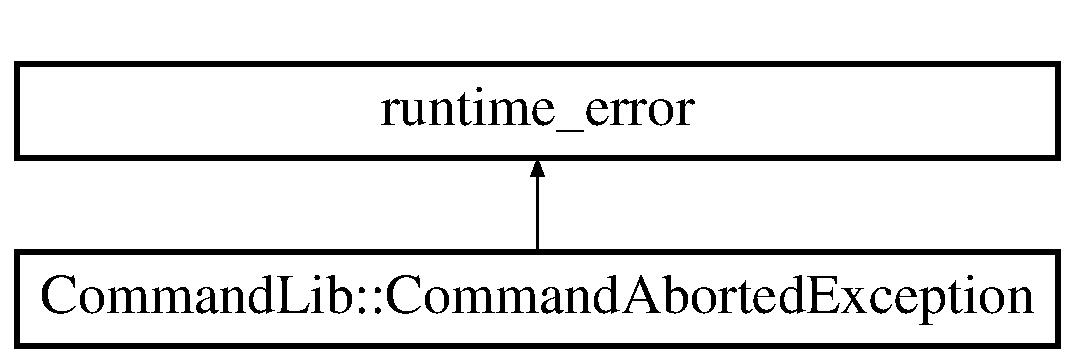
\includegraphics[height=2.000000cm]{class_command_lib_1_1_command_aborted_exception}
\end{center}
\end{figure}
\doxysubsection*{Public Member Functions}
\begin{DoxyCompactItemize}
\item 
\mbox{\hyperlink{class_command_lib_1_1_command_aborted_exception_af5a16bb24375fcba3b2f5c0523d50902}{Command\+Aborted\+Exception}} ()
\begin{DoxyCompactList}\small\item\em Constructs a \mbox{\hyperlink{class_command_lib_1_1_command_aborted_exception}{Command\+Aborted\+Exception}} object \end{DoxyCompactList}\item 
\mbox{\hyperlink{class_command_lib_1_1_command_aborted_exception_ab599bf3faa5161b7c82aa490b0dd6ce3}{Command\+Aborted\+Exception}} (const char $\ast$message)
\begin{DoxyCompactList}\small\item\em Constructs a \mbox{\hyperlink{class_command_lib_1_1_command_aborted_exception}{Command\+Aborted\+Exception}} object \end{DoxyCompactList}\item 
\mbox{\hyperlink{class_command_lib_1_1_command_aborted_exception_a26303ba9a320b9734678fb46575326c4}{Command\+Aborted\+Exception}} (const std\+::string \&message)
\begin{DoxyCompactList}\small\item\em Constructs a \mbox{\hyperlink{class_command_lib_1_1_command_aborted_exception}{Command\+Aborted\+Exception}} object \end{DoxyCompactList}\end{DoxyCompactItemize}


\doxysubsection{Detailed Description}
This is thrown from \mbox{\hyperlink{class_command_lib_1_1_command_a5d33760ccb927d7f6349c02907ab4ff3}{Command.\+Sync\+Execute()}} when a command is aborted. 



\doxysubsection{Constructor \& Destructor Documentation}
\mbox{\Hypertarget{class_command_lib_1_1_command_aborted_exception_af5a16bb24375fcba3b2f5c0523d50902}\label{class_command_lib_1_1_command_aborted_exception_af5a16bb24375fcba3b2f5c0523d50902}} 
\index{CommandLib::CommandAbortedException@{CommandLib::CommandAbortedException}!CommandAbortedException@{CommandAbortedException}}
\index{CommandAbortedException@{CommandAbortedException}!CommandLib::CommandAbortedException@{CommandLib::CommandAbortedException}}
\doxysubsubsection{\texorpdfstring{CommandAbortedException()}{CommandAbortedException()}\hspace{0.1cm}{\footnotesize\ttfamily [1/3]}}
{\footnotesize\ttfamily Command\+Lib\+::\+Command\+Aborted\+Exception\+::\+Command\+Aborted\+Exception (\begin{DoxyParamCaption}{ }\end{DoxyParamCaption})}



Constructs a \mbox{\hyperlink{class_command_lib_1_1_command_aborted_exception}{Command\+Aborted\+Exception}} object 

\mbox{\Hypertarget{class_command_lib_1_1_command_aborted_exception_ab599bf3faa5161b7c82aa490b0dd6ce3}\label{class_command_lib_1_1_command_aborted_exception_ab599bf3faa5161b7c82aa490b0dd6ce3}} 
\index{CommandLib::CommandAbortedException@{CommandLib::CommandAbortedException}!CommandAbortedException@{CommandAbortedException}}
\index{CommandAbortedException@{CommandAbortedException}!CommandLib::CommandAbortedException@{CommandLib::CommandAbortedException}}
\doxysubsubsection{\texorpdfstring{CommandAbortedException()}{CommandAbortedException()}\hspace{0.1cm}{\footnotesize\ttfamily [2/3]}}
{\footnotesize\ttfamily Command\+Lib\+::\+Command\+Aborted\+Exception\+::\+Command\+Aborted\+Exception (\begin{DoxyParamCaption}\item[{const char $\ast$}]{message }\end{DoxyParamCaption})\hspace{0.3cm}{\ttfamily [explicit]}}



Constructs a \mbox{\hyperlink{class_command_lib_1_1_command_aborted_exception}{Command\+Aborted\+Exception}} object 


\begin{DoxyParams}{Parameters}
{\em message} & A description of the reason for abort\\
\hline
\end{DoxyParams}
\mbox{\Hypertarget{class_command_lib_1_1_command_aborted_exception_a26303ba9a320b9734678fb46575326c4}\label{class_command_lib_1_1_command_aborted_exception_a26303ba9a320b9734678fb46575326c4}} 
\index{CommandLib::CommandAbortedException@{CommandLib::CommandAbortedException}!CommandAbortedException@{CommandAbortedException}}
\index{CommandAbortedException@{CommandAbortedException}!CommandLib::CommandAbortedException@{CommandLib::CommandAbortedException}}
\doxysubsubsection{\texorpdfstring{CommandAbortedException()}{CommandAbortedException()}\hspace{0.1cm}{\footnotesize\ttfamily [3/3]}}
{\footnotesize\ttfamily Command\+Lib\+::\+Command\+Aborted\+Exception\+::\+Command\+Aborted\+Exception (\begin{DoxyParamCaption}\item[{const std\+::string \&}]{message }\end{DoxyParamCaption})\hspace{0.3cm}{\ttfamily [explicit]}}



Constructs a \mbox{\hyperlink{class_command_lib_1_1_command_aborted_exception}{Command\+Aborted\+Exception}} object 


\begin{DoxyParams}{Parameters}
{\em message} & A description of the reason for abort\\
\hline
\end{DoxyParams}


The documentation for this class was generated from the following file\+:\begin{DoxyCompactItemize}
\item 
Command\+Lib\+For\+CPP/\+Command\+Lib/include/Command\+Aborted\+Exception.\+h\end{DoxyCompactItemize}

\hypertarget{class_command_lib_1_1_command_dispatcher}{}\doxysection{Command\+Lib\+::Command\+Dispatcher Class Reference}
\label{class_command_lib_1_1_command_dispatcher}\index{CommandLib::CommandDispatcher@{CommandLib::CommandDispatcher}}


Dispatches \mbox{\hyperlink{class_command_lib_1_1_command}{Command}} objects for asynchronous execution.  




{\ttfamily \#include $<$Command\+Dispatcher.\+h$>$}

\doxysubsection*{Public Member Functions}
\begin{DoxyCompactItemize}
\item 
\mbox{\hyperlink{class_command_lib_1_1_command_dispatcher_a9ef89de55c915fbd5f2e61784d67d8a0}{Command\+Dispatcher}} (size\+\_\+t max\+Concurrent)
\begin{DoxyCompactList}\small\item\em Constructs a \mbox{\hyperlink{class_command_lib_1_1_command_dispatcher}{Command\+Dispatcher}} object \end{DoxyCompactList}\item 
void \mbox{\hyperlink{class_command_lib_1_1_command_dispatcher_a2995e97c734165b7d0b3491d606c547b}{Add\+Monitor}} (\mbox{\hyperlink{class_command_lib_1_1_command_monitor}{Command\+Monitor}} $\ast$monitor)
\begin{DoxyCompactList}\small\item\em Adds a listener that will receive callbacks about the status of commands executed by this dispatcher \end{DoxyCompactList}\item 
void \mbox{\hyperlink{class_command_lib_1_1_command_dispatcher_a2a1db45e830c48a4085bb2b86e47c692}{Dispatch}} (\mbox{\hyperlink{class_command_lib_1_1_command_a3b3e4f00144373299df5c6bb1acc319d}{Command\+::\+Ptr}} command)
\begin{DoxyCompactList}\small\item\em If there is room in the pool, asynchronously executes the command immediately. Otherwise, places the command in a queue for processing when room in the pool becomes available. \end{DoxyCompactList}\item 
void \mbox{\hyperlink{class_command_lib_1_1_command_dispatcher_ade1b36f9203de1426d7dff4f83808bec}{Abort}} ()
\begin{DoxyCompactList}\small\item\em Aborts all dispatched commands, and empties the queue of not yet executed commands. \end{DoxyCompactList}\item 
void \mbox{\hyperlink{class_command_lib_1_1_command_dispatcher_ad5f8cae272c637ac628977c1556171c6}{Wait}} ()
\begin{DoxyCompactList}\small\item\em Waits for all dispatched commands to finish execution \end{DoxyCompactList}\item 
void \mbox{\hyperlink{class_command_lib_1_1_command_dispatcher_a324fd9debb368929cbc5357440bd8111}{Abort\+And\+Wait}} ()
\begin{DoxyCompactList}\small\item\em Exact same effect as calling \mbox{\hyperlink{class_command_lib_1_1_command_dispatcher_ade1b36f9203de1426d7dff4f83808bec}{Abort}} followed immediately by a call to \mbox{\hyperlink{class_command_lib_1_1_command_dispatcher_ad5f8cae272c637ac628977c1556171c6}{Wait}}. \end{DoxyCompactList}\end{DoxyCompactItemize}


\doxysubsection{Detailed Description}
Dispatches \mbox{\hyperlink{class_command_lib_1_1_command}{Command}} objects for asynchronous execution. 

This class can be useful when commands are dynamically generated at runtime, and must be dynamically executed upon generation. (for example, asynchronous handling of requests sent over a data stream). 

Upon destruction, this object will wait until all dispatched commands finish execution. For a faster shutdown, you may wish to call \mbox{\hyperlink{class_command_lib_1_1_command_dispatcher_ade1b36f9203de1426d7dff4f83808bec}{Command\+Dispatcher\+::\+Abort()}} before destructing the dispatcher. 

\doxysubsection{Constructor \& Destructor Documentation}
\mbox{\Hypertarget{class_command_lib_1_1_command_dispatcher_a9ef89de55c915fbd5f2e61784d67d8a0}\label{class_command_lib_1_1_command_dispatcher_a9ef89de55c915fbd5f2e61784d67d8a0}} 
\index{CommandLib::CommandDispatcher@{CommandLib::CommandDispatcher}!CommandDispatcher@{CommandDispatcher}}
\index{CommandDispatcher@{CommandDispatcher}!CommandLib::CommandDispatcher@{CommandLib::CommandDispatcher}}
\doxysubsubsection{\texorpdfstring{CommandDispatcher()}{CommandDispatcher()}}
{\footnotesize\ttfamily Command\+Lib\+::\+Command\+Dispatcher\+::\+Command\+Dispatcher (\begin{DoxyParamCaption}\item[{size\+\_\+t}]{max\+Concurrent }\end{DoxyParamCaption})\hspace{0.3cm}{\ttfamily [explicit]}}



Constructs a \mbox{\hyperlink{class_command_lib_1_1_command_dispatcher}{Command\+Dispatcher}} object 


\begin{DoxyParams}{Parameters}
{\em max\+Concurrent} & The maximum number of commands that can be executed concurrently by this dispatcher. If this limit is reached, commands will be queued and only executed when enough prior dispatched commands finish execution. \\
\hline
\end{DoxyParams}


\doxysubsection{Member Function Documentation}
\mbox{\Hypertarget{class_command_lib_1_1_command_dispatcher_ade1b36f9203de1426d7dff4f83808bec}\label{class_command_lib_1_1_command_dispatcher_ade1b36f9203de1426d7dff4f83808bec}} 
\index{CommandLib::CommandDispatcher@{CommandLib::CommandDispatcher}!Abort@{Abort}}
\index{Abort@{Abort}!CommandLib::CommandDispatcher@{CommandLib::CommandDispatcher}}
\doxysubsubsection{\texorpdfstring{Abort()}{Abort()}}
{\footnotesize\ttfamily void Command\+Lib\+::\+Command\+Dispatcher\+::\+Abort (\begin{DoxyParamCaption}{ }\end{DoxyParamCaption})}



Aborts all dispatched commands, and empties the queue of not yet executed commands. 

\mbox{\Hypertarget{class_command_lib_1_1_command_dispatcher_a324fd9debb368929cbc5357440bd8111}\label{class_command_lib_1_1_command_dispatcher_a324fd9debb368929cbc5357440bd8111}} 
\index{CommandLib::CommandDispatcher@{CommandLib::CommandDispatcher}!AbortAndWait@{AbortAndWait}}
\index{AbortAndWait@{AbortAndWait}!CommandLib::CommandDispatcher@{CommandLib::CommandDispatcher}}
\doxysubsubsection{\texorpdfstring{AbortAndWait()}{AbortAndWait()}}
{\footnotesize\ttfamily void Command\+Lib\+::\+Command\+Dispatcher\+::\+Abort\+And\+Wait (\begin{DoxyParamCaption}{ }\end{DoxyParamCaption})}



Exact same effect as calling \mbox{\hyperlink{class_command_lib_1_1_command_dispatcher_ade1b36f9203de1426d7dff4f83808bec}{Abort}} followed immediately by a call to \mbox{\hyperlink{class_command_lib_1_1_command_dispatcher_ad5f8cae272c637ac628977c1556171c6}{Wait}}. 

\mbox{\Hypertarget{class_command_lib_1_1_command_dispatcher_a2995e97c734165b7d0b3491d606c547b}\label{class_command_lib_1_1_command_dispatcher_a2995e97c734165b7d0b3491d606c547b}} 
\index{CommandLib::CommandDispatcher@{CommandLib::CommandDispatcher}!AddMonitor@{AddMonitor}}
\index{AddMonitor@{AddMonitor}!CommandLib::CommandDispatcher@{CommandLib::CommandDispatcher}}
\doxysubsubsection{\texorpdfstring{AddMonitor()}{AddMonitor()}}
{\footnotesize\ttfamily void Command\+Lib\+::\+Command\+Dispatcher\+::\+Add\+Monitor (\begin{DoxyParamCaption}\item[{\mbox{\hyperlink{class_command_lib_1_1_command_monitor}{Command\+Monitor}} $\ast$}]{monitor }\end{DoxyParamCaption})}



Adds a listener that will receive callbacks about the status of commands executed by this dispatcher 

\mbox{\Hypertarget{class_command_lib_1_1_command_dispatcher_a2a1db45e830c48a4085bb2b86e47c692}\label{class_command_lib_1_1_command_dispatcher_a2a1db45e830c48a4085bb2b86e47c692}} 
\index{CommandLib::CommandDispatcher@{CommandLib::CommandDispatcher}!Dispatch@{Dispatch}}
\index{Dispatch@{Dispatch}!CommandLib::CommandDispatcher@{CommandLib::CommandDispatcher}}
\doxysubsubsection{\texorpdfstring{Dispatch()}{Dispatch()}}
{\footnotesize\ttfamily void Command\+Lib\+::\+Command\+Dispatcher\+::\+Dispatch (\begin{DoxyParamCaption}\item[{\mbox{\hyperlink{class_command_lib_1_1_command_a3b3e4f00144373299df5c6bb1acc319d}{Command\+::\+Ptr}}}]{command }\end{DoxyParamCaption})}



If there is room in the pool, asynchronously executes the command immediately. Otherwise, places the command in a queue for processing when room in the pool becomes available. 


\begin{DoxyParams}{Parameters}
{\em command} & The command to execute as soon as there is room in the pool. The command must be top-\/level (that is, it must have no parent). \\
\hline
\end{DoxyParams}
Note that it will cause undefined behavior to dispatch a \mbox{\hyperlink{class_command_lib_1_1_command}{Command}} object that is currently executing, or that has already been dispatched but has not yet executed. 

When the command evenutally finishes execution, the \mbox{\hyperlink{class_command_lib_1_1_command_monitor}{Command\+Monitor}} subscribers will be notified on a different thread. \mbox{\Hypertarget{class_command_lib_1_1_command_dispatcher_ad5f8cae272c637ac628977c1556171c6}\label{class_command_lib_1_1_command_dispatcher_ad5f8cae272c637ac628977c1556171c6}} 
\index{CommandLib::CommandDispatcher@{CommandLib::CommandDispatcher}!Wait@{Wait}}
\index{Wait@{Wait}!CommandLib::CommandDispatcher@{CommandLib::CommandDispatcher}}
\doxysubsubsection{\texorpdfstring{Wait()}{Wait()}}
{\footnotesize\ttfamily void Command\+Lib\+::\+Command\+Dispatcher\+::\+Wait (\begin{DoxyParamCaption}{ }\end{DoxyParamCaption})}



Waits for all dispatched commands to finish execution 



The documentation for this class was generated from the following file\+:\begin{DoxyCompactItemize}
\item 
Command\+Lib\+For\+CPP/\+Command\+Lib/include/Command\+Dispatcher.\+h\end{DoxyCompactItemize}

\hypertarget{class_command_lib_1_1_command_listener}{}\doxysection{Command\+Lib\+::Command\+Listener Class Reference}
\label{class_command_lib_1_1_command_listener}\index{CommandLib::CommandListener@{CommandLib::CommandListener}}


An object implementing this interface is required as a parameter to \mbox{\hyperlink{class_command_lib_1_1_command_a44bad231a0f0a6de3d5405382d95f800}{Command\+::\+Async\+Execute(\+Command\+Listener$\ast$)}}. Exactly one of its methods will eventually be called when a command is executed asynchronously, and it is guaranteed that the call will be on a thread different from the thread Async\+Execute was called from.  




{\ttfamily \#include $<$Command\+Listener.\+h$>$}

\doxysubsection*{Public Member Functions}
\begin{DoxyCompactItemize}
\item 
virtual void \mbox{\hyperlink{class_command_lib_1_1_command_listener_a42f73f4eb4582aa82a0bd1d57151ef73}{Command\+Succeeded}} ()=0
\begin{DoxyCompactList}\small\item\em Called when a \mbox{\hyperlink{class_command_lib_1_1_command}{Command}} launched via \mbox{\hyperlink{class_command_lib_1_1_command_a44bad231a0f0a6de3d5405382d95f800}{Command\+::\+Async\+Execute(\+Command\+Listener$\ast$)}} succeeds. \end{DoxyCompactList}\item 
virtual void \mbox{\hyperlink{class_command_lib_1_1_command_listener_aa389ff6dd3895ce4ecc9447a23e4d9fc}{Command\+Aborted}} ()=0
\begin{DoxyCompactList}\small\item\em Called when a \mbox{\hyperlink{class_command_lib_1_1_command}{Command}} launched via \mbox{\hyperlink{class_command_lib_1_1_command_a44bad231a0f0a6de3d5405382d95f800}{Command\+::\+Async\+Execute(\+Command\+Listener$\ast$)}} was aborted. \end{DoxyCompactList}\item 
virtual void \mbox{\hyperlink{class_command_lib_1_1_command_listener_ae53f9a18ffd79b79754dfdcfb84b138e}{Command\+Failed}} (const std\+::exception \&exc, std\+::exception\+\_\+ptr exc\+Ptr)=0
\end{DoxyCompactItemize}


\doxysubsection{Detailed Description}
An object implementing this interface is required as a parameter to \mbox{\hyperlink{class_command_lib_1_1_command_a44bad231a0f0a6de3d5405382d95f800}{Command\+::\+Async\+Execute(\+Command\+Listener$\ast$)}}. Exactly one of its methods will eventually be called when a command is executed asynchronously, and it is guaranteed that the call will be on a thread different from the thread Async\+Execute was called from. 

The \mbox{\hyperlink{class_command_lib_1_1_command}{Command}} is in the last stage of execution when making these callbacks, so do not re-\/execute the command from within your handler. Also, do not call the executing command\textquotesingle{}s \mbox{\hyperlink{class_command_lib_1_1_command_ac4d49fbf9bbcc543fb57e4b04edf1ddb}{Command\+::\+Wait}} from within your handler, as that will cause deadlock. 

\doxysubsection{Member Function Documentation}
\mbox{\Hypertarget{class_command_lib_1_1_command_listener_aa389ff6dd3895ce4ecc9447a23e4d9fc}\label{class_command_lib_1_1_command_listener_aa389ff6dd3895ce4ecc9447a23e4d9fc}} 
\index{CommandLib::CommandListener@{CommandLib::CommandListener}!CommandAborted@{CommandAborted}}
\index{CommandAborted@{CommandAborted}!CommandLib::CommandListener@{CommandLib::CommandListener}}
\doxysubsubsection{\texorpdfstring{CommandAborted()}{CommandAborted()}}
{\footnotesize\ttfamily virtual void Command\+Lib\+::\+Command\+Listener\+::\+Command\+Aborted (\begin{DoxyParamCaption}{ }\end{DoxyParamCaption})\hspace{0.3cm}{\ttfamily [pure virtual]}}



Called when a \mbox{\hyperlink{class_command_lib_1_1_command}{Command}} launched via \mbox{\hyperlink{class_command_lib_1_1_command_a44bad231a0f0a6de3d5405382d95f800}{Command\+::\+Async\+Execute(\+Command\+Listener$\ast$)}} was aborted. 

The \mbox{\hyperlink{class_command_lib_1_1_command}{Command}} is in the last stage of execution when making this callback, so do not re-\/execute the command from within your handler. Also, do not call the executing command\textquotesingle{}s \mbox{\hyperlink{class_command_lib_1_1_command_ac4d49fbf9bbcc543fb57e4b04edf1ddb}{Command\+::\+Wait}} method from within your handler, as that will cause deadlock. \mbox{\Hypertarget{class_command_lib_1_1_command_listener_ae53f9a18ffd79b79754dfdcfb84b138e}\label{class_command_lib_1_1_command_listener_ae53f9a18ffd79b79754dfdcfb84b138e}} 
\index{CommandLib::CommandListener@{CommandLib::CommandListener}!CommandFailed@{CommandFailed}}
\index{CommandFailed@{CommandFailed}!CommandLib::CommandListener@{CommandLib::CommandListener}}
\doxysubsubsection{\texorpdfstring{CommandFailed()}{CommandFailed()}}
{\footnotesize\ttfamily virtual void Command\+Lib\+::\+Command\+Listener\+::\+Command\+Failed (\begin{DoxyParamCaption}\item[{const std\+::exception \&}]{exc,  }\item[{std\+::exception\+\_\+ptr}]{exc\+Ptr }\end{DoxyParamCaption})\hspace{0.3cm}{\ttfamily [pure virtual]}}





Called when a \mbox{\hyperlink{class_command_lib_1_1_command}{Command}} launched via \mbox{\hyperlink{class_command_lib_1_1_command_a44bad231a0f0a6de3d5405382d95f800}{Command\+::\+Async\+Execute(\+Command\+Listener$\ast$)}} fails.


\begin{DoxyParams}{Parameters}
{\em exc} & The reason for failure\\
\hline
{\em exc\+Ptr} & Allows you to clone the actual error object by calling std\+::rethrow\+\_\+exception. This can be useful if you find yourself \\
\hline
\end{DoxyParams}


The \mbox{\hyperlink{class_command_lib_1_1_command}{Command}} is in the last stage of execution when making this callback, so do not re-\/execute the command from within your handler. Also, do not call the executing command\textquotesingle{}s \mbox{\hyperlink{class_command_lib_1_1_command_ac4d49fbf9bbcc543fb57e4b04edf1ddb}{Command\+::\+Wait}} method from within your handler, as that will cause deadlock. \mbox{\Hypertarget{class_command_lib_1_1_command_listener_a42f73f4eb4582aa82a0bd1d57151ef73}\label{class_command_lib_1_1_command_listener_a42f73f4eb4582aa82a0bd1d57151ef73}} 
\index{CommandLib::CommandListener@{CommandLib::CommandListener}!CommandSucceeded@{CommandSucceeded}}
\index{CommandSucceeded@{CommandSucceeded}!CommandLib::CommandListener@{CommandLib::CommandListener}}
\doxysubsubsection{\texorpdfstring{CommandSucceeded()}{CommandSucceeded()}}
{\footnotesize\ttfamily virtual void Command\+Lib\+::\+Command\+Listener\+::\+Command\+Succeeded (\begin{DoxyParamCaption}{ }\end{DoxyParamCaption})\hspace{0.3cm}{\ttfamily [pure virtual]}}



Called when a \mbox{\hyperlink{class_command_lib_1_1_command}{Command}} launched via \mbox{\hyperlink{class_command_lib_1_1_command_a44bad231a0f0a6de3d5405382d95f800}{Command\+::\+Async\+Execute(\+Command\+Listener$\ast$)}} succeeds. 

The \mbox{\hyperlink{class_command_lib_1_1_command}{Command}} is in the last stage of execution when making this callback, so do not re-\/execute the command from within your handler. Also, do not call the executing command\textquotesingle{}s \mbox{\hyperlink{class_command_lib_1_1_command_ac4d49fbf9bbcc543fb57e4b04edf1ddb}{Command\+::\+Wait}} method from within your handler, as that will cause deadlock. 

The documentation for this class was generated from the following file\+:\begin{DoxyCompactItemize}
\item 
C\+:/\+Users/efiel/source/repos/efieleke/\+Command\+Lib\+For\+CPP/\+Command\+Lib/include/Command\+Listener.\+h\end{DoxyCompactItemize}

\hypertarget{class_command_lib_1_1_command_logger}{}\section{Command\+Lib\+:\+:Command\+Logger Class Reference}
\label{class_command_lib_1_1_command_logger}\index{Command\+Lib\+::\+Command\+Logger@{Command\+Lib\+::\+Command\+Logger}}


Implements \mbox{\hyperlink{class_command_lib_1_1_command_monitor}{Command\+Monitor}} by writing diagnostic information to a log file that can be parsed and dynamically displayed by the Command\+Log\+Viewer application included with the C\# version of this project (found at \href{https://github.com/efieleke/CommandLib.git}{\tt https\+://github.\+com/efieleke/\+Command\+Lib.\+git}).  




{\ttfamily \#include $<$Command\+Logger.\+h$>$}

Inheritance diagram for Command\+Lib\+:\+:Command\+Logger\+:\begin{figure}[H]
\begin{center}
\leavevmode
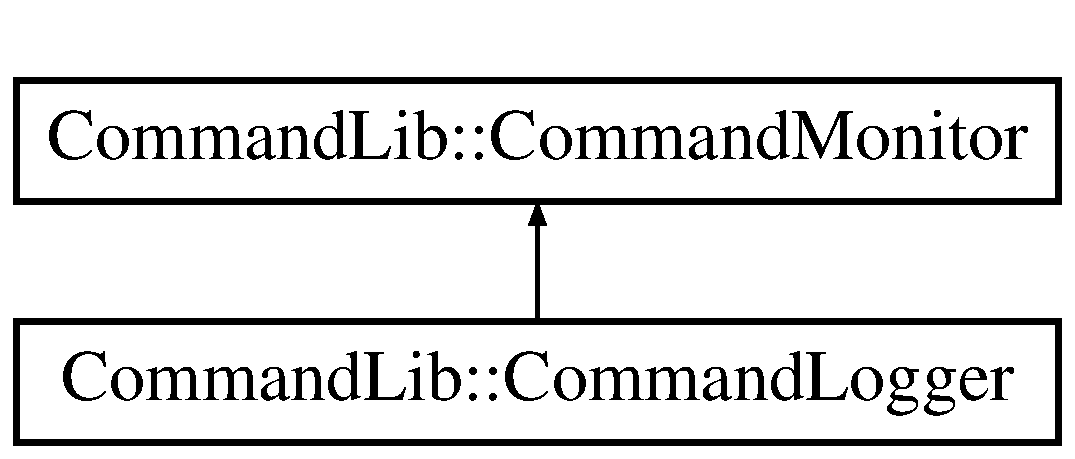
\includegraphics[height=2.000000cm]{class_command_lib_1_1_command_logger}
\end{center}
\end{figure}
\subsection*{Public Member Functions}
\begin{DoxyCompactItemize}
\item 
\mbox{\hyperlink{class_command_lib_1_1_command_logger_ac655a681d1601506900d1a9e879a09e3}{Command\+Logger}} (const std\+::string \&filename)
\begin{DoxyCompactList}\small\item\em Constructor\end{DoxyCompactList}\item 
\mbox{\Hypertarget{class_command_lib_1_1_command_logger_af0094fb705c199e54cf81f3d0accdbf3}\label{class_command_lib_1_1_command_logger_af0094fb705c199e54cf81f3d0accdbf3}} 
virtual void \mbox{\hyperlink{class_command_lib_1_1_command_logger_af0094fb705c199e54cf81f3d0accdbf3}{Command\+Starting}} (const \mbox{\hyperlink{class_command_lib_1_1_command}{Command}} \&command) override
\begin{DoxyCompactList}\small\item\em Invoked when a \mbox{\hyperlink{class_command_lib_1_1_command}{Command}} (including owned commands) starts execution  \end{DoxyCompactList}\item 
\mbox{\Hypertarget{class_command_lib_1_1_command_logger_a445d24aff515f378c9cf3daacd980e22}\label{class_command_lib_1_1_command_logger_a445d24aff515f378c9cf3daacd980e22}} 
virtual void \mbox{\hyperlink{class_command_lib_1_1_command_logger_a445d24aff515f378c9cf3daacd980e22}{Command\+Finished}} (const \mbox{\hyperlink{class_command_lib_1_1_command}{Command}} \&command, const std\+::exception $\ast$exc) override
\begin{DoxyCompactList}\small\item\em Invoked by the framework whenever a \mbox{\hyperlink{class_command_lib_1_1_command}{Command}} (including owned commands) is finishing execution, for whatever reason (success, fail, or abort).  \end{DoxyCompactList}\end{DoxyCompactItemize}


\subsection{Detailed Description}
Implements \mbox{\hyperlink{class_command_lib_1_1_command_monitor}{Command\+Monitor}} by writing diagnostic information to a log file that can be parsed and dynamically displayed by the Command\+Log\+Viewer application included with the C\# version of this project (found at \href{https://github.com/efieleke/CommandLib.git}{\tt https\+://github.\+com/efieleke/\+Command\+Lib.\+git}). 



\subsection{Constructor \& Destructor Documentation}
\mbox{\Hypertarget{class_command_lib_1_1_command_logger_ac655a681d1601506900d1a9e879a09e3}\label{class_command_lib_1_1_command_logger_ac655a681d1601506900d1a9e879a09e3}} 
\index{Command\+Lib\+::\+Command\+Logger@{Command\+Lib\+::\+Command\+Logger}!Command\+Logger@{Command\+Logger}}
\index{Command\+Logger@{Command\+Logger}!Command\+Lib\+::\+Command\+Logger@{Command\+Lib\+::\+Command\+Logger}}
\subsubsection{\texorpdfstring{Command\+Logger()}{CommandLogger()}}
{\footnotesize\ttfamily Command\+Lib\+::\+Command\+Logger\+::\+Command\+Logger (\begin{DoxyParamCaption}\item[{const std\+::string \&}]{filename }\end{DoxyParamCaption})\hspace{0.3cm}{\ttfamily [explicit]}}



Constructor


\begin{DoxyParams}{Parameters}
{\em filename} & Name of the log file. Will be overwritten if it exists.\\
\hline
\end{DoxyParams}


The documentation for this class was generated from the following file\+:\begin{DoxyCompactItemize}
\item 
C\+:/\+Users/efieleke/\+Documents/\+Git\+Hub/\+Command\+Lib\+For\+C\+P\+P/\+Command\+Lib/include/Command\+Logger.\+h\end{DoxyCompactItemize}

\hypertarget{class_command_lib_1_1_command_monitor}{}\doxysection{Command\+Lib\+::Command\+Monitor Class Reference}
\label{class_command_lib_1_1_command_monitor}\index{CommandLib::CommandMonitor@{CommandLib::CommandMonitor}}


This is a callback interface for \mbox{\hyperlink{class_command_lib_1_1_command}{Command}} starting and finishing events. Its intended use is for logging and diagnostics.  




{\ttfamily \#include $<$Command\+Monitor.\+h$>$}

Inheritance diagram for Command\+Lib\+::Command\+Monitor\+:\begin{figure}[H]
\begin{center}
\leavevmode
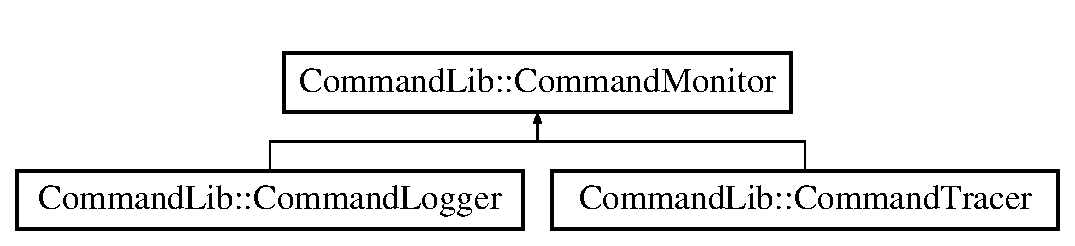
\includegraphics[height=2.000000cm]{class_command_lib_1_1_command_monitor}
\end{center}
\end{figure}
\doxysubsection*{Public Member Functions}
\begin{DoxyCompactItemize}
\item 
virtual void \mbox{\hyperlink{class_command_lib_1_1_command_monitor_a3924a1e128ac5adbf9455b988b56385c}{Command\+Starting}} (const \mbox{\hyperlink{class_command_lib_1_1_command}{Command}} \&command)=0
\begin{DoxyCompactList}\small\item\em Invoked when a \mbox{\hyperlink{class_command_lib_1_1_command}{Command}} (including owned commands) starts execution \end{DoxyCompactList}\item 
virtual void \mbox{\hyperlink{class_command_lib_1_1_command_monitor_a9e140c071319976689d26b5996356cb4}{Command\+Finished}} (const \mbox{\hyperlink{class_command_lib_1_1_command}{Command}} \&command, const std\+::exception $\ast$exc)=0
\begin{DoxyCompactList}\small\item\em Invoked by the framework whenever a \mbox{\hyperlink{class_command_lib_1_1_command}{Command}} (including owned commands) is finishing execution, for whatever reason (success, fail, or abort). \end{DoxyCompactList}\end{DoxyCompactItemize}


\doxysubsection{Detailed Description}
This is a callback interface for \mbox{\hyperlink{class_command_lib_1_1_command}{Command}} starting and finishing events. Its intended use is for logging and diagnostics. 

\mbox{\hyperlink{class_command_lib_1_1_command_tracer}{Command\+Tracer}} and \mbox{\hyperlink{class_command_lib_1_1_command_logger}{Command\+Logger}} are available implementations. You may add a monitor via the static \mbox{\hyperlink{class_command_lib_1_1_command_aa4ceb8d85a720bc5d9bac4be3afd7df5}{Command\+::sm\+\_\+monitors}} member of \mbox{\hyperlink{class_command_lib_1_1_command}{Command}}. Monitors added to that member will be called for every \mbox{\hyperlink{class_command_lib_1_1_command}{Command}} object that executes. To receive callbacks only for commands dispatched via a \mbox{\hyperlink{class_command_lib_1_1_command_dispatcher}{Command\+Dispatcher}}, use \mbox{\hyperlink{class_command_lib_1_1_command_dispatcher_a2995e97c734165b7d0b3491d606c547b}{Command\+Dispatcher\+::\+Add\+Monitor(\+Command\+Monitor$\ast$)}}. 

\doxysubsection{Member Function Documentation}
\mbox{\Hypertarget{class_command_lib_1_1_command_monitor_a9e140c071319976689d26b5996356cb4}\label{class_command_lib_1_1_command_monitor_a9e140c071319976689d26b5996356cb4}} 
\index{CommandLib::CommandMonitor@{CommandLib::CommandMonitor}!CommandFinished@{CommandFinished}}
\index{CommandFinished@{CommandFinished}!CommandLib::CommandMonitor@{CommandLib::CommandMonitor}}
\doxysubsubsection{\texorpdfstring{CommandFinished()}{CommandFinished()}}
{\footnotesize\ttfamily virtual void Command\+Lib\+::\+Command\+Monitor\+::\+Command\+Finished (\begin{DoxyParamCaption}\item[{const \mbox{\hyperlink{class_command_lib_1_1_command}{Command}} \&}]{command,  }\item[{const std\+::exception $\ast$}]{exc }\end{DoxyParamCaption})\hspace{0.3cm}{\ttfamily [pure virtual]}}



Invoked by the framework whenever a \mbox{\hyperlink{class_command_lib_1_1_command}{Command}} (including owned commands) is finishing execution, for whatever reason (success, fail, or abort). 


\begin{DoxyParams}{Parameters}
{\em command} & The command that is finishing execution. \\
\hline
{\em exc} & Will be null if the command succeeded. Otherwise will be a \mbox{\hyperlink{class_command_lib_1_1_command_aborted_exception}{Command\+Aborted\+Exception}} if the command was aborted, or some other Exception type if the command failed. \\
\hline
\end{DoxyParams}


Implementations of this method must not throw. 

Implemented in \mbox{\hyperlink{class_command_lib_1_1_command_tracer_a8ed510ffcee868c92e388d1e3af304d7}{Command\+Lib\+::\+Command\+Tracer}}, and \mbox{\hyperlink{class_command_lib_1_1_command_logger_a445d24aff515f378c9cf3daacd980e22}{Command\+Lib\+::\+Command\+Logger}}.

\mbox{\Hypertarget{class_command_lib_1_1_command_monitor_a3924a1e128ac5adbf9455b988b56385c}\label{class_command_lib_1_1_command_monitor_a3924a1e128ac5adbf9455b988b56385c}} 
\index{CommandLib::CommandMonitor@{CommandLib::CommandMonitor}!CommandStarting@{CommandStarting}}
\index{CommandStarting@{CommandStarting}!CommandLib::CommandMonitor@{CommandLib::CommandMonitor}}
\doxysubsubsection{\texorpdfstring{CommandStarting()}{CommandStarting()}}
{\footnotesize\ttfamily virtual void Command\+Lib\+::\+Command\+Monitor\+::\+Command\+Starting (\begin{DoxyParamCaption}\item[{const \mbox{\hyperlink{class_command_lib_1_1_command}{Command}} \&}]{command }\end{DoxyParamCaption})\hspace{0.3cm}{\ttfamily [pure virtual]}}



Invoked when a \mbox{\hyperlink{class_command_lib_1_1_command}{Command}} (including owned commands) starts execution 


\begin{DoxyParams}{Parameters}
{\em command} & The command that is starting execution. \\
\hline
\end{DoxyParams}


Implementations of this method must not throw. 

Implemented in \mbox{\hyperlink{class_command_lib_1_1_command_tracer_a8bf102840bfad1186d0a693590afd9f9}{Command\+Lib\+::\+Command\+Tracer}}, and \mbox{\hyperlink{class_command_lib_1_1_command_logger_af0094fb705c199e54cf81f3d0accdbf3}{Command\+Lib\+::\+Command\+Logger}}.



The documentation for this class was generated from the following file\+:\begin{DoxyCompactItemize}
\item 
C\+:/\+Users/efiel/source/repos/efieleke/\+Command\+Lib\+For\+CPP/\+Command\+Lib/include/Command\+Monitor.\+h\end{DoxyCompactItemize}

\hypertarget{class_command_lib_1_1_command_timeout_exception}{}\doxysection{Command\+Lib\+::Command\+Timeout\+Exception Class Reference}
\label{class_command_lib_1_1_command_timeout_exception}\index{CommandLib::CommandTimeoutException@{CommandLib::CommandTimeoutException}}


The type of exception thrown by a \mbox{\hyperlink{class_command_lib_1_1_time_limited_command}{Time\+Limited\+Command}} when times runs out  




{\ttfamily \#include $<$Command\+Timeout\+Exception.\+h$>$}

Inheritance diagram for Command\+Lib\+::Command\+Timeout\+Exception\+:\begin{figure}[H]
\begin{center}
\leavevmode
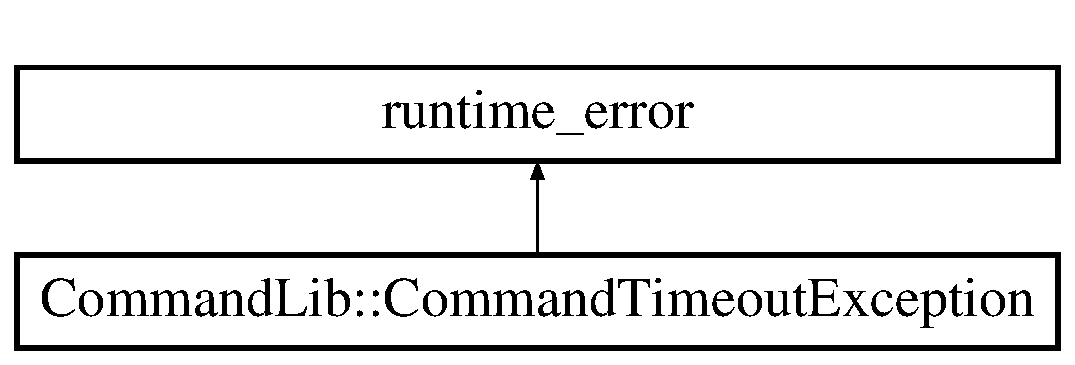
\includegraphics[height=2.000000cm]{class_command_lib_1_1_command_timeout_exception}
\end{center}
\end{figure}
\doxysubsection*{Public Member Functions}
\begin{DoxyCompactItemize}
\item 
\mbox{\hyperlink{class_command_lib_1_1_command_timeout_exception_aad33d69f2a511c9829a3da495aba63e6}{Command\+Timeout\+Exception}} ()
\begin{DoxyCompactList}\small\item\em Constructor \end{DoxyCompactList}\item 
\mbox{\hyperlink{class_command_lib_1_1_command_timeout_exception_a42aa4283bfc20bc9329456f4b75764eb}{Command\+Timeout\+Exception}} (const char $\ast$message)
\begin{DoxyCompactList}\small\item\em Constructor \end{DoxyCompactList}\item 
\mbox{\hyperlink{class_command_lib_1_1_command_timeout_exception_a804d6433419ab58fc046fa2b982f4410}{Command\+Timeout\+Exception}} (const std\+::string \&message)
\begin{DoxyCompactList}\small\item\em Constructor \end{DoxyCompactList}\end{DoxyCompactItemize}


\doxysubsection{Detailed Description}
The type of exception thrown by a \mbox{\hyperlink{class_command_lib_1_1_time_limited_command}{Time\+Limited\+Command}} when times runs out 



\doxysubsection{Constructor \& Destructor Documentation}
\mbox{\Hypertarget{class_command_lib_1_1_command_timeout_exception_aad33d69f2a511c9829a3da495aba63e6}\label{class_command_lib_1_1_command_timeout_exception_aad33d69f2a511c9829a3da495aba63e6}} 
\index{CommandLib::CommandTimeoutException@{CommandLib::CommandTimeoutException}!CommandTimeoutException@{CommandTimeoutException}}
\index{CommandTimeoutException@{CommandTimeoutException}!CommandLib::CommandTimeoutException@{CommandLib::CommandTimeoutException}}
\doxysubsubsection{\texorpdfstring{CommandTimeoutException()}{CommandTimeoutException()}\hspace{0.1cm}{\footnotesize\ttfamily [1/3]}}
{\footnotesize\ttfamily Command\+Lib\+::\+Command\+Timeout\+Exception\+::\+Command\+Timeout\+Exception (\begin{DoxyParamCaption}{ }\end{DoxyParamCaption})}



Constructor 

\mbox{\Hypertarget{class_command_lib_1_1_command_timeout_exception_a42aa4283bfc20bc9329456f4b75764eb}\label{class_command_lib_1_1_command_timeout_exception_a42aa4283bfc20bc9329456f4b75764eb}} 
\index{CommandLib::CommandTimeoutException@{CommandLib::CommandTimeoutException}!CommandTimeoutException@{CommandTimeoutException}}
\index{CommandTimeoutException@{CommandTimeoutException}!CommandLib::CommandTimeoutException@{CommandLib::CommandTimeoutException}}
\doxysubsubsection{\texorpdfstring{CommandTimeoutException()}{CommandTimeoutException()}\hspace{0.1cm}{\footnotesize\ttfamily [2/3]}}
{\footnotesize\ttfamily Command\+Lib\+::\+Command\+Timeout\+Exception\+::\+Command\+Timeout\+Exception (\begin{DoxyParamCaption}\item[{const char $\ast$}]{message }\end{DoxyParamCaption})\hspace{0.3cm}{\ttfamily [explicit]}}



Constructor 


\begin{DoxyParams}{Parameters}
{\em message} & The specific error message, if desired\\
\hline
\end{DoxyParams}
\mbox{\Hypertarget{class_command_lib_1_1_command_timeout_exception_a804d6433419ab58fc046fa2b982f4410}\label{class_command_lib_1_1_command_timeout_exception_a804d6433419ab58fc046fa2b982f4410}} 
\index{CommandLib::CommandTimeoutException@{CommandLib::CommandTimeoutException}!CommandTimeoutException@{CommandTimeoutException}}
\index{CommandTimeoutException@{CommandTimeoutException}!CommandLib::CommandTimeoutException@{CommandLib::CommandTimeoutException}}
\doxysubsubsection{\texorpdfstring{CommandTimeoutException()}{CommandTimeoutException()}\hspace{0.1cm}{\footnotesize\ttfamily [3/3]}}
{\footnotesize\ttfamily Command\+Lib\+::\+Command\+Timeout\+Exception\+::\+Command\+Timeout\+Exception (\begin{DoxyParamCaption}\item[{const std\+::string \&}]{message }\end{DoxyParamCaption})\hspace{0.3cm}{\ttfamily [explicit]}}



Constructor 


\begin{DoxyParams}{Parameters}
{\em message} & The specific error message, if desired\\
\hline
\end{DoxyParams}


The documentation for this class was generated from the following file\+:\begin{DoxyCompactItemize}
\item 
C\+:/\+Users/efiel/source/repos/efieleke/\+Command\+Lib\+For\+CPP/\+Command\+Lib/include/Command\+Timeout\+Exception.\+h\end{DoxyCompactItemize}

\hypertarget{class_command_lib_1_1_command_tracer}{}\doxysection{Command\+Lib\+::Command\+Tracer Class Reference}
\label{class_command_lib_1_1_command_tracer}\index{CommandLib::CommandTracer@{CommandLib::CommandTracer}}


Implements \mbox{\hyperlink{class_command_lib_1_1_command_monitor}{Command\+Monitor}} by writing diagnostic information to an output stream.  




{\ttfamily \#include $<$Command\+Tracer.\+h$>$}

Inheritance diagram for Command\+Lib\+::Command\+Tracer\+:\begin{figure}[H]
\begin{center}
\leavevmode
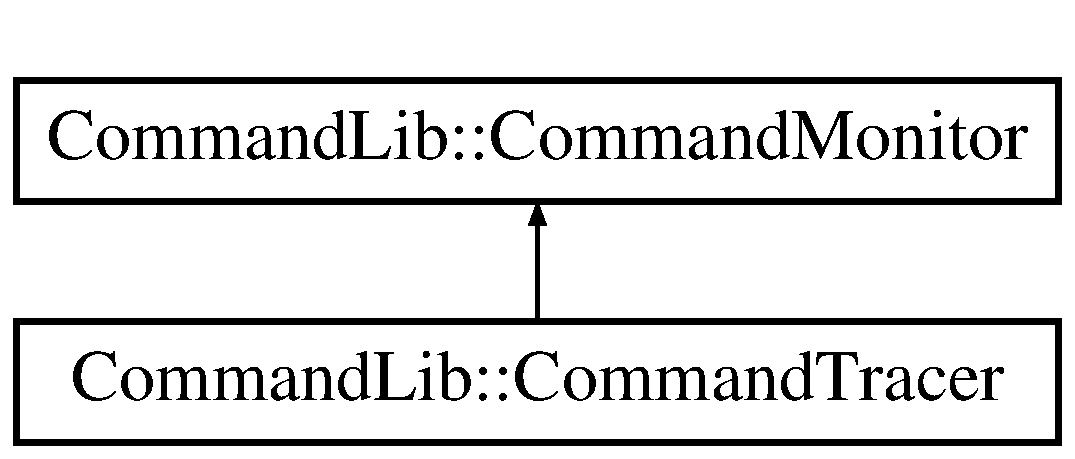
\includegraphics[height=2.000000cm]{class_command_lib_1_1_command_tracer}
\end{center}
\end{figure}
\doxysubsection*{Public Member Functions}
\begin{DoxyCompactItemize}
\item 
\mbox{\hyperlink{class_command_lib_1_1_command_tracer_a415c9eb7f65bbab0356f6beae82a51bf}{Command\+Tracer}} (std\+::ostream \&os)
\begin{DoxyCompactList}\small\item\em Constructor \end{DoxyCompactList}\item 
\mbox{\Hypertarget{class_command_lib_1_1_command_tracer_a8bf102840bfad1186d0a693590afd9f9}\label{class_command_lib_1_1_command_tracer_a8bf102840bfad1186d0a693590afd9f9}} 
virtual void \mbox{\hyperlink{class_command_lib_1_1_command_tracer_a8bf102840bfad1186d0a693590afd9f9}{Command\+Starting}} (const \mbox{\hyperlink{class_command_lib_1_1_command}{Command}} \&command) override
\begin{DoxyCompactList}\small\item\em Invoked when a \mbox{\hyperlink{class_command_lib_1_1_command}{Command}} (including owned commands) starts execution \end{DoxyCompactList}\item 
\mbox{\Hypertarget{class_command_lib_1_1_command_tracer_a8ed510ffcee868c92e388d1e3af304d7}\label{class_command_lib_1_1_command_tracer_a8ed510ffcee868c92e388d1e3af304d7}} 
virtual void \mbox{\hyperlink{class_command_lib_1_1_command_tracer_a8ed510ffcee868c92e388d1e3af304d7}{Command\+Finished}} (const \mbox{\hyperlink{class_command_lib_1_1_command}{Command}} \&command, const std\+::exception $\ast$exc) override
\begin{DoxyCompactList}\small\item\em Invoked by the framework whenever a \mbox{\hyperlink{class_command_lib_1_1_command}{Command}} (including owned commands) is finishing execution, for whatever reason (success, fail, or abort). \end{DoxyCompactList}\end{DoxyCompactItemize}


\doxysubsection{Detailed Description}
Implements \mbox{\hyperlink{class_command_lib_1_1_command_monitor}{Command\+Monitor}} by writing diagnostic information to an output stream. 



\doxysubsection{Constructor \& Destructor Documentation}
\mbox{\Hypertarget{class_command_lib_1_1_command_tracer_a415c9eb7f65bbab0356f6beae82a51bf}\label{class_command_lib_1_1_command_tracer_a415c9eb7f65bbab0356f6beae82a51bf}} 
\index{CommandLib::CommandTracer@{CommandLib::CommandTracer}!CommandTracer@{CommandTracer}}
\index{CommandTracer@{CommandTracer}!CommandLib::CommandTracer@{CommandLib::CommandTracer}}
\doxysubsubsection{\texorpdfstring{CommandTracer()}{CommandTracer()}}
{\footnotesize\ttfamily Command\+Lib\+::\+Command\+Tracer\+::\+Command\+Tracer (\begin{DoxyParamCaption}\item[{std\+::ostream \&}]{os }\end{DoxyParamCaption})\hspace{0.3cm}{\ttfamily [explicit]}}



Constructor 


\begin{DoxyParams}{Parameters}
{\em os} & The stream of which to write output\\
\hline
\end{DoxyParams}


Easiest usage is to just pass std\+::cout as the argument. Windows implementations may wish to define an output stream that wraps Output\+Debug\+Stream 

The documentation for this class was generated from the following file\+:\begin{DoxyCompactItemize}
\item 
C\+:/\+Users/efiel/source/repos/efieleke/\+Command\+Lib\+For\+CPP/\+Command\+Lib/include/Command\+Tracer.\+h\end{DoxyCompactItemize}

\hypertarget{class_command_lib_1_1_event}{}\doxysection{Command\+Lib\+::Event Class Reference}
\label{class_command_lib_1_1_event}\index{CommandLib::Event@{CommandLib::Event}}


This object mimics a Windows manual reset event, and can be added to a \mbox{\hyperlink{class_command_lib_1_1_wait_group}{Wait\+Group}} so that it\textquotesingle{}s possible to wait upon multiple \mbox{\hyperlink{class_command_lib_1_1_event}{Event}} objects.  




{\ttfamily \#include $<$Event.\+h$>$}

Inheritance diagram for Command\+Lib\+::Event\+:\begin{figure}[H]
\begin{center}
\leavevmode
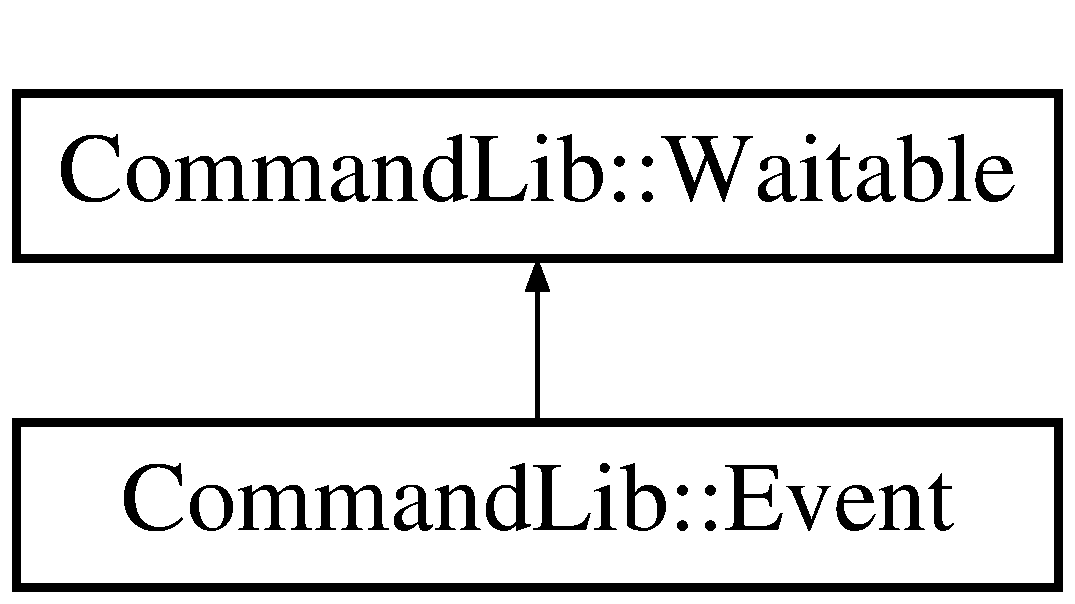
\includegraphics[height=2.000000cm]{class_command_lib_1_1_event}
\end{center}
\end{figure}
\doxysubsection*{Public Types}
\begin{DoxyCompactItemize}
\item 
typedef std\+::shared\+\_\+ptr$<$ \mbox{\hyperlink{class_command_lib_1_1_event}{Event}} $>$ \mbox{\hyperlink{class_command_lib_1_1_event_a3ac4eb982c0456c1216859a61198c073}{Ptr}}
\begin{DoxyCompactList}\small\item\em Shared pointer to an \mbox{\hyperlink{class_command_lib_1_1_event}{Event}} object \end{DoxyCompactList}\end{DoxyCompactItemize}
\doxysubsection*{Public Member Functions}
\begin{DoxyCompactItemize}
\item 
\mbox{\hyperlink{class_command_lib_1_1_event_a165569ddb4788df6b3fad0e52df5e78c}{Event}} ()
\begin{DoxyCompactList}\small\item\em Construct an unsignaled \mbox{\hyperlink{class_command_lib_1_1_event}{Event}} \end{DoxyCompactList}\item 
\mbox{\hyperlink{class_command_lib_1_1_event_a6b00a5faf7e17ea1b5b2984e33309277}{Event}} (bool initially\+Signaled)
\begin{DoxyCompactList}\small\item\em Construct an \mbox{\hyperlink{class_command_lib_1_1_event}{Event}}$>$ \end{DoxyCompactList}\item 
void \mbox{\hyperlink{class_command_lib_1_1_event_a321cb0c97c92012908816b0ced0dcc84}{Set}} ()
\begin{DoxyCompactList}\small\item\em Signal this event \end{DoxyCompactList}\item 
void \mbox{\hyperlink{class_command_lib_1_1_event_a9674a73be80ce75b7438c1d03942bd9e}{Reset}} ()
\begin{DoxyCompactList}\small\item\em Make this event not signaled \end{DoxyCompactList}\item 
\mbox{\Hypertarget{class_command_lib_1_1_event_a943dcf40e6b9fa09df19cd3fa870788e}\label{class_command_lib_1_1_event_a943dcf40e6b9fa09df19cd3fa870788e}} 
virtual bool \mbox{\hyperlink{class_command_lib_1_1_event_a943dcf40e6b9fa09df19cd3fa870788e}{Is\+Signaled}} () const override final
\begin{DoxyCompactList}\small\item\em Indicates whether or not this object is in a signaled state \end{DoxyCompactList}\item 
\mbox{\Hypertarget{class_command_lib_1_1_event_a26986edd42eaa6b85b5a4ddc32af60ae}\label{class_command_lib_1_1_event_a26986edd42eaa6b85b5a4ddc32af60ae}} 
virtual void \mbox{\hyperlink{class_command_lib_1_1_event_a26986edd42eaa6b85b5a4ddc32af60ae}{Wait}} () const override final
\begin{DoxyCompactList}\small\item\em Waits until this object is in a signaled state \end{DoxyCompactList}\item 
\mbox{\Hypertarget{class_command_lib_1_1_event_a395777fd83828fea3d225b2c192d70dd}\label{class_command_lib_1_1_event_a395777fd83828fea3d225b2c192d70dd}} 
virtual bool \mbox{\hyperlink{class_command_lib_1_1_event_a395777fd83828fea3d225b2c192d70dd}{Wait}} (long long ms) const override final
\begin{DoxyCompactList}\small\item\em Waits the given milliseconds until this object is in a signaled state \end{DoxyCompactList}\end{DoxyCompactItemize}
\doxysubsection*{Additional Inherited Members}


\doxysubsection{Detailed Description}
This object mimics a Windows manual reset event, and can be added to a \mbox{\hyperlink{class_command_lib_1_1_wait_group}{Wait\+Group}} so that it\textquotesingle{}s possible to wait upon multiple \mbox{\hyperlink{class_command_lib_1_1_event}{Event}} objects. 



\doxysubsection{Member Typedef Documentation}
\mbox{\Hypertarget{class_command_lib_1_1_event_a3ac4eb982c0456c1216859a61198c073}\label{class_command_lib_1_1_event_a3ac4eb982c0456c1216859a61198c073}} 
\index{CommandLib::Event@{CommandLib::Event}!Ptr@{Ptr}}
\index{Ptr@{Ptr}!CommandLib::Event@{CommandLib::Event}}
\doxysubsubsection{\texorpdfstring{Ptr}{Ptr}}
{\footnotesize\ttfamily typedef std\+::shared\+\_\+ptr$<$\mbox{\hyperlink{class_command_lib_1_1_event}{Event}}$>$ \mbox{\hyperlink{class_command_lib_1_1_event_a3ac4eb982c0456c1216859a61198c073}{Command\+Lib\+::\+Event\+::\+Ptr}}}



Shared pointer to an \mbox{\hyperlink{class_command_lib_1_1_event}{Event}} object 



\doxysubsection{Constructor \& Destructor Documentation}
\mbox{\Hypertarget{class_command_lib_1_1_event_a165569ddb4788df6b3fad0e52df5e78c}\label{class_command_lib_1_1_event_a165569ddb4788df6b3fad0e52df5e78c}} 
\index{CommandLib::Event@{CommandLib::Event}!Event@{Event}}
\index{Event@{Event}!CommandLib::Event@{CommandLib::Event}}
\doxysubsubsection{\texorpdfstring{Event()}{Event()}\hspace{0.1cm}{\footnotesize\ttfamily [1/2]}}
{\footnotesize\ttfamily Command\+Lib\+::\+Event\+::\+Event (\begin{DoxyParamCaption}{ }\end{DoxyParamCaption})}



Construct an unsignaled \mbox{\hyperlink{class_command_lib_1_1_event}{Event}} 

\mbox{\Hypertarget{class_command_lib_1_1_event_a6b00a5faf7e17ea1b5b2984e33309277}\label{class_command_lib_1_1_event_a6b00a5faf7e17ea1b5b2984e33309277}} 
\index{CommandLib::Event@{CommandLib::Event}!Event@{Event}}
\index{Event@{Event}!CommandLib::Event@{CommandLib::Event}}
\doxysubsubsection{\texorpdfstring{Event()}{Event()}\hspace{0.1cm}{\footnotesize\ttfamily [2/2]}}
{\footnotesize\ttfamily Command\+Lib\+::\+Event\+::\+Event (\begin{DoxyParamCaption}\item[{bool}]{initially\+Signaled }\end{DoxyParamCaption})\hspace{0.3cm}{\ttfamily [explicit]}}



Construct an \mbox{\hyperlink{class_command_lib_1_1_event}{Event}}$>$ 


\begin{DoxyParams}{Parameters}
{\em initially\+Signaled} & Whether the event should be initially signaled\\
\hline
\end{DoxyParams}


\doxysubsection{Member Function Documentation}
\mbox{\Hypertarget{class_command_lib_1_1_event_a9674a73be80ce75b7438c1d03942bd9e}\label{class_command_lib_1_1_event_a9674a73be80ce75b7438c1d03942bd9e}} 
\index{CommandLib::Event@{CommandLib::Event}!Reset@{Reset}}
\index{Reset@{Reset}!CommandLib::Event@{CommandLib::Event}}
\doxysubsubsection{\texorpdfstring{Reset()}{Reset()}}
{\footnotesize\ttfamily void Command\+Lib\+::\+Event\+::\+Reset (\begin{DoxyParamCaption}{ }\end{DoxyParamCaption})}



Make this event not signaled 

This object will stay not signaled until \mbox{\hyperlink{class_command_lib_1_1_event_a321cb0c97c92012908816b0ced0dcc84}{Set}} is called. It is safe to call this multiple times in a row. \mbox{\Hypertarget{class_command_lib_1_1_event_a321cb0c97c92012908816b0ced0dcc84}\label{class_command_lib_1_1_event_a321cb0c97c92012908816b0ced0dcc84}} 
\index{CommandLib::Event@{CommandLib::Event}!Set@{Set}}
\index{Set@{Set}!CommandLib::Event@{CommandLib::Event}}
\doxysubsubsection{\texorpdfstring{Set()}{Set()}}
{\footnotesize\ttfamily void Command\+Lib\+::\+Event\+::\+Set (\begin{DoxyParamCaption}{ }\end{DoxyParamCaption})}



Signal this event 

This object will stay signaled until \mbox{\hyperlink{class_command_lib_1_1_event_a9674a73be80ce75b7438c1d03942bd9e}{Reset}} is called. It is safe to call this multiple times in a row. 

The documentation for this class was generated from the following file\+:\begin{DoxyCompactItemize}
\item 
Command\+Lib\+For\+CPP/\+Command\+Lib/include/Event.\+h\end{DoxyCompactItemize}

\hypertarget{class_command_lib_1_1_recurring_command_1_1_execution_time_callback}{}\section{Command\+Lib\+:\+:Recurring\+Command\+:\+:Execution\+Time\+Callback Class Reference}
\label{class_command_lib_1_1_recurring_command_1_1_execution_time_callback}\index{Command\+Lib\+::\+Recurring\+Command\+::\+Execution\+Time\+Callback@{Command\+Lib\+::\+Recurring\+Command\+::\+Execution\+Time\+Callback}}


Defines at what times the underlying command executes  




{\ttfamily \#include $<$Recurring\+Command.\+h$>$}

\subsection*{Public Member Functions}
\begin{DoxyCompactItemize}
\item 
virtual bool \mbox{\hyperlink{class_command_lib_1_1_recurring_command_1_1_execution_time_callback_a5fb9cdbbbcab94a9e4578e0aeaabaa60}{Get\+First\+Execution\+Time}} (std\+::chrono\+::time\+\_\+point$<$ std\+::chrono\+::system\+\_\+clock $>$ $\ast$time)=0
\begin{DoxyCompactList}\small\item\em Called when a $<$see cref\char`\"{}\+Recurring\+Command\char`\"{}/$>$ needs to know the first time to execute its underlying command to run. \end{DoxyCompactList}\item 
virtual bool \mbox{\hyperlink{class_command_lib_1_1_recurring_command_1_1_execution_time_callback_a8ca133b8122f1bf1051bc063a8f67a13}{Get\+Next\+Execution\+Time}} (std\+::chrono\+::time\+\_\+point$<$ std\+::chrono\+::system\+\_\+clock $>$ $\ast$time)=0
\begin{DoxyCompactList}\small\item\em Called when a $<$see cref\char`\"{}\+Recurring\+Command\char`\"{}/$>$ needs to know the next time to execute its underlying command to run. \end{DoxyCompactList}\end{DoxyCompactItemize}


\subsection{Detailed Description}
Defines at what times the underlying command executes 



\subsection{Member Function Documentation}
\mbox{\Hypertarget{class_command_lib_1_1_recurring_command_1_1_execution_time_callback_a5fb9cdbbbcab94a9e4578e0aeaabaa60}\label{class_command_lib_1_1_recurring_command_1_1_execution_time_callback_a5fb9cdbbbcab94a9e4578e0aeaabaa60}} 
\index{Command\+Lib\+::\+Recurring\+Command\+::\+Execution\+Time\+Callback@{Command\+Lib\+::\+Recurring\+Command\+::\+Execution\+Time\+Callback}!Get\+First\+Execution\+Time@{Get\+First\+Execution\+Time}}
\index{Get\+First\+Execution\+Time@{Get\+First\+Execution\+Time}!Command\+Lib\+::\+Recurring\+Command\+::\+Execution\+Time\+Callback@{Command\+Lib\+::\+Recurring\+Command\+::\+Execution\+Time\+Callback}}
\subsubsection{\texorpdfstring{Get\+First\+Execution\+Time()}{GetFirstExecutionTime()}}
{\footnotesize\ttfamily virtual bool Command\+Lib\+::\+Recurring\+Command\+::\+Execution\+Time\+Callback\+::\+Get\+First\+Execution\+Time (\begin{DoxyParamCaption}\item[{std\+::chrono\+::time\+\_\+point$<$ std\+::chrono\+::system\+\_\+clock $>$ $\ast$}]{time }\end{DoxyParamCaption})\hspace{0.3cm}{\ttfamily [pure virtual]}}



Called when a $<$see cref\char`\"{}\+Recurring\+Command\char`\"{}/$>$ needs to know the first time to execute its underlying command to run. 


\begin{DoxyParams}{Parameters}
{\em time} & Implementations should set this to the first time to execute. If a time in the past is specified, the command to run will execute immediately. However, if this method returns false, the value set here will be ignored. \\
\hline
\end{DoxyParams}
\begin{DoxyReturn}{Returns}
Implementations should return true to indicate that the command to run should be executed at the provided time. Returning false causes the \mbox{\hyperlink{class_command_lib_1_1_recurring_command}{Recurring\+Command}} to finish execution. 
\end{DoxyReturn}
\mbox{\Hypertarget{class_command_lib_1_1_recurring_command_1_1_execution_time_callback_a8ca133b8122f1bf1051bc063a8f67a13}\label{class_command_lib_1_1_recurring_command_1_1_execution_time_callback_a8ca133b8122f1bf1051bc063a8f67a13}} 
\index{Command\+Lib\+::\+Recurring\+Command\+::\+Execution\+Time\+Callback@{Command\+Lib\+::\+Recurring\+Command\+::\+Execution\+Time\+Callback}!Get\+Next\+Execution\+Time@{Get\+Next\+Execution\+Time}}
\index{Get\+Next\+Execution\+Time@{Get\+Next\+Execution\+Time}!Command\+Lib\+::\+Recurring\+Command\+::\+Execution\+Time\+Callback@{Command\+Lib\+::\+Recurring\+Command\+::\+Execution\+Time\+Callback}}
\subsubsection{\texorpdfstring{Get\+Next\+Execution\+Time()}{GetNextExecutionTime()}}
{\footnotesize\ttfamily virtual bool Command\+Lib\+::\+Recurring\+Command\+::\+Execution\+Time\+Callback\+::\+Get\+Next\+Execution\+Time (\begin{DoxyParamCaption}\item[{std\+::chrono\+::time\+\_\+point$<$ std\+::chrono\+::system\+\_\+clock $>$ $\ast$}]{time }\end{DoxyParamCaption})\hspace{0.3cm}{\ttfamily [pure virtual]}}



Called when a $<$see cref\char`\"{}\+Recurring\+Command\char`\"{}/$>$ needs to know the next time to execute its underlying command to run. 


\begin{DoxyParams}{Parameters}
{\em time} & This will be initialized to the last time the command to run was set to begin execution. Implementations should set this to the next time to execute. If a time in the past is specified, the command to run will execute immediately. However, if this method returns false, the value set here will be ignored. \\
\hline
\end{DoxyParams}
\begin{DoxyReturn}{Returns}
Implementations should return true to indicate that the command to run should be executed at the provided time. Returning false causes the \mbox{\hyperlink{class_command_lib_1_1_recurring_command}{Recurring\+Command}} to finish execution. 
\end{DoxyReturn}


The documentation for this class was generated from the following file\+:\begin{DoxyCompactItemize}
\item 
C\+:/\+Users/efieleke/\+Documents/\+Git\+Hub/\+Command\+Lib\+For\+C\+P\+P/\+Command\+Lib/include/Recurring\+Command.\+h\end{DoxyCompactItemize}

\hypertarget{class_command_lib_1_1_parallel_commands}{}\section{Command\+Lib\+:\+:Parallel\+Commands Class Reference}
\label{class_command_lib_1_1_parallel_commands}\index{Command\+Lib\+::\+Parallel\+Commands@{Command\+Lib\+::\+Parallel\+Commands}}


Represents a collection of \mbox{\hyperlink{class_command_lib_1_1_command}{Command}} objects that execute in parallel, wrapped in a \mbox{\hyperlink{class_command_lib_1_1_command}{Command}} object 




{\ttfamily \#include $<$Parallel\+Commands.\+h$>$}

Inheritance diagram for Command\+Lib\+:\+:Parallel\+Commands\+:\begin{figure}[H]
\begin{center}
\leavevmode
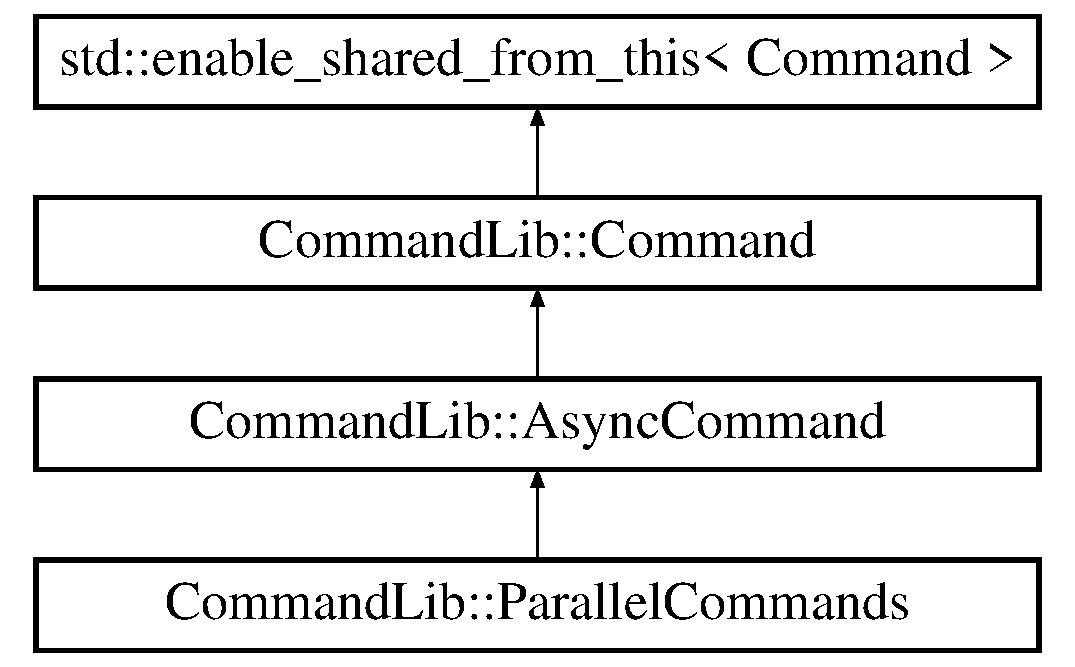
\includegraphics[height=4.000000cm]{class_command_lib_1_1_parallel_commands}
\end{center}
\end{figure}
\subsection*{Public Types}
\begin{DoxyCompactItemize}
\item 
typedef std\+::shared\+\_\+ptr$<$ const \mbox{\hyperlink{class_command_lib_1_1_parallel_commands}{Parallel\+Commands}} $>$ \mbox{\hyperlink{class_command_lib_1_1_parallel_commands_a8ad2164f54391fa1cdffb5d44298580e}{Const\+Ptr}}
\begin{DoxyCompactList}\small\item\em Shared pointer to a non-\/modifyable \mbox{\hyperlink{class_command_lib_1_1_parallel_commands}{Parallel\+Commands}} object\end{DoxyCompactList}\item 
typedef std\+::shared\+\_\+ptr$<$ \mbox{\hyperlink{class_command_lib_1_1_parallel_commands}{Parallel\+Commands}} $>$ \mbox{\hyperlink{class_command_lib_1_1_parallel_commands_affafd160eae15443666daaf2608fd441}{Ptr}}
\begin{DoxyCompactList}\small\item\em Shared pointer to a \mbox{\hyperlink{class_command_lib_1_1_parallel_commands}{Parallel\+Commands}} object\end{DoxyCompactList}\end{DoxyCompactItemize}
\subsection*{Public Member Functions}
\begin{DoxyCompactItemize}
\item 
void \mbox{\hyperlink{class_command_lib_1_1_parallel_commands_a36085841c237794fc8015ed400e552ad}{Add}} (\mbox{\hyperlink{class_command_lib_1_1_command_a3b3e4f00144373299df5c6bb1acc319d}{Command\+::\+Ptr}} command)
\begin{DoxyCompactList}\small\item\em Adds a \mbox{\hyperlink{class_command_lib_1_1_command}{Command}} to the collection to execute.\end{DoxyCompactList}\item 
void \mbox{\hyperlink{class_command_lib_1_1_parallel_commands_aba3f6e3abd06e1483c640eb6d9a82788}{Clear}} ()
\begin{DoxyCompactList}\small\item\em Empties all commands from the collection.\end{DoxyCompactList}\item 
\mbox{\Hypertarget{class_command_lib_1_1_parallel_commands_a5c079ef465fe007bc3b8e893554c5610}\label{class_command_lib_1_1_parallel_commands_a5c079ef465fe007bc3b8e893554c5610}} 
virtual std\+::string \mbox{\hyperlink{class_command_lib_1_1_parallel_commands_a5c079ef465fe007bc3b8e893554c5610}{Extended\+Description}} () const override
\begin{DoxyCompactList}\small\item\em Information about the command (beyond its type and id), if available, for diagnostic purposes.  \end{DoxyCompactList}\item 
\mbox{\Hypertarget{class_command_lib_1_1_parallel_commands_aada3d28f970e82d1d057ac2b499453ac}\label{class_command_lib_1_1_parallel_commands_aada3d28f970e82d1d057ac2b499453ac}} 
virtual std\+::string \mbox{\hyperlink{class_command_lib_1_1_parallel_commands_aada3d28f970e82d1d057ac2b499453ac}{Class\+Name}} () const override
\begin{DoxyCompactList}\small\item\em Gets the name of the runtime instance of this class. Used for logging and diagnostic purposes.  \end{DoxyCompactList}\end{DoxyCompactItemize}
\subsection*{Static Public Member Functions}
\begin{DoxyCompactItemize}
\item 
static \mbox{\hyperlink{class_command_lib_1_1_command_a3b3e4f00144373299df5c6bb1acc319d}{Ptr}} \mbox{\hyperlink{class_command_lib_1_1_parallel_commands_ab75ed6ec91fa1c4652a796a6c0f6868e}{Create}} (bool abort\+Upon\+Failure)
\begin{DoxyCompactList}\small\item\em Creates a \mbox{\hyperlink{class_command_lib_1_1_parallel_commands}{Parallel\+Commands}} object as a top-\/level \mbox{\hyperlink{class_command_lib_1_1_command}{Command}} \end{DoxyCompactList}\end{DoxyCompactItemize}
\subsection*{Protected Member Functions}
\begin{DoxyCompactItemize}
\item 
\mbox{\hyperlink{class_command_lib_1_1_parallel_commands_a795b2df9523b7a154261a52971b29bef}{Parallel\+Commands}} (bool abort\+Upon\+Failure)
\begin{DoxyCompactList}\small\item\em This constructor is not public so as to enforce creation using the \mbox{\hyperlink{class_command_lib_1_1_parallel_commands_ab75ed6ec91fa1c4652a796a6c0f6868e}{Create()}} methods. \end{DoxyCompactList}\end{DoxyCompactItemize}
\subsection*{Additional Inherited Members}


\subsection{Detailed Description}
Represents a collection of \mbox{\hyperlink{class_command_lib_1_1_command}{Command}} objects that execute in parallel, wrapped in a \mbox{\hyperlink{class_command_lib_1_1_command}{Command}} object



\subsection{Member Typedef Documentation}
\mbox{\Hypertarget{class_command_lib_1_1_parallel_commands_a8ad2164f54391fa1cdffb5d44298580e}\label{class_command_lib_1_1_parallel_commands_a8ad2164f54391fa1cdffb5d44298580e}} 
\index{Command\+Lib\+::\+Parallel\+Commands@{Command\+Lib\+::\+Parallel\+Commands}!Const\+Ptr@{Const\+Ptr}}
\index{Const\+Ptr@{Const\+Ptr}!Command\+Lib\+::\+Parallel\+Commands@{Command\+Lib\+::\+Parallel\+Commands}}
\subsubsection{\texorpdfstring{Const\+Ptr}{ConstPtr}}
{\footnotesize\ttfamily typedef std\+::shared\+\_\+ptr$<$const \mbox{\hyperlink{class_command_lib_1_1_parallel_commands}{Parallel\+Commands}}$>$ \mbox{\hyperlink{class_command_lib_1_1_parallel_commands_a8ad2164f54391fa1cdffb5d44298580e}{Command\+Lib\+::\+Parallel\+Commands\+::\+Const\+Ptr}}}



Shared pointer to a non-\/modifyable \mbox{\hyperlink{class_command_lib_1_1_parallel_commands}{Parallel\+Commands}} object

\mbox{\Hypertarget{class_command_lib_1_1_parallel_commands_affafd160eae15443666daaf2608fd441}\label{class_command_lib_1_1_parallel_commands_affafd160eae15443666daaf2608fd441}} 
\index{Command\+Lib\+::\+Parallel\+Commands@{Command\+Lib\+::\+Parallel\+Commands}!Ptr@{Ptr}}
\index{Ptr@{Ptr}!Command\+Lib\+::\+Parallel\+Commands@{Command\+Lib\+::\+Parallel\+Commands}}
\subsubsection{\texorpdfstring{Ptr}{Ptr}}
{\footnotesize\ttfamily typedef std\+::shared\+\_\+ptr$<$\mbox{\hyperlink{class_command_lib_1_1_parallel_commands}{Parallel\+Commands}}$>$ \mbox{\hyperlink{class_command_lib_1_1_parallel_commands_affafd160eae15443666daaf2608fd441}{Command\+Lib\+::\+Parallel\+Commands\+::\+Ptr}}}



Shared pointer to a \mbox{\hyperlink{class_command_lib_1_1_parallel_commands}{Parallel\+Commands}} object



\subsection{Constructor \& Destructor Documentation}
\mbox{\Hypertarget{class_command_lib_1_1_parallel_commands_a795b2df9523b7a154261a52971b29bef}\label{class_command_lib_1_1_parallel_commands_a795b2df9523b7a154261a52971b29bef}} 
\index{Command\+Lib\+::\+Parallel\+Commands@{Command\+Lib\+::\+Parallel\+Commands}!Parallel\+Commands@{Parallel\+Commands}}
\index{Parallel\+Commands@{Parallel\+Commands}!Command\+Lib\+::\+Parallel\+Commands@{Command\+Lib\+::\+Parallel\+Commands}}
\subsubsection{\texorpdfstring{Parallel\+Commands()}{ParallelCommands()}}
{\footnotesize\ttfamily Command\+Lib\+::\+Parallel\+Commands\+::\+Parallel\+Commands (\begin{DoxyParamCaption}\item[{bool}]{abort\+Upon\+Failure }\end{DoxyParamCaption})\hspace{0.3cm}{\ttfamily [explicit]}, {\ttfamily [protected]}}



This constructor is not public so as to enforce creation using the \mbox{\hyperlink{class_command_lib_1_1_parallel_commands_ab75ed6ec91fa1c4652a796a6c0f6868e}{Create()}} methods. 



\subsection{Member Function Documentation}
\mbox{\Hypertarget{class_command_lib_1_1_parallel_commands_a36085841c237794fc8015ed400e552ad}\label{class_command_lib_1_1_parallel_commands_a36085841c237794fc8015ed400e552ad}} 
\index{Command\+Lib\+::\+Parallel\+Commands@{Command\+Lib\+::\+Parallel\+Commands}!Add@{Add}}
\index{Add@{Add}!Command\+Lib\+::\+Parallel\+Commands@{Command\+Lib\+::\+Parallel\+Commands}}
\subsubsection{\texorpdfstring{Add()}{Add()}}
{\footnotesize\ttfamily void Command\+Lib\+::\+Parallel\+Commands\+::\+Add (\begin{DoxyParamCaption}\item[{\mbox{\hyperlink{class_command_lib_1_1_command_a3b3e4f00144373299df5c6bb1acc319d}{Command\+::\+Ptr}}}]{command }\end{DoxyParamCaption})}



Adds a \mbox{\hyperlink{class_command_lib_1_1_command}{Command}} to the collection to execute.


\begin{DoxyParams}{Parameters}
{\em command} & The command to add\\
\hline
\end{DoxyParams}


This object takes ownership of any commands that are added, so the passed command must not already have an owner. 

Behavior is undefined if you add a command while this \mbox{\hyperlink{class_command_lib_1_1_parallel_commands}{Parallel\+Commands}} object is executing

If multiple commands fail, only the first failure reason is reported via \mbox{\hyperlink{class_command_lib_1_1_command_listener}{Command\+Listener}}.\mbox{\Hypertarget{class_command_lib_1_1_parallel_commands_aba3f6e3abd06e1483c640eb6d9a82788}\label{class_command_lib_1_1_parallel_commands_aba3f6e3abd06e1483c640eb6d9a82788}} 
\index{Command\+Lib\+::\+Parallel\+Commands@{Command\+Lib\+::\+Parallel\+Commands}!Clear@{Clear}}
\index{Clear@{Clear}!Command\+Lib\+::\+Parallel\+Commands@{Command\+Lib\+::\+Parallel\+Commands}}
\subsubsection{\texorpdfstring{Clear()}{Clear()}}
{\footnotesize\ttfamily void Command\+Lib\+::\+Parallel\+Commands\+::\+Clear (\begin{DoxyParamCaption}{ }\end{DoxyParamCaption})}



Empties all commands from the collection.

Behavior is undefined if you call this while this command is executing.\mbox{\Hypertarget{class_command_lib_1_1_parallel_commands_ab75ed6ec91fa1c4652a796a6c0f6868e}\label{class_command_lib_1_1_parallel_commands_ab75ed6ec91fa1c4652a796a6c0f6868e}} 
\index{Command\+Lib\+::\+Parallel\+Commands@{Command\+Lib\+::\+Parallel\+Commands}!Create@{Create}}
\index{Create@{Create}!Command\+Lib\+::\+Parallel\+Commands@{Command\+Lib\+::\+Parallel\+Commands}}
\subsubsection{\texorpdfstring{Create()}{Create()}}
{\footnotesize\ttfamily static \mbox{\hyperlink{class_command_lib_1_1_command_a3b3e4f00144373299df5c6bb1acc319d}{Ptr}} Command\+Lib\+::\+Parallel\+Commands\+::\+Create (\begin{DoxyParamCaption}\item[{bool}]{abort\+Upon\+Failure }\end{DoxyParamCaption})\hspace{0.3cm}{\ttfamily [static]}}



Creates a \mbox{\hyperlink{class_command_lib_1_1_parallel_commands}{Parallel\+Commands}} object as a top-\/level \mbox{\hyperlink{class_command_lib_1_1_command}{Command}} 


\begin{DoxyParams}{Parameters}
{\em abort\+Upon\+Failure} & If true, and any \mbox{\hyperlink{class_command_lib_1_1_command}{Command}} within the collection fails, the rest of the executing commands will immediately be aborted \\
\hline
\end{DoxyParams}


The documentation for this class was generated from the following file\+:\begin{DoxyCompactItemize}
\item 
C\+:/\+Users/efieleke/\+Documents/\+Git\+Hub/\+Command\+Lib\+For\+C\+P\+P/\+Command\+Lib/include/Parallel\+Commands.\+h\end{DoxyCompactItemize}

\hypertarget{class_command_lib_1_1_pause_command}{}\doxysection{Command\+Lib\+::Pause\+Command Class Reference}
\label{class_command_lib_1_1_pause_command}\index{CommandLib::PauseCommand@{CommandLib::PauseCommand}}


A \mbox{\hyperlink{class_command_lib_1_1_command}{Command}} that efficiently does nothing for a specified duration.  




{\ttfamily \#include $<$Pause\+Command.\+h$>$}

Inheritance diagram for Command\+Lib\+::Pause\+Command\+:\begin{figure}[H]
\begin{center}
\leavevmode
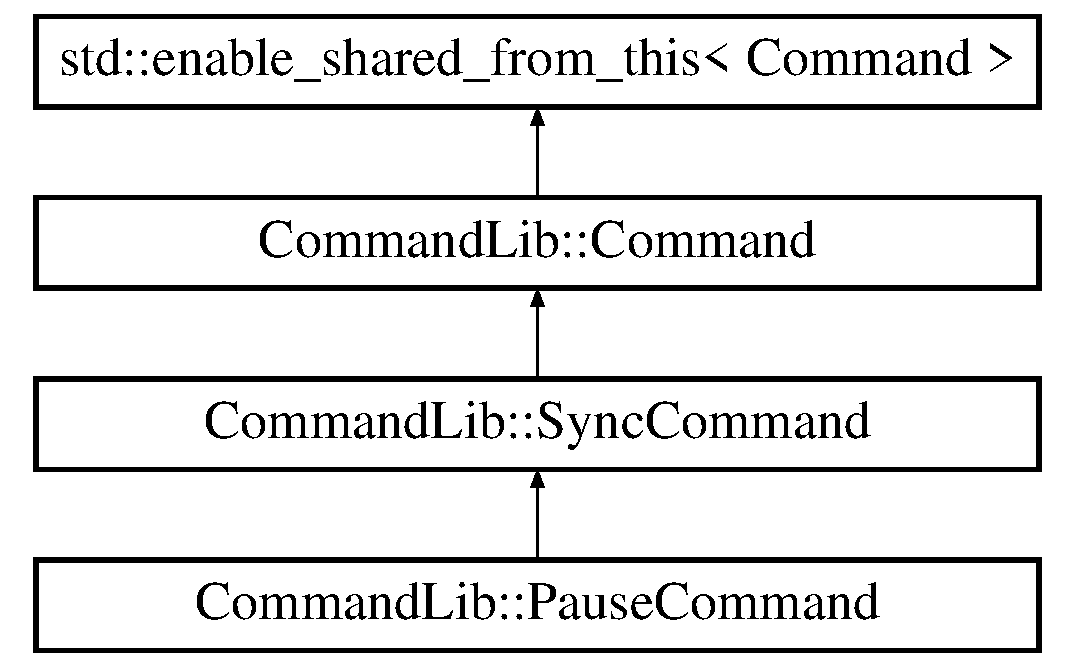
\includegraphics[height=4.000000cm]{class_command_lib_1_1_pause_command}
\end{center}
\end{figure}
\doxysubsection*{Public Types}
\begin{DoxyCompactItemize}
\item 
typedef std\+::shared\+\_\+ptr$<$ const \mbox{\hyperlink{class_command_lib_1_1_pause_command}{Pause\+Command}} $>$ \mbox{\hyperlink{class_command_lib_1_1_pause_command_ad14df8483794045a09d0b08007cbf289}{Const\+Ptr}}
\begin{DoxyCompactList}\small\item\em Shared pointer to a non-\/modifyable \mbox{\hyperlink{class_command_lib_1_1_pause_command}{Pause\+Command}} object \end{DoxyCompactList}\item 
typedef std\+::shared\+\_\+ptr$<$ \mbox{\hyperlink{class_command_lib_1_1_pause_command}{Pause\+Command}} $>$ \mbox{\hyperlink{class_command_lib_1_1_pause_command_ac4c00381b2c560c5d072a0eedaefa92b}{Ptr}}
\begin{DoxyCompactList}\small\item\em Shared pointer to a \mbox{\hyperlink{class_command_lib_1_1_pause_command}{Pause\+Command}} object \end{DoxyCompactList}\end{DoxyCompactItemize}
\doxysubsection*{Public Member Functions}
\begin{DoxyCompactItemize}
\item 
void \mbox{\hyperlink{class_command_lib_1_1_pause_command_a1a02c8ebd44bd32cdc72731d2a16d232}{Cut\+Short}} ()
\begin{DoxyCompactList}\small\item\em If currently executing, finishes the pause now. Does {\itshape not} cause this command to be aborted. \end{DoxyCompactList}\item 
void \mbox{\hyperlink{class_command_lib_1_1_pause_command_abb0980872e2376aece3e184a2decd861}{Reset}} ()
\begin{DoxyCompactList}\small\item\em If currently executing, starts the pause all over again, with the currently set duration value \end{DoxyCompactList}\item 
{\footnotesize template$<$typename Rep , typename Period $>$ }\\std\+::chrono\+::duration$<$ Rep, Period $>$ \mbox{\hyperlink{class_command_lib_1_1_pause_command_aa6bf4dfa9880d58f4995090d0cd6859c}{Get\+Duration}} () const
\begin{DoxyCompactList}\small\item\em Gets the amount of time to pause \end{DoxyCompactList}\item 
long long \mbox{\hyperlink{class_command_lib_1_1_pause_command_a8b92e16e0d088945b64c78437d357cb1}{Get\+Duration\+MS}} () const
\begin{DoxyCompactList}\small\item\em The amount of time to pause in milliseconds \end{DoxyCompactList}\item 
{\footnotesize template$<$typename Rep , typename Period $>$ }\\void \mbox{\hyperlink{class_command_lib_1_1_pause_command_a1ee11b6870b84a56521caa0b8e43c560}{Set\+Duration}} (const std\+::chrono\+::duration$<$ Rep, Period $>$ \&dur)
\begin{DoxyCompactList}\small\item\em Sets the amount of time to pause \end{DoxyCompactList}\item 
void \mbox{\hyperlink{class_command_lib_1_1_pause_command_a87681b8e122468292369874bad63bc8e}{Set\+Duration\+MS}} (long long ms)
\begin{DoxyCompactList}\small\item\em Sets the amount of time to pause in milliseconds \end{DoxyCompactList}\item 
\mbox{\Hypertarget{class_command_lib_1_1_pause_command_a211772cefb139755c74495f190a9a607}\label{class_command_lib_1_1_pause_command_a211772cefb139755c74495f190a9a607}} 
virtual std\+::string \mbox{\hyperlink{class_command_lib_1_1_pause_command_a211772cefb139755c74495f190a9a607}{Extended\+Description}} () const override
\begin{DoxyCompactList}\small\item\em Information about the command (beyond its type and id), if available, for diagnostic purposes. \end{DoxyCompactList}\item 
\mbox{\Hypertarget{class_command_lib_1_1_pause_command_afcdddf1fa8b52a3bfec665b1db736cc5}\label{class_command_lib_1_1_pause_command_afcdddf1fa8b52a3bfec665b1db736cc5}} 
virtual std\+::string \mbox{\hyperlink{class_command_lib_1_1_pause_command_afcdddf1fa8b52a3bfec665b1db736cc5}{Class\+Name}} () const override
\begin{DoxyCompactList}\small\item\em Gets the name of the runtime instance of this class. Used for logging and diagnostic purposes. \end{DoxyCompactList}\end{DoxyCompactItemize}
\doxysubsection*{Static Public Member Functions}
\begin{DoxyCompactItemize}
\item 
{\footnotesize template$<$typename Rep , typename Period $>$ }\\static \mbox{\hyperlink{class_command_lib_1_1_command_a3b3e4f00144373299df5c6bb1acc319d}{Ptr}} \mbox{\hyperlink{class_command_lib_1_1_pause_command_acf08990d56d99bcec76588d786c980e7}{Create}} (const std\+::chrono\+::duration$<$ Rep, Period $>$ \&dur)
\begin{DoxyCompactList}\small\item\em Creates a \mbox{\hyperlink{class_command_lib_1_1_pause_command}{Pause\+Command}} object as a top-\/level \mbox{\hyperlink{class_command_lib_1_1_command}{Command}} \end{DoxyCompactList}\item 
static \mbox{\hyperlink{class_command_lib_1_1_command_a3b3e4f00144373299df5c6bb1acc319d}{Ptr}} \mbox{\hyperlink{class_command_lib_1_1_pause_command_a8c0effc409aae3b87b2126261599f77b}{Create}} (long long ms)
\begin{DoxyCompactList}\small\item\em Creates a \mbox{\hyperlink{class_command_lib_1_1_pause_command}{Pause\+Command}} object as a top-\/level \mbox{\hyperlink{class_command_lib_1_1_command}{Command}} \end{DoxyCompactList}\item 
{\footnotesize template$<$typename Rep , typename Period $>$ }\\static \mbox{\hyperlink{class_command_lib_1_1_command_a3b3e4f00144373299df5c6bb1acc319d}{Ptr}} \mbox{\hyperlink{class_command_lib_1_1_pause_command_a907d1e6292bfbe4af719515534363c40}{Create}} (const std\+::chrono\+::duration$<$ Rep, Period $>$ \&dur, \mbox{\hyperlink{class_command_lib_1_1_waitable_ac74b6b91e48220146eada76a31cf2d9b}{Waitable\+::\+Ptr}} stop\+Event)
\begin{DoxyCompactList}\small\item\em Constructs a \mbox{\hyperlink{class_command_lib_1_1_pause_command}{Pause\+Command}} object as a top-\/level \mbox{\hyperlink{class_command_lib_1_1_command}{Command}} \end{DoxyCompactList}\item 
static \mbox{\hyperlink{class_command_lib_1_1_command_a3b3e4f00144373299df5c6bb1acc319d}{Ptr}} \mbox{\hyperlink{class_command_lib_1_1_pause_command_a76090daf88f99b4e36414a853f3eb447}{Create}} (long long ms, \mbox{\hyperlink{class_command_lib_1_1_waitable_ac74b6b91e48220146eada76a31cf2d9b}{Waitable\+::\+Ptr}} stop\+Event)
\begin{DoxyCompactList}\small\item\em Constructs a \mbox{\hyperlink{class_command_lib_1_1_pause_command}{Pause\+Command}} object as a top-\/level \mbox{\hyperlink{class_command_lib_1_1_command}{Command}} \end{DoxyCompactList}\end{DoxyCompactItemize}
\doxysubsection*{Protected Member Functions}
\begin{DoxyCompactItemize}
\item 
\mbox{\hyperlink{class_command_lib_1_1_pause_command_a777f5a05a5ed78abeafcfbc7e1d27072}{Pause\+Command}} (long long ms, \mbox{\hyperlink{class_command_lib_1_1_waitable_ac74b6b91e48220146eada76a31cf2d9b}{Waitable\+::\+Ptr}} stop\+Event)
\begin{DoxyCompactList}\small\item\em This constructor is not public so as to enforce creation using the \mbox{\hyperlink{class_command_lib_1_1_pause_command_acf08990d56d99bcec76588d786c980e7}{Create()}} methods. \end{DoxyCompactList}\end{DoxyCompactItemize}
\doxysubsection*{Additional Inherited Members}


\doxysubsection{Detailed Description}
A \mbox{\hyperlink{class_command_lib_1_1_command}{Command}} that efficiently does nothing for a specified duration. 



\doxysubsection{Member Typedef Documentation}
\mbox{\Hypertarget{class_command_lib_1_1_pause_command_ad14df8483794045a09d0b08007cbf289}\label{class_command_lib_1_1_pause_command_ad14df8483794045a09d0b08007cbf289}} 
\index{CommandLib::PauseCommand@{CommandLib::PauseCommand}!ConstPtr@{ConstPtr}}
\index{ConstPtr@{ConstPtr}!CommandLib::PauseCommand@{CommandLib::PauseCommand}}
\doxysubsubsection{\texorpdfstring{ConstPtr}{ConstPtr}}
{\footnotesize\ttfamily typedef std\+::shared\+\_\+ptr$<$const \mbox{\hyperlink{class_command_lib_1_1_pause_command}{Pause\+Command}}$>$ \mbox{\hyperlink{class_command_lib_1_1_pause_command_ad14df8483794045a09d0b08007cbf289}{Command\+Lib\+::\+Pause\+Command\+::\+Const\+Ptr}}}



Shared pointer to a non-\/modifyable \mbox{\hyperlink{class_command_lib_1_1_pause_command}{Pause\+Command}} object 

\mbox{\Hypertarget{class_command_lib_1_1_pause_command_ac4c00381b2c560c5d072a0eedaefa92b}\label{class_command_lib_1_1_pause_command_ac4c00381b2c560c5d072a0eedaefa92b}} 
\index{CommandLib::PauseCommand@{CommandLib::PauseCommand}!Ptr@{Ptr}}
\index{Ptr@{Ptr}!CommandLib::PauseCommand@{CommandLib::PauseCommand}}
\doxysubsubsection{\texorpdfstring{Ptr}{Ptr}}
{\footnotesize\ttfamily typedef std\+::shared\+\_\+ptr$<$\mbox{\hyperlink{class_command_lib_1_1_pause_command}{Pause\+Command}}$>$ \mbox{\hyperlink{class_command_lib_1_1_pause_command_ac4c00381b2c560c5d072a0eedaefa92b}{Command\+Lib\+::\+Pause\+Command\+::\+Ptr}}}



Shared pointer to a \mbox{\hyperlink{class_command_lib_1_1_pause_command}{Pause\+Command}} object 



\doxysubsection{Constructor \& Destructor Documentation}
\mbox{\Hypertarget{class_command_lib_1_1_pause_command_a777f5a05a5ed78abeafcfbc7e1d27072}\label{class_command_lib_1_1_pause_command_a777f5a05a5ed78abeafcfbc7e1d27072}} 
\index{CommandLib::PauseCommand@{CommandLib::PauseCommand}!PauseCommand@{PauseCommand}}
\index{PauseCommand@{PauseCommand}!CommandLib::PauseCommand@{CommandLib::PauseCommand}}
\doxysubsubsection{\texorpdfstring{PauseCommand()}{PauseCommand()}}
{\footnotesize\ttfamily Command\+Lib\+::\+Pause\+Command\+::\+Pause\+Command (\begin{DoxyParamCaption}\item[{long long}]{ms,  }\item[{\mbox{\hyperlink{class_command_lib_1_1_waitable_ac74b6b91e48220146eada76a31cf2d9b}{Waitable\+::\+Ptr}}}]{stop\+Event }\end{DoxyParamCaption})\hspace{0.3cm}{\ttfamily [protected]}}



This constructor is not public so as to enforce creation using the \mbox{\hyperlink{class_command_lib_1_1_pause_command_acf08990d56d99bcec76588d786c980e7}{Create()}} methods. 



\doxysubsection{Member Function Documentation}
\mbox{\Hypertarget{class_command_lib_1_1_pause_command_acf08990d56d99bcec76588d786c980e7}\label{class_command_lib_1_1_pause_command_acf08990d56d99bcec76588d786c980e7}} 
\index{CommandLib::PauseCommand@{CommandLib::PauseCommand}!Create@{Create}}
\index{Create@{Create}!CommandLib::PauseCommand@{CommandLib::PauseCommand}}
\doxysubsubsection{\texorpdfstring{Create()}{Create()}\hspace{0.1cm}{\footnotesize\ttfamily [1/4]}}
{\footnotesize\ttfamily template$<$typename Rep , typename Period $>$ \\
static \mbox{\hyperlink{class_command_lib_1_1_command_a3b3e4f00144373299df5c6bb1acc319d}{Ptr}} Command\+Lib\+::\+Pause\+Command\+::\+Create (\begin{DoxyParamCaption}\item[{const std\+::chrono\+::duration$<$ Rep, Period $>$ \&}]{dur }\end{DoxyParamCaption})\hspace{0.3cm}{\ttfamily [inline]}, {\ttfamily [static]}}



Creates a \mbox{\hyperlink{class_command_lib_1_1_pause_command}{Pause\+Command}} object as a top-\/level \mbox{\hyperlink{class_command_lib_1_1_command}{Command}} 


\begin{DoxyParams}{Parameters}
{\em dur} & The amount of time to pause\\
\hline
\end{DoxyParams}


The \mbox{\hyperlink{class_command_lib_1_1_event}{Event}} used in the implemention of this class uses std\+::condition\+\_\+variable\+\_\+any. In my experience, Windows systems will not behave properly if you pass a value that equates to more milliseconds than can fit into the max value of a Windows DWORD (which is under a month long duration). \mbox{\Hypertarget{class_command_lib_1_1_pause_command_a907d1e6292bfbe4af719515534363c40}\label{class_command_lib_1_1_pause_command_a907d1e6292bfbe4af719515534363c40}} 
\index{CommandLib::PauseCommand@{CommandLib::PauseCommand}!Create@{Create}}
\index{Create@{Create}!CommandLib::PauseCommand@{CommandLib::PauseCommand}}
\doxysubsubsection{\texorpdfstring{Create()}{Create()}\hspace{0.1cm}{\footnotesize\ttfamily [2/4]}}
{\footnotesize\ttfamily template$<$typename Rep , typename Period $>$ \\
static \mbox{\hyperlink{class_command_lib_1_1_command_a3b3e4f00144373299df5c6bb1acc319d}{Ptr}} Command\+Lib\+::\+Pause\+Command\+::\+Create (\begin{DoxyParamCaption}\item[{const std\+::chrono\+::duration$<$ Rep, Period $>$ \&}]{dur,  }\item[{\mbox{\hyperlink{class_command_lib_1_1_waitable_ac74b6b91e48220146eada76a31cf2d9b}{Waitable\+::\+Ptr}}}]{stop\+Event }\end{DoxyParamCaption})\hspace{0.3cm}{\ttfamily [inline]}, {\ttfamily [static]}}



Constructs a \mbox{\hyperlink{class_command_lib_1_1_pause_command}{Pause\+Command}} object as a top-\/level \mbox{\hyperlink{class_command_lib_1_1_command}{Command}} 


\begin{DoxyParams}{Parameters}
{\em dur} & The amount of time to pause\\
\hline
{\em stop\+Event} & Optional event to indicate that the \mbox{\hyperlink{class_command_lib_1_1_pause_command}{Pause\+Command}} should stop. Raising this event is equivalent to calling \mbox{\hyperlink{class_command_lib_1_1_pause_command_a1a02c8ebd44bd32cdc72731d2a16d232}{Cut\+Short}} \\
\hline
\end{DoxyParams}


The \mbox{\hyperlink{class_command_lib_1_1_event}{Event}} used in the implemention of this class uses std\+::condition\+\_\+variable\+\_\+any. In my experience, Windows systems will not behave properly if you pass a value that equates to more milliseconds than can fit into the max value of a Windows DWORD (which is under a month long duration). \mbox{\Hypertarget{class_command_lib_1_1_pause_command_a8c0effc409aae3b87b2126261599f77b}\label{class_command_lib_1_1_pause_command_a8c0effc409aae3b87b2126261599f77b}} 
\index{CommandLib::PauseCommand@{CommandLib::PauseCommand}!Create@{Create}}
\index{Create@{Create}!CommandLib::PauseCommand@{CommandLib::PauseCommand}}
\doxysubsubsection{\texorpdfstring{Create()}{Create()}\hspace{0.1cm}{\footnotesize\ttfamily [3/4]}}
{\footnotesize\ttfamily static \mbox{\hyperlink{class_command_lib_1_1_command_a3b3e4f00144373299df5c6bb1acc319d}{Ptr}} Command\+Lib\+::\+Pause\+Command\+::\+Create (\begin{DoxyParamCaption}\item[{long long}]{ms }\end{DoxyParamCaption})\hspace{0.3cm}{\ttfamily [static]}}



Creates a \mbox{\hyperlink{class_command_lib_1_1_pause_command}{Pause\+Command}} object as a top-\/level \mbox{\hyperlink{class_command_lib_1_1_command}{Command}} 


\begin{DoxyParams}{Parameters}
{\em ms} & The number of milliseconds to pause.\\
\hline
\end{DoxyParams}


The \mbox{\hyperlink{class_command_lib_1_1_event}{Event}} used in the implemention of this class uses std\+::condition\+\_\+variable\+\_\+any. In my experience, Windows systems will not behave properly if you pass a value that equates to more milliseconds than can fit into the max value of a Windows DWORD (which is under a month long duration). \mbox{\Hypertarget{class_command_lib_1_1_pause_command_a76090daf88f99b4e36414a853f3eb447}\label{class_command_lib_1_1_pause_command_a76090daf88f99b4e36414a853f3eb447}} 
\index{CommandLib::PauseCommand@{CommandLib::PauseCommand}!Create@{Create}}
\index{Create@{Create}!CommandLib::PauseCommand@{CommandLib::PauseCommand}}
\doxysubsubsection{\texorpdfstring{Create()}{Create()}\hspace{0.1cm}{\footnotesize\ttfamily [4/4]}}
{\footnotesize\ttfamily static \mbox{\hyperlink{class_command_lib_1_1_command_a3b3e4f00144373299df5c6bb1acc319d}{Ptr}} Command\+Lib\+::\+Pause\+Command\+::\+Create (\begin{DoxyParamCaption}\item[{long long}]{ms,  }\item[{\mbox{\hyperlink{class_command_lib_1_1_waitable_ac74b6b91e48220146eada76a31cf2d9b}{Waitable\+::\+Ptr}}}]{stop\+Event }\end{DoxyParamCaption})\hspace{0.3cm}{\ttfamily [static]}}



Constructs a \mbox{\hyperlink{class_command_lib_1_1_pause_command}{Pause\+Command}} object as a top-\/level \mbox{\hyperlink{class_command_lib_1_1_command}{Command}} 


\begin{DoxyParams}{Parameters}
{\em ms} & The number of milliseconds to pause\\
\hline
{\em stop\+Event} & Optional event to indicate that the \mbox{\hyperlink{class_command_lib_1_1_pause_command}{Pause\+Command}} should stop. Raising this event is equivalent to calling \mbox{\hyperlink{class_command_lib_1_1_pause_command_a1a02c8ebd44bd32cdc72731d2a16d232}{Cut\+Short}} \\
\hline
\end{DoxyParams}


The \mbox{\hyperlink{class_command_lib_1_1_event}{Event}} used in the implemention of this class uses std\+::condition\+\_\+variable\+\_\+any. In my experience, Windows systems will not behave properly if you pass a value that equates to more milliseconds than can fit into the max value of a Windows DWORD (which is under a month long duration). \mbox{\Hypertarget{class_command_lib_1_1_pause_command_a1a02c8ebd44bd32cdc72731d2a16d232}\label{class_command_lib_1_1_pause_command_a1a02c8ebd44bd32cdc72731d2a16d232}} 
\index{CommandLib::PauseCommand@{CommandLib::PauseCommand}!CutShort@{CutShort}}
\index{CutShort@{CutShort}!CommandLib::PauseCommand@{CommandLib::PauseCommand}}
\doxysubsubsection{\texorpdfstring{CutShort()}{CutShort()}}
{\footnotesize\ttfamily void Command\+Lib\+::\+Pause\+Command\+::\+Cut\+Short (\begin{DoxyParamCaption}{ }\end{DoxyParamCaption})}



If currently executing, finishes the pause now. Does {\itshape not} cause this command to be aborted. 

\mbox{\Hypertarget{class_command_lib_1_1_pause_command_aa6bf4dfa9880d58f4995090d0cd6859c}\label{class_command_lib_1_1_pause_command_aa6bf4dfa9880d58f4995090d0cd6859c}} 
\index{CommandLib::PauseCommand@{CommandLib::PauseCommand}!GetDuration@{GetDuration}}
\index{GetDuration@{GetDuration}!CommandLib::PauseCommand@{CommandLib::PauseCommand}}
\doxysubsubsection{\texorpdfstring{GetDuration()}{GetDuration()}}
{\footnotesize\ttfamily template$<$typename Rep , typename Period $>$ \\
std\+::chrono\+::duration$<$Rep, Period$>$ Command\+Lib\+::\+Pause\+Command\+::\+Get\+Duration (\begin{DoxyParamCaption}{ }\end{DoxyParamCaption}) const\hspace{0.3cm}{\ttfamily [inline]}}



Gets the amount of time to pause 

\begin{DoxyReturn}{Returns}
The amount of time to pause
\end{DoxyReturn}
\mbox{\Hypertarget{class_command_lib_1_1_pause_command_a8b92e16e0d088945b64c78437d357cb1}\label{class_command_lib_1_1_pause_command_a8b92e16e0d088945b64c78437d357cb1}} 
\index{CommandLib::PauseCommand@{CommandLib::PauseCommand}!GetDurationMS@{GetDurationMS}}
\index{GetDurationMS@{GetDurationMS}!CommandLib::PauseCommand@{CommandLib::PauseCommand}}
\doxysubsubsection{\texorpdfstring{GetDurationMS()}{GetDurationMS()}}
{\footnotesize\ttfamily long long Command\+Lib\+::\+Pause\+Command\+::\+Get\+Duration\+MS (\begin{DoxyParamCaption}{ }\end{DoxyParamCaption}) const}



The amount of time to pause in milliseconds 

\begin{DoxyReturn}{Returns}
The amount of time to pause
\end{DoxyReturn}
\mbox{\Hypertarget{class_command_lib_1_1_pause_command_abb0980872e2376aece3e184a2decd861}\label{class_command_lib_1_1_pause_command_abb0980872e2376aece3e184a2decd861}} 
\index{CommandLib::PauseCommand@{CommandLib::PauseCommand}!Reset@{Reset}}
\index{Reset@{Reset}!CommandLib::PauseCommand@{CommandLib::PauseCommand}}
\doxysubsubsection{\texorpdfstring{Reset()}{Reset()}}
{\footnotesize\ttfamily void Command\+Lib\+::\+Pause\+Command\+::\+Reset (\begin{DoxyParamCaption}{ }\end{DoxyParamCaption})}



If currently executing, starts the pause all over again, with the currently set duration value 

\mbox{\Hypertarget{class_command_lib_1_1_pause_command_a1ee11b6870b84a56521caa0b8e43c560}\label{class_command_lib_1_1_pause_command_a1ee11b6870b84a56521caa0b8e43c560}} 
\index{CommandLib::PauseCommand@{CommandLib::PauseCommand}!SetDuration@{SetDuration}}
\index{SetDuration@{SetDuration}!CommandLib::PauseCommand@{CommandLib::PauseCommand}}
\doxysubsubsection{\texorpdfstring{SetDuration()}{SetDuration()}}
{\footnotesize\ttfamily template$<$typename Rep , typename Period $>$ \\
void Command\+Lib\+::\+Pause\+Command\+::\+Set\+Duration (\begin{DoxyParamCaption}\item[{const std\+::chrono\+::duration$<$ Rep, Period $>$ \&}]{dur }\end{DoxyParamCaption})\hspace{0.3cm}{\ttfamily [inline]}}



Sets the amount of time to pause 


\begin{DoxyParams}{Parameters}
{\em dur} & The amount of time to pause\\
\hline
\end{DoxyParams}


It is safe to change this while the command is executing, but doing so will have no effect until the next time it is executed.\mbox{\Hypertarget{class_command_lib_1_1_pause_command_a87681b8e122468292369874bad63bc8e}\label{class_command_lib_1_1_pause_command_a87681b8e122468292369874bad63bc8e}} 
\index{CommandLib::PauseCommand@{CommandLib::PauseCommand}!SetDurationMS@{SetDurationMS}}
\index{SetDurationMS@{SetDurationMS}!CommandLib::PauseCommand@{CommandLib::PauseCommand}}
\doxysubsubsection{\texorpdfstring{SetDurationMS()}{SetDurationMS()}}
{\footnotesize\ttfamily void Command\+Lib\+::\+Pause\+Command\+::\+Set\+Duration\+MS (\begin{DoxyParamCaption}\item[{long long}]{ms }\end{DoxyParamCaption})}



Sets the amount of time to pause in milliseconds 


\begin{DoxyParams}{Parameters}
{\em ms} & The amount of milliseconds to pause\\
\hline
\end{DoxyParams}


It is safe to change this property while the command is executing, but doing so will have no effect until the next time it is executed.

The documentation for this class was generated from the following file\+:\begin{DoxyCompactItemize}
\item 
C\+:/\+Users/efiel/source/repos/efieleke/\+Command\+Lib\+For\+CPP/\+Command\+Lib/include/Pause\+Command.\+h\end{DoxyCompactItemize}

\hypertarget{class_command_lib_1_1_periodic_command}{}\section{Command\+Lib\+:\+:Periodic\+Command Class Reference}
\label{class_command_lib_1_1_periodic_command}\index{Command\+Lib\+::\+Periodic\+Command@{Command\+Lib\+::\+Periodic\+Command}}


Represents a \mbox{\hyperlink{class_command_lib_1_1_command}{Command}} that repeats periodically at a specified interval 




{\ttfamily \#include $<$Periodic\+Command.\+h$>$}

Inheritance diagram for Command\+Lib\+:\+:Periodic\+Command\+:\begin{figure}[H]
\begin{center}
\leavevmode
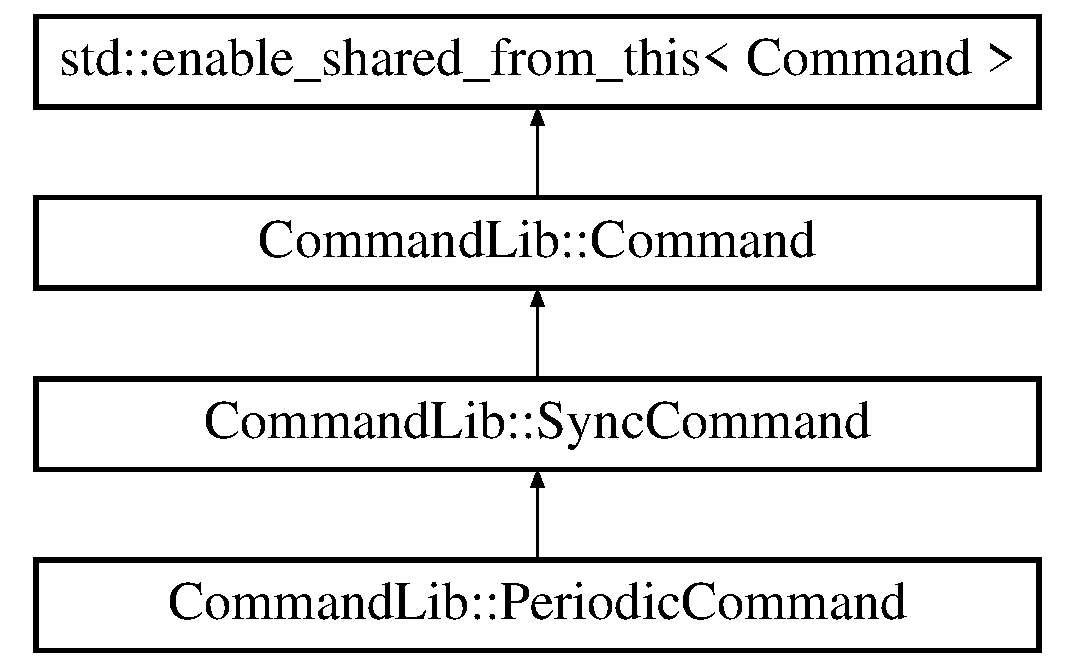
\includegraphics[height=4.000000cm]{class_command_lib_1_1_periodic_command}
\end{center}
\end{figure}
\subsection*{Public Types}
\begin{DoxyCompactItemize}
\item 
enum \mbox{\hyperlink{class_command_lib_1_1_periodic_command_ac32ef93cf679cd652da30a0ad373d31e}{Interval\+Type}} \{ \mbox{\hyperlink{class_command_lib_1_1_periodic_command_ac32ef93cf679cd652da30a0ad373d31ea9df9cbfe0251b1b5670ee8ce058bd287}{Interval\+Type\+::\+Pause\+Before}}, 
\mbox{\hyperlink{class_command_lib_1_1_periodic_command_ac32ef93cf679cd652da30a0ad373d31ea4ccaa10bfe2d79ac758dfa35d4ca588f}{Interval\+Type\+::\+Pause\+After}}
 \}
\begin{DoxyCompactList}\small\item\em Defines how the interval between command executions is performed within a \mbox{\hyperlink{class_command_lib_1_1_periodic_command}{Periodic\+Command}} \end{DoxyCompactList}\item 
typedef std\+::shared\+\_\+ptr$<$ const \mbox{\hyperlink{class_command_lib_1_1_periodic_command}{Periodic\+Command}} $>$ \mbox{\hyperlink{class_command_lib_1_1_periodic_command_ad004e7ccaad4b0413f341dac73d050fc}{Const\+Ptr}}
\begin{DoxyCompactList}\small\item\em Shared pointer to a non-\/modifyable \mbox{\hyperlink{class_command_lib_1_1_periodic_command}{Periodic\+Command}} object\end{DoxyCompactList}\item 
typedef std\+::shared\+\_\+ptr$<$ \mbox{\hyperlink{class_command_lib_1_1_periodic_command}{Periodic\+Command}} $>$ \mbox{\hyperlink{class_command_lib_1_1_periodic_command_a4aa1af2412d7688c7b9a5d76b240b38a}{Ptr}}
\begin{DoxyCompactList}\small\item\em Shared pointer to a \mbox{\hyperlink{class_command_lib_1_1_periodic_command}{Periodic\+Command}} object\end{DoxyCompactList}\end{DoxyCompactItemize}
\subsection*{Public Member Functions}
\begin{DoxyCompactItemize}
\item 
{\footnotesize template$<$typename Unit $>$ }\\Unit \mbox{\hyperlink{class_command_lib_1_1_periodic_command_a4be16b8f26b54d9ca41f01f723eb7faf}{Get\+Interval}} () const
\begin{DoxyCompactList}\small\item\em Gets the interval of time between command executions. \end{DoxyCompactList}\item 
{\footnotesize template$<$typename Rep , typename Period $>$ }\\void \mbox{\hyperlink{class_command_lib_1_1_periodic_command_af344626ecaa9e0ecb85fd2f98100eba9}{Set\+Interval}} (const std\+::chrono\+::duration$<$ Rep, Period $>$ \&interval)
\begin{DoxyCompactList}\small\item\em Sets the interval of time between command executions. \end{DoxyCompactList}\item 
long long \mbox{\hyperlink{class_command_lib_1_1_periodic_command_abef034455e746be6367651cc05702344}{Get\+Interval\+MS}} () const
\begin{DoxyCompactList}\small\item\em Gets the interval of time between command executions in milliseconds. \end{DoxyCompactList}\item 
void \mbox{\hyperlink{class_command_lib_1_1_periodic_command_ae4f9588a25154969bfb9dbf10cf5e367}{Set\+Interval\+MS}} (long long interval)
\begin{DoxyCompactList}\small\item\em Sets the number of milliseconds between command executions. \end{DoxyCompactList}\item 
void \mbox{\hyperlink{class_command_lib_1_1_periodic_command_a59a83d1c32419d61d326040d7aa040ef}{Stop}} ()
\begin{DoxyCompactList}\small\item\em Causes the command to stop repeating. This will not cause the command to be aborted. If the command to run is currently executing when this is called, it will be allowed to finish. \end{DoxyCompactList}\item 
void \mbox{\hyperlink{class_command_lib_1_1_periodic_command_a537aa24d843d7ca7a4fe1d9a9e5f1d24}{Skip\+Current\+Wait}} ()
\begin{DoxyCompactList}\small\item\em If currently in the interval between command executions, skips the wait and executes the command right away. This only skips the current wait. It will not skip subsequent waits. \end{DoxyCompactList}\item 
void \mbox{\hyperlink{class_command_lib_1_1_periodic_command_ad07aa39b59712f784b16419fe055783c}{Reset}} ()
\begin{DoxyCompactList}\small\item\em Rewinds the current pause to its full duration. \end{DoxyCompactList}\item 
virtual std\+::string \mbox{\hyperlink{class_command_lib_1_1_periodic_command_a330571debdbd7f7b306dd7f2718e84e5}{Extended\+Description}} () const override
\begin{DoxyCompactList}\small\item\em Returns diagnostic information about this object\textquotesingle{}s state \end{DoxyCompactList}\item 
\mbox{\Hypertarget{class_command_lib_1_1_periodic_command_a77c34a0f31ae4e7f0c642a356bd5d6ef}\label{class_command_lib_1_1_periodic_command_a77c34a0f31ae4e7f0c642a356bd5d6ef}} 
virtual std\+::string \mbox{\hyperlink{class_command_lib_1_1_periodic_command_a77c34a0f31ae4e7f0c642a356bd5d6ef}{Class\+Name}} () const override
\begin{DoxyCompactList}\small\item\em Gets the name of the runtime instance of this class. Used for logging and diagnostic purposes.  \end{DoxyCompactList}\end{DoxyCompactItemize}
\subsection*{Static Public Member Functions}
\begin{DoxyCompactItemize}
\item 
{\footnotesize template$<$typename Rep , typename Period $>$ }\\static \mbox{\hyperlink{class_command_lib_1_1_command_a3b3e4f00144373299df5c6bb1acc319d}{Ptr}} \mbox{\hyperlink{class_command_lib_1_1_periodic_command_aa553fa62e0e5774b39c1105caf3dd087}{Create}} (\mbox{\hyperlink{class_command_lib_1_1_command_a3b3e4f00144373299df5c6bb1acc319d}{Command\+::\+Ptr}} command, size\+\_\+t repeat\+Count, std\+::chrono\+::duration$<$ Rep, Period $>$ interval, \mbox{\hyperlink{class_command_lib_1_1_periodic_command_ac32ef93cf679cd652da30a0ad373d31e}{Interval\+Type}} interval\+Type, bool interval\+Is\+Inclusive)
\begin{DoxyCompactList}\small\item\em Creates a \mbox{\hyperlink{class_command_lib_1_1_periodic_command}{Periodic\+Command}} \end{DoxyCompactList}\item 
static \mbox{\hyperlink{class_command_lib_1_1_command_a3b3e4f00144373299df5c6bb1acc319d}{Ptr}} \mbox{\hyperlink{class_command_lib_1_1_periodic_command_aa6ae89b0c0a0a61388748856074596b8}{Create}} (\mbox{\hyperlink{class_command_lib_1_1_command_a3b3e4f00144373299df5c6bb1acc319d}{Command\+::\+Ptr}} command, size\+\_\+t repeat\+Count, long long interval\+MS, \mbox{\hyperlink{class_command_lib_1_1_periodic_command_ac32ef93cf679cd652da30a0ad373d31e}{Interval\+Type}} interval\+Type, bool interval\+Is\+Inclusive)
\begin{DoxyCompactList}\small\item\em Creates a \mbox{\hyperlink{class_command_lib_1_1_periodic_command}{Periodic\+Command}} \end{DoxyCompactList}\item 
{\footnotesize template$<$typename Rep , typename Period $>$ }\\static \mbox{\hyperlink{class_command_lib_1_1_command_a3b3e4f00144373299df5c6bb1acc319d}{Ptr}} \mbox{\hyperlink{class_command_lib_1_1_periodic_command_a22783c7b42c443ebe6a6392d380efe51}{Create}} (\mbox{\hyperlink{class_command_lib_1_1_command_a3b3e4f00144373299df5c6bb1acc319d}{Command\+::\+Ptr}} command, size\+\_\+t repeat\+Count, std\+::chrono\+::duration$<$ Rep, Period $>$ interval, \mbox{\hyperlink{class_command_lib_1_1_periodic_command_ac32ef93cf679cd652da30a0ad373d31e}{Interval\+Type}} interval\+Type, bool interval\+Is\+Inclusive, \mbox{\hyperlink{class_command_lib_1_1_waitable_ac74b6b91e48220146eada76a31cf2d9b}{Waitable\+::\+Ptr}} stop\+Event)
\begin{DoxyCompactList}\small\item\em Creates a \mbox{\hyperlink{class_command_lib_1_1_periodic_command}{Periodic\+Command}} \end{DoxyCompactList}\item 
static \mbox{\hyperlink{class_command_lib_1_1_command_a3b3e4f00144373299df5c6bb1acc319d}{Ptr}} \mbox{\hyperlink{class_command_lib_1_1_periodic_command_aeaa8112e6cab67aa63eb906bea96e5d2}{Create}} (\mbox{\hyperlink{class_command_lib_1_1_command_a3b3e4f00144373299df5c6bb1acc319d}{Command\+::\+Ptr}} command, size\+\_\+t repeat\+Count, long long interval\+MS, \mbox{\hyperlink{class_command_lib_1_1_periodic_command_ac32ef93cf679cd652da30a0ad373d31e}{Interval\+Type}} interval\+Type, bool interval\+Is\+Inclusive, \mbox{\hyperlink{class_command_lib_1_1_waitable_ac74b6b91e48220146eada76a31cf2d9b}{Waitable\+::\+Ptr}} stop\+Event)
\begin{DoxyCompactList}\small\item\em Creates a \mbox{\hyperlink{class_command_lib_1_1_periodic_command}{Periodic\+Command}} \end{DoxyCompactList}\end{DoxyCompactItemize}
\subsection*{Public Attributes}
\begin{DoxyCompactItemize}
\item 
std\+::atomic\+\_\+uint \mbox{\hyperlink{class_command_lib_1_1_periodic_command_ab6e63dc1cc0fa2dc39eded7ca5f1fd94}{m\+\_\+repeat\+Count}}
\begin{DoxyCompactList}\small\item\em The total number of times the command to run will execute. If the command to run is currently executing when this is changed, it will be allowed to finish, even if the repeat count is set to a number lower than the number of times already executed. \end{DoxyCompactList}\end{DoxyCompactItemize}
\subsection*{Protected Member Functions}
\begin{DoxyCompactItemize}
\item 
\mbox{\hyperlink{class_command_lib_1_1_periodic_command_ae01a26a099f4ffd1006e9d8451568964}{Periodic\+Command}} (\mbox{\hyperlink{class_command_lib_1_1_command_a3b3e4f00144373299df5c6bb1acc319d}{Command\+::\+Ptr}} command, size\+\_\+t repeat\+Count, long long interval\+MS, \mbox{\hyperlink{class_command_lib_1_1_periodic_command_ac32ef93cf679cd652da30a0ad373d31e}{Interval\+Type}} interval\+Type, bool interval\+Is\+Inclusive, \mbox{\hyperlink{class_command_lib_1_1_waitable_ac74b6b91e48220146eada76a31cf2d9b}{Waitable\+::\+Ptr}} stop\+Event)
\begin{DoxyCompactList}\small\item\em This constructor is not public so as to enforce creation using the \mbox{\hyperlink{class_command_lib_1_1_periodic_command_aa553fa62e0e5774b39c1105caf3dd087}{Create()}} methods. \end{DoxyCompactList}\end{DoxyCompactItemize}
\subsection*{Additional Inherited Members}


\subsection{Detailed Description}
Represents a \mbox{\hyperlink{class_command_lib_1_1_command}{Command}} that repeats periodically at a specified interval

If more dynamic control is needed around the period of time between executions, use \mbox{\hyperlink{class_command_lib_1_1_recurring_command}{Recurring\+Command}} instead. 

\subsection{Member Typedef Documentation}
\mbox{\Hypertarget{class_command_lib_1_1_periodic_command_ad004e7ccaad4b0413f341dac73d050fc}\label{class_command_lib_1_1_periodic_command_ad004e7ccaad4b0413f341dac73d050fc}} 
\index{Command\+Lib\+::\+Periodic\+Command@{Command\+Lib\+::\+Periodic\+Command}!Const\+Ptr@{Const\+Ptr}}
\index{Const\+Ptr@{Const\+Ptr}!Command\+Lib\+::\+Periodic\+Command@{Command\+Lib\+::\+Periodic\+Command}}
\subsubsection{\texorpdfstring{Const\+Ptr}{ConstPtr}}
{\footnotesize\ttfamily typedef std\+::shared\+\_\+ptr$<$const \mbox{\hyperlink{class_command_lib_1_1_periodic_command}{Periodic\+Command}}$>$ \mbox{\hyperlink{class_command_lib_1_1_periodic_command_ad004e7ccaad4b0413f341dac73d050fc}{Command\+Lib\+::\+Periodic\+Command\+::\+Const\+Ptr}}}



Shared pointer to a non-\/modifyable \mbox{\hyperlink{class_command_lib_1_1_periodic_command}{Periodic\+Command}} object

\mbox{\Hypertarget{class_command_lib_1_1_periodic_command_a4aa1af2412d7688c7b9a5d76b240b38a}\label{class_command_lib_1_1_periodic_command_a4aa1af2412d7688c7b9a5d76b240b38a}} 
\index{Command\+Lib\+::\+Periodic\+Command@{Command\+Lib\+::\+Periodic\+Command}!Ptr@{Ptr}}
\index{Ptr@{Ptr}!Command\+Lib\+::\+Periodic\+Command@{Command\+Lib\+::\+Periodic\+Command}}
\subsubsection{\texorpdfstring{Ptr}{Ptr}}
{\footnotesize\ttfamily typedef std\+::shared\+\_\+ptr$<$\mbox{\hyperlink{class_command_lib_1_1_periodic_command}{Periodic\+Command}}$>$ \mbox{\hyperlink{class_command_lib_1_1_periodic_command_a4aa1af2412d7688c7b9a5d76b240b38a}{Command\+Lib\+::\+Periodic\+Command\+::\+Ptr}}}



Shared pointer to a \mbox{\hyperlink{class_command_lib_1_1_periodic_command}{Periodic\+Command}} object



\subsection{Member Enumeration Documentation}
\mbox{\Hypertarget{class_command_lib_1_1_periodic_command_ac32ef93cf679cd652da30a0ad373d31e}\label{class_command_lib_1_1_periodic_command_ac32ef93cf679cd652da30a0ad373d31e}} 
\index{Command\+Lib\+::\+Periodic\+Command@{Command\+Lib\+::\+Periodic\+Command}!Interval\+Type@{Interval\+Type}}
\index{Interval\+Type@{Interval\+Type}!Command\+Lib\+::\+Periodic\+Command@{Command\+Lib\+::\+Periodic\+Command}}
\subsubsection{\texorpdfstring{Interval\+Type}{IntervalType}}
{\footnotesize\ttfamily enum \mbox{\hyperlink{class_command_lib_1_1_periodic_command_ac32ef93cf679cd652da30a0ad373d31e}{Command\+Lib\+::\+Periodic\+Command\+::\+Interval\+Type}}\hspace{0.3cm}{\ttfamily [strong]}}



Defines how the interval between command executions is performed within a \mbox{\hyperlink{class_command_lib_1_1_periodic_command}{Periodic\+Command}} 

\begin{DoxyEnumFields}{Enumerator}
\raisebox{\heightof{T}}[0pt][0pt]{\index{Pause\+Before@{Pause\+Before}!Command\+Lib\+::\+Periodic\+Command@{Command\+Lib\+::\+Periodic\+Command}}\index{Command\+Lib\+::\+Periodic\+Command@{Command\+Lib\+::\+Periodic\+Command}!Pause\+Before@{Pause\+Before}}}\mbox{\Hypertarget{class_command_lib_1_1_periodic_command_ac32ef93cf679cd652da30a0ad373d31ea9df9cbfe0251b1b5670ee8ce058bd287}\label{class_command_lib_1_1_periodic_command_ac32ef93cf679cd652da30a0ad373d31ea9df9cbfe0251b1b5670ee8ce058bd287}} 
Pause\+Before&Pause first, then run the command, and repeat as many times as specified \\
\hline

\raisebox{\heightof{T}}[0pt][0pt]{\index{Pause\+After@{Pause\+After}!Command\+Lib\+::\+Periodic\+Command@{Command\+Lib\+::\+Periodic\+Command}}\index{Command\+Lib\+::\+Periodic\+Command@{Command\+Lib\+::\+Periodic\+Command}!Pause\+After@{Pause\+After}}}\mbox{\Hypertarget{class_command_lib_1_1_periodic_command_ac32ef93cf679cd652da30a0ad373d31ea4ccaa10bfe2d79ac758dfa35d4ca588f}\label{class_command_lib_1_1_periodic_command_ac32ef93cf679cd652da30a0ad373d31ea4ccaa10bfe2d79ac758dfa35d4ca588f}} 
Pause\+After&Run the command first, then pause, and repeat as many times as specified. There is no pause after the last execution of the command. \\
\hline

\end{DoxyEnumFields}


\subsection{Constructor \& Destructor Documentation}
\mbox{\Hypertarget{class_command_lib_1_1_periodic_command_ae01a26a099f4ffd1006e9d8451568964}\label{class_command_lib_1_1_periodic_command_ae01a26a099f4ffd1006e9d8451568964}} 
\index{Command\+Lib\+::\+Periodic\+Command@{Command\+Lib\+::\+Periodic\+Command}!Periodic\+Command@{Periodic\+Command}}
\index{Periodic\+Command@{Periodic\+Command}!Command\+Lib\+::\+Periodic\+Command@{Command\+Lib\+::\+Periodic\+Command}}
\subsubsection{\texorpdfstring{Periodic\+Command()}{PeriodicCommand()}}
{\footnotesize\ttfamily Command\+Lib\+::\+Periodic\+Command\+::\+Periodic\+Command (\begin{DoxyParamCaption}\item[{\mbox{\hyperlink{class_command_lib_1_1_command_a3b3e4f00144373299df5c6bb1acc319d}{Command\+::\+Ptr}}}]{command,  }\item[{size\+\_\+t}]{repeat\+Count,  }\item[{long long}]{interval\+MS,  }\item[{\mbox{\hyperlink{class_command_lib_1_1_periodic_command_ac32ef93cf679cd652da30a0ad373d31e}{Interval\+Type}}}]{interval\+Type,  }\item[{bool}]{interval\+Is\+Inclusive,  }\item[{\mbox{\hyperlink{class_command_lib_1_1_waitable_ac74b6b91e48220146eada76a31cf2d9b}{Waitable\+::\+Ptr}}}]{stop\+Event }\end{DoxyParamCaption})\hspace{0.3cm}{\ttfamily [protected]}}



This constructor is not public so as to enforce creation using the \mbox{\hyperlink{class_command_lib_1_1_periodic_command_aa553fa62e0e5774b39c1105caf3dd087}{Create()}} methods. 



\subsection{Member Function Documentation}
\mbox{\Hypertarget{class_command_lib_1_1_periodic_command_aa553fa62e0e5774b39c1105caf3dd087}\label{class_command_lib_1_1_periodic_command_aa553fa62e0e5774b39c1105caf3dd087}} 
\index{Command\+Lib\+::\+Periodic\+Command@{Command\+Lib\+::\+Periodic\+Command}!Create@{Create}}
\index{Create@{Create}!Command\+Lib\+::\+Periodic\+Command@{Command\+Lib\+::\+Periodic\+Command}}
\subsubsection{\texorpdfstring{Create()}{Create()}\hspace{0.1cm}{\footnotesize\ttfamily [1/4]}}
{\footnotesize\ttfamily template$<$typename Rep , typename Period $>$ \\
static \mbox{\hyperlink{class_command_lib_1_1_command_a3b3e4f00144373299df5c6bb1acc319d}{Ptr}} Command\+Lib\+::\+Periodic\+Command\+::\+Create (\begin{DoxyParamCaption}\item[{\mbox{\hyperlink{class_command_lib_1_1_command_a3b3e4f00144373299df5c6bb1acc319d}{Command\+::\+Ptr}}}]{command,  }\item[{size\+\_\+t}]{repeat\+Count,  }\item[{std\+::chrono\+::duration$<$ Rep, Period $>$}]{interval,  }\item[{\mbox{\hyperlink{class_command_lib_1_1_periodic_command_ac32ef93cf679cd652da30a0ad373d31e}{Interval\+Type}}}]{interval\+Type,  }\item[{bool}]{interval\+Is\+Inclusive }\end{DoxyParamCaption})\hspace{0.3cm}{\ttfamily [inline]}, {\ttfamily [static]}}



Creates a \mbox{\hyperlink{class_command_lib_1_1_periodic_command}{Periodic\+Command}} 


\begin{DoxyParams}{Parameters}
{\em command} & The command to run periodically. This object takes ownership of the command, so the passed command must not already have an owner. The passed command will be disposed when this \mbox{\hyperlink{class_command_lib_1_1_periodic_command}{Periodic\+Command}} object is disposed. \\
\hline
{\em repeat\+Count} & The number of times to repeat the command\\
\hline
{\em interval} & The interval of time between repetitions\\
\hline
{\em interval\+Type} & Specifies whether the pause interval occurs before or after the command executes\\
\hline
{\em interval\+Is\+Inclusive} & If false, the interval represents the time between when the command finishes and when it starts next. If true, the interval represents the time between the start of successive command executions (in this case, if the command execution takes longer than the interval, the next repetition will start immediately). \\
\hline
\end{DoxyParams}
\mbox{\Hypertarget{class_command_lib_1_1_periodic_command_aa6ae89b0c0a0a61388748856074596b8}\label{class_command_lib_1_1_periodic_command_aa6ae89b0c0a0a61388748856074596b8}} 
\index{Command\+Lib\+::\+Periodic\+Command@{Command\+Lib\+::\+Periodic\+Command}!Create@{Create}}
\index{Create@{Create}!Command\+Lib\+::\+Periodic\+Command@{Command\+Lib\+::\+Periodic\+Command}}
\subsubsection{\texorpdfstring{Create()}{Create()}\hspace{0.1cm}{\footnotesize\ttfamily [2/4]}}
{\footnotesize\ttfamily static \mbox{\hyperlink{class_command_lib_1_1_command_a3b3e4f00144373299df5c6bb1acc319d}{Ptr}} Command\+Lib\+::\+Periodic\+Command\+::\+Create (\begin{DoxyParamCaption}\item[{\mbox{\hyperlink{class_command_lib_1_1_command_a3b3e4f00144373299df5c6bb1acc319d}{Command\+::\+Ptr}}}]{command,  }\item[{size\+\_\+t}]{repeat\+Count,  }\item[{long long}]{interval\+MS,  }\item[{\mbox{\hyperlink{class_command_lib_1_1_periodic_command_ac32ef93cf679cd652da30a0ad373d31e}{Interval\+Type}}}]{interval\+Type,  }\item[{bool}]{interval\+Is\+Inclusive }\end{DoxyParamCaption})\hspace{0.3cm}{\ttfamily [static]}}



Creates a \mbox{\hyperlink{class_command_lib_1_1_periodic_command}{Periodic\+Command}} 


\begin{DoxyParams}{Parameters}
{\em command} & The command to run periodically. This object takes ownership of the command, so the passed command must not already have an owner. The passed command will be disposed when this \mbox{\hyperlink{class_command_lib_1_1_periodic_command}{Periodic\+Command}} object is disposed. \\
\hline
{\em repeat\+Count} & The number of times to repeat the command\\
\hline
{\em interval\+MS} & The number of milliseconds between repetitions\\
\hline
{\em interval\+Type} & Specifies whether the pause interval occurs before or after the command executes\\
\hline
{\em interval\+Is\+Inclusive} & If false, the interval represents the time between when the command finishes and when it starts next. If true, the interval represents the time between the start of successive command executions (in this case, if the command execution takes longer than the interval, the next repetition will start immediately). \\
\hline
\end{DoxyParams}
\mbox{\Hypertarget{class_command_lib_1_1_periodic_command_a22783c7b42c443ebe6a6392d380efe51}\label{class_command_lib_1_1_periodic_command_a22783c7b42c443ebe6a6392d380efe51}} 
\index{Command\+Lib\+::\+Periodic\+Command@{Command\+Lib\+::\+Periodic\+Command}!Create@{Create}}
\index{Create@{Create}!Command\+Lib\+::\+Periodic\+Command@{Command\+Lib\+::\+Periodic\+Command}}
\subsubsection{\texorpdfstring{Create()}{Create()}\hspace{0.1cm}{\footnotesize\ttfamily [3/4]}}
{\footnotesize\ttfamily template$<$typename Rep , typename Period $>$ \\
static \mbox{\hyperlink{class_command_lib_1_1_command_a3b3e4f00144373299df5c6bb1acc319d}{Ptr}} Command\+Lib\+::\+Periodic\+Command\+::\+Create (\begin{DoxyParamCaption}\item[{\mbox{\hyperlink{class_command_lib_1_1_command_a3b3e4f00144373299df5c6bb1acc319d}{Command\+::\+Ptr}}}]{command,  }\item[{size\+\_\+t}]{repeat\+Count,  }\item[{std\+::chrono\+::duration$<$ Rep, Period $>$}]{interval,  }\item[{\mbox{\hyperlink{class_command_lib_1_1_periodic_command_ac32ef93cf679cd652da30a0ad373d31e}{Interval\+Type}}}]{interval\+Type,  }\item[{bool}]{interval\+Is\+Inclusive,  }\item[{\mbox{\hyperlink{class_command_lib_1_1_waitable_ac74b6b91e48220146eada76a31cf2d9b}{Waitable\+::\+Ptr}}}]{stop\+Event }\end{DoxyParamCaption})\hspace{0.3cm}{\ttfamily [inline]}, {\ttfamily [static]}}



Creates a \mbox{\hyperlink{class_command_lib_1_1_periodic_command}{Periodic\+Command}} 


\begin{DoxyParams}{Parameters}
{\em command} & The command to run periodically. This object takes ownership of the command, so the passed command must not already have an owner. The passed command will be disposed when this \mbox{\hyperlink{class_command_lib_1_1_periodic_command}{Periodic\+Command}} object is disposed. \\
\hline
{\em repeat\+Count} & The number of times to repeat the command\\
\hline
{\em interval} & The interval of time between repetitions\\
\hline
{\em interval\+Type} & Specifies whether the pause interval occurs before or after the command executes\\
\hline
{\em interval\+Is\+Inclusive} & If false, the interval represents the time between when the command finishes and when it starts next. If true, the interval represents the time between the start of successive command executions (in this case, if the command execution takes longer than the interval, the next repetition will start immediately). \\
\hline
{\em stop\+Event} & \mbox{\hyperlink{class_command_lib_1_1_event}{Event}} to indicate that the perdiodic command should stop. Raising this event is equivalent to calling \mbox{\hyperlink{class_command_lib_1_1_periodic_command_a59a83d1c32419d61d326040d7aa040ef}{Stop}} You can pass the \mbox{\hyperlink{class_command_lib_1_1_command_a5f163dafd55fe63a5ed351e1543d02a3}{Command\+::\+Done\+Event}} of a different \mbox{\hyperlink{class_command_lib_1_1_command}{Command}} as the stop event, which will cause this periodic command to stop when the other command finishes, but be sure that the other command begins execution before this command if you choose to do this. \\
\hline
\end{DoxyParams}
\mbox{\Hypertarget{class_command_lib_1_1_periodic_command_aeaa8112e6cab67aa63eb906bea96e5d2}\label{class_command_lib_1_1_periodic_command_aeaa8112e6cab67aa63eb906bea96e5d2}} 
\index{Command\+Lib\+::\+Periodic\+Command@{Command\+Lib\+::\+Periodic\+Command}!Create@{Create}}
\index{Create@{Create}!Command\+Lib\+::\+Periodic\+Command@{Command\+Lib\+::\+Periodic\+Command}}
\subsubsection{\texorpdfstring{Create()}{Create()}\hspace{0.1cm}{\footnotesize\ttfamily [4/4]}}
{\footnotesize\ttfamily static \mbox{\hyperlink{class_command_lib_1_1_command_a3b3e4f00144373299df5c6bb1acc319d}{Ptr}} Command\+Lib\+::\+Periodic\+Command\+::\+Create (\begin{DoxyParamCaption}\item[{\mbox{\hyperlink{class_command_lib_1_1_command_a3b3e4f00144373299df5c6bb1acc319d}{Command\+::\+Ptr}}}]{command,  }\item[{size\+\_\+t}]{repeat\+Count,  }\item[{long long}]{interval\+MS,  }\item[{\mbox{\hyperlink{class_command_lib_1_1_periodic_command_ac32ef93cf679cd652da30a0ad373d31e}{Interval\+Type}}}]{interval\+Type,  }\item[{bool}]{interval\+Is\+Inclusive,  }\item[{\mbox{\hyperlink{class_command_lib_1_1_waitable_ac74b6b91e48220146eada76a31cf2d9b}{Waitable\+::\+Ptr}}}]{stop\+Event }\end{DoxyParamCaption})\hspace{0.3cm}{\ttfamily [static]}}



Creates a \mbox{\hyperlink{class_command_lib_1_1_periodic_command}{Periodic\+Command}} 


\begin{DoxyParams}{Parameters}
{\em command} & The command to run periodically. This object takes ownership of the command, so the passed command must not already have an owner. The passed command will be disposed when this \mbox{\hyperlink{class_command_lib_1_1_periodic_command}{Periodic\+Command}} object is disposed. \\
\hline
{\em repeat\+Count} & The number of times to repeat the command\\
\hline
{\em interval\+MS} & The number of milliseconds between repetitions\\
\hline
{\em interval\+Type} & Specifies whether the pause interval occurs before or after the command executes\\
\hline
{\em interval\+Is\+Inclusive} & If false, the interval represents the time between when the command finishes and when it starts next. If true, the interval represents the time between the start of successive command executions (in this case, if the command execution takes longer than the interval, the next repetition will start immediately). \\
\hline
{\em stop\+Event} & \mbox{\hyperlink{class_command_lib_1_1_event}{Event}} to indicate that the perdiodic command should stop. Raising this event is equivalent to calling \mbox{\hyperlink{class_command_lib_1_1_periodic_command_a59a83d1c32419d61d326040d7aa040ef}{Stop}} You can pass the \mbox{\hyperlink{class_command_lib_1_1_command_a5f163dafd55fe63a5ed351e1543d02a3}{Command\+::\+Done\+Event}} of a different \mbox{\hyperlink{class_command_lib_1_1_command}{Command}} as the stop event, which will cause this periodic command to stop when the other command finishes, but be sure that the other command begins execution before this command if you choose to do this. \\
\hline
\end{DoxyParams}
\mbox{\Hypertarget{class_command_lib_1_1_periodic_command_a330571debdbd7f7b306dd7f2718e84e5}\label{class_command_lib_1_1_periodic_command_a330571debdbd7f7b306dd7f2718e84e5}} 
\index{Command\+Lib\+::\+Periodic\+Command@{Command\+Lib\+::\+Periodic\+Command}!Extended\+Description@{Extended\+Description}}
\index{Extended\+Description@{Extended\+Description}!Command\+Lib\+::\+Periodic\+Command@{Command\+Lib\+::\+Periodic\+Command}}
\subsubsection{\texorpdfstring{Extended\+Description()}{ExtendedDescription()}}
{\footnotesize\ttfamily virtual std\+::string Command\+Lib\+::\+Periodic\+Command\+::\+Extended\+Description (\begin{DoxyParamCaption}{ }\end{DoxyParamCaption}) const\hspace{0.3cm}{\ttfamily [override]}, {\ttfamily [virtual]}}



Returns diagnostic information about this object\textquotesingle{}s state 

\begin{DoxyReturn}{Returns}
The returned text includes the repetition count, the duration between executions, whether to start with a pause, as well as whether an external stop event is defined 
\end{DoxyReturn}


Reimplemented from \mbox{\hyperlink{class_command_lib_1_1_command_a795a185509e7b0fc1606b3b62fe17fbb}{Command\+Lib\+::\+Command}}.

\mbox{\Hypertarget{class_command_lib_1_1_periodic_command_a4be16b8f26b54d9ca41f01f723eb7faf}\label{class_command_lib_1_1_periodic_command_a4be16b8f26b54d9ca41f01f723eb7faf}} 
\index{Command\+Lib\+::\+Periodic\+Command@{Command\+Lib\+::\+Periodic\+Command}!Get\+Interval@{Get\+Interval}}
\index{Get\+Interval@{Get\+Interval}!Command\+Lib\+::\+Periodic\+Command@{Command\+Lib\+::\+Periodic\+Command}}
\subsubsection{\texorpdfstring{Get\+Interval()}{GetInterval()}}
{\footnotesize\ttfamily template$<$typename Unit $>$ \\
Unit Command\+Lib\+::\+Periodic\+Command\+::\+Get\+Interval (\begin{DoxyParamCaption}{ }\end{DoxyParamCaption}) const\hspace{0.3cm}{\ttfamily [inline]}}



Gets the interval of time between command executions. 

\begin{DoxyReturn}{Returns}
The interval of time between command executions
\end{DoxyReturn}
\mbox{\Hypertarget{class_command_lib_1_1_periodic_command_abef034455e746be6367651cc05702344}\label{class_command_lib_1_1_periodic_command_abef034455e746be6367651cc05702344}} 
\index{Command\+Lib\+::\+Periodic\+Command@{Command\+Lib\+::\+Periodic\+Command}!Get\+Interval\+MS@{Get\+Interval\+MS}}
\index{Get\+Interval\+MS@{Get\+Interval\+MS}!Command\+Lib\+::\+Periodic\+Command@{Command\+Lib\+::\+Periodic\+Command}}
\subsubsection{\texorpdfstring{Get\+Interval\+M\+S()}{GetIntervalMS()}}
{\footnotesize\ttfamily long long Command\+Lib\+::\+Periodic\+Command\+::\+Get\+Interval\+MS (\begin{DoxyParamCaption}{ }\end{DoxyParamCaption}) const}



Gets the interval of time between command executions in milliseconds. 

\begin{DoxyReturn}{Returns}
The interval of time between command executions in milliseconds
\end{DoxyReturn}
\mbox{\Hypertarget{class_command_lib_1_1_periodic_command_ad07aa39b59712f784b16419fe055783c}\label{class_command_lib_1_1_periodic_command_ad07aa39b59712f784b16419fe055783c}} 
\index{Command\+Lib\+::\+Periodic\+Command@{Command\+Lib\+::\+Periodic\+Command}!Reset@{Reset}}
\index{Reset@{Reset}!Command\+Lib\+::\+Periodic\+Command@{Command\+Lib\+::\+Periodic\+Command}}
\subsubsection{\texorpdfstring{Reset()}{Reset()}}
{\footnotesize\ttfamily void Command\+Lib\+::\+Periodic\+Command\+::\+Reset (\begin{DoxyParamCaption}{ }\end{DoxyParamCaption})}



Rewinds the current pause to its full duration. 

\mbox{\Hypertarget{class_command_lib_1_1_periodic_command_af344626ecaa9e0ecb85fd2f98100eba9}\label{class_command_lib_1_1_periodic_command_af344626ecaa9e0ecb85fd2f98100eba9}} 
\index{Command\+Lib\+::\+Periodic\+Command@{Command\+Lib\+::\+Periodic\+Command}!Set\+Interval@{Set\+Interval}}
\index{Set\+Interval@{Set\+Interval}!Command\+Lib\+::\+Periodic\+Command@{Command\+Lib\+::\+Periodic\+Command}}
\subsubsection{\texorpdfstring{Set\+Interval()}{SetInterval()}}
{\footnotesize\ttfamily template$<$typename Rep , typename Period $>$ \\
void Command\+Lib\+::\+Periodic\+Command\+::\+Set\+Interval (\begin{DoxyParamCaption}\item[{const std\+::chrono\+::duration$<$ Rep, Period $>$ \&}]{interval }\end{DoxyParamCaption})\hspace{0.3cm}{\ttfamily [inline]}}



Sets the interval of time between command executions. 


\begin{DoxyParams}{Parameters}
{\em interval} & the interval of time between command executions\\
\hline
\end{DoxyParams}


It is safe to change this property while the command is executing\mbox{\Hypertarget{class_command_lib_1_1_periodic_command_ae4f9588a25154969bfb9dbf10cf5e367}\label{class_command_lib_1_1_periodic_command_ae4f9588a25154969bfb9dbf10cf5e367}} 
\index{Command\+Lib\+::\+Periodic\+Command@{Command\+Lib\+::\+Periodic\+Command}!Set\+Interval\+MS@{Set\+Interval\+MS}}
\index{Set\+Interval\+MS@{Set\+Interval\+MS}!Command\+Lib\+::\+Periodic\+Command@{Command\+Lib\+::\+Periodic\+Command}}
\subsubsection{\texorpdfstring{Set\+Interval\+M\+S()}{SetIntervalMS()}}
{\footnotesize\ttfamily void Command\+Lib\+::\+Periodic\+Command\+::\+Set\+Interval\+MS (\begin{DoxyParamCaption}\item[{long long}]{interval }\end{DoxyParamCaption})}



Sets the number of milliseconds between command executions. 


\begin{DoxyParams}{Parameters}
{\em interval} & the number of milliseconds between command executions\\
\hline
\end{DoxyParams}


It is safe to change this property while the command is executing\mbox{\Hypertarget{class_command_lib_1_1_periodic_command_a537aa24d843d7ca7a4fe1d9a9e5f1d24}\label{class_command_lib_1_1_periodic_command_a537aa24d843d7ca7a4fe1d9a9e5f1d24}} 
\index{Command\+Lib\+::\+Periodic\+Command@{Command\+Lib\+::\+Periodic\+Command}!Skip\+Current\+Wait@{Skip\+Current\+Wait}}
\index{Skip\+Current\+Wait@{Skip\+Current\+Wait}!Command\+Lib\+::\+Periodic\+Command@{Command\+Lib\+::\+Periodic\+Command}}
\subsubsection{\texorpdfstring{Skip\+Current\+Wait()}{SkipCurrentWait()}}
{\footnotesize\ttfamily void Command\+Lib\+::\+Periodic\+Command\+::\+Skip\+Current\+Wait (\begin{DoxyParamCaption}{ }\end{DoxyParamCaption})}



If currently in the interval between command executions, skips the wait and executes the command right away. This only skips the current wait. It will not skip subsequent waits. 

\mbox{\Hypertarget{class_command_lib_1_1_periodic_command_a59a83d1c32419d61d326040d7aa040ef}\label{class_command_lib_1_1_periodic_command_a59a83d1c32419d61d326040d7aa040ef}} 
\index{Command\+Lib\+::\+Periodic\+Command@{Command\+Lib\+::\+Periodic\+Command}!Stop@{Stop}}
\index{Stop@{Stop}!Command\+Lib\+::\+Periodic\+Command@{Command\+Lib\+::\+Periodic\+Command}}
\subsubsection{\texorpdfstring{Stop()}{Stop()}}
{\footnotesize\ttfamily void Command\+Lib\+::\+Periodic\+Command\+::\+Stop (\begin{DoxyParamCaption}{ }\end{DoxyParamCaption})}



Causes the command to stop repeating. This will not cause the command to be aborted. If the command to run is currently executing when this is called, it will be allowed to finish. 

This is a no-\/op if this \mbox{\hyperlink{class_command_lib_1_1_periodic_command}{Periodic\+Command}} instance is not currently executing

\subsection{Member Data Documentation}
\mbox{\Hypertarget{class_command_lib_1_1_periodic_command_ab6e63dc1cc0fa2dc39eded7ca5f1fd94}\label{class_command_lib_1_1_periodic_command_ab6e63dc1cc0fa2dc39eded7ca5f1fd94}} 
\index{Command\+Lib\+::\+Periodic\+Command@{Command\+Lib\+::\+Periodic\+Command}!m\+\_\+repeat\+Count@{m\+\_\+repeat\+Count}}
\index{m\+\_\+repeat\+Count@{m\+\_\+repeat\+Count}!Command\+Lib\+::\+Periodic\+Command@{Command\+Lib\+::\+Periodic\+Command}}
\subsubsection{\texorpdfstring{m\+\_\+repeat\+Count}{m\_repeatCount}}
{\footnotesize\ttfamily std\+::atomic\+\_\+uint Command\+Lib\+::\+Periodic\+Command\+::m\+\_\+repeat\+Count}



The total number of times the command to run will execute. If the command to run is currently executing when this is changed, it will be allowed to finish, even if the repeat count is set to a number lower than the number of times already executed. 

It is safe to change this member while this command is executing

The documentation for this class was generated from the following file\+:\begin{DoxyCompactItemize}
\item 
C\+:/\+Users/efieleke/\+Documents/\+Git\+Hub/\+Command\+Lib\+For\+C\+P\+P/\+Command\+Lib/include/Periodic\+Command.\+h\end{DoxyCompactItemize}

\hypertarget{class_command_lib_1_1_recurring_command}{}\section{Command\+Lib\+:\+:Recurring\+Command Class Reference}
\label{class_command_lib_1_1_recurring_command}\index{Command\+Lib\+::\+Recurring\+Command@{Command\+Lib\+::\+Recurring\+Command}}


Represents a \mbox{\hyperlink{class_command_lib_1_1_command}{Command}} that repeatedly executes at times specified by the caller 




{\ttfamily \#include $<$Recurring\+Command.\+h$>$}

Inheritance diagram for Command\+Lib\+:\+:Recurring\+Command\+:\begin{figure}[H]
\begin{center}
\leavevmode
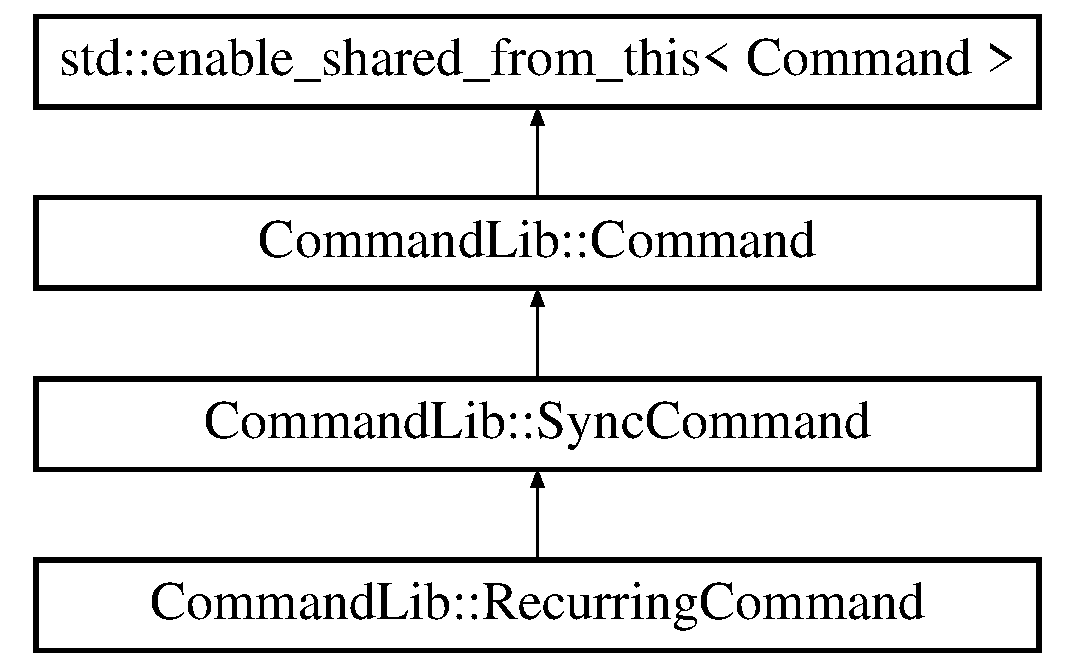
\includegraphics[height=4.000000cm]{class_command_lib_1_1_recurring_command}
\end{center}
\end{figure}
\subsection*{Classes}
\begin{DoxyCompactItemize}
\item 
class \mbox{\hyperlink{class_command_lib_1_1_recurring_command_1_1_execution_time_callback}{Execution\+Time\+Callback}}
\begin{DoxyCompactList}\small\item\em Defines at what times the underlying command executes \end{DoxyCompactList}\end{DoxyCompactItemize}
\subsection*{Public Types}
\begin{DoxyCompactItemize}
\item 
typedef std\+::shared\+\_\+ptr$<$ const \mbox{\hyperlink{class_command_lib_1_1_recurring_command}{Recurring\+Command}} $>$ \mbox{\hyperlink{class_command_lib_1_1_recurring_command_a99bd5afbc77fa5d574fd0804146f0858}{Const\+Ptr}}
\begin{DoxyCompactList}\small\item\em Shared pointer to a non-\/modifyable \mbox{\hyperlink{class_command_lib_1_1_recurring_command}{Recurring\+Command}} object\end{DoxyCompactList}\item 
typedef std\+::shared\+\_\+ptr$<$ \mbox{\hyperlink{class_command_lib_1_1_recurring_command}{Recurring\+Command}} $>$ \mbox{\hyperlink{class_command_lib_1_1_recurring_command_a458574df1804d7f1e4ba75e7aeb701e5}{Ptr}}
\begin{DoxyCompactList}\small\item\em Shared pointer to a \mbox{\hyperlink{class_command_lib_1_1_recurring_command}{Recurring\+Command}} object\end{DoxyCompactList}\end{DoxyCompactItemize}
\subsection*{Public Member Functions}
\begin{DoxyCompactItemize}
\item 
void \mbox{\hyperlink{class_command_lib_1_1_recurring_command_a11e19f7c0cbc93c33e36f6c75d858b0f}{Skip\+Current\+Wait}} ()
\begin{DoxyCompactList}\small\item\em If currently waiting until the time to next execute the command to run, skip the wait and execute the command right away.\end{DoxyCompactList}\item 
void \mbox{\hyperlink{class_command_lib_1_1_recurring_command_a954ee8723b21944ab9aa01df0740b690}{Set\+Next\+Execution\+Time}} (const std\+::chrono\+::time\+\_\+point$<$ std\+::chrono\+::system\+\_\+clock $>$ \&time)
\begin{DoxyCompactList}\small\item\em If currently waiting until the time to next execute the command to run, resets that time to the time specified. \end{DoxyCompactList}\item 
\mbox{\Hypertarget{class_command_lib_1_1_recurring_command_a4e2073b92185dd5f7b545d774afbb929}\label{class_command_lib_1_1_recurring_command_a4e2073b92185dd5f7b545d774afbb929}} 
virtual std\+::string \mbox{\hyperlink{class_command_lib_1_1_recurring_command_a4e2073b92185dd5f7b545d774afbb929}{Class\+Name}} () const override
\begin{DoxyCompactList}\small\item\em Gets the name of the runtime instance of this class. Used for logging and diagnostic purposes.  \end{DoxyCompactList}\end{DoxyCompactItemize}
\subsection*{Static Public Member Functions}
\begin{DoxyCompactItemize}
\item 
static \mbox{\hyperlink{class_command_lib_1_1_command_a3b3e4f00144373299df5c6bb1acc319d}{Ptr}} \mbox{\hyperlink{class_command_lib_1_1_recurring_command_afac0e064cbce4cea8fe5d734367b7c3a}{Create}} (\mbox{\hyperlink{class_command_lib_1_1_command_a3b3e4f00144373299df5c6bb1acc319d}{Command\+::\+Ptr}} command, \mbox{\hyperlink{class_command_lib_1_1_recurring_command_1_1_execution_time_callback}{Execution\+Time\+Callback}} $\ast$callback)
\begin{DoxyCompactList}\small\item\em Creates a \mbox{\hyperlink{class_command_lib_1_1_recurring_command}{Recurring\+Command}} object \end{DoxyCompactList}\end{DoxyCompactItemize}
\subsection*{Protected Member Functions}
\begin{DoxyCompactItemize}
\item 
\mbox{\hyperlink{class_command_lib_1_1_recurring_command_a46723429ffa56b961949931cc4e51e22}{Recurring\+Command}} (\mbox{\hyperlink{class_command_lib_1_1_command_a3b3e4f00144373299df5c6bb1acc319d}{Command\+::\+Ptr}} command, \mbox{\hyperlink{class_command_lib_1_1_recurring_command_1_1_execution_time_callback}{Execution\+Time\+Callback}} $\ast$callback)
\begin{DoxyCompactList}\small\item\em This constructor is not public so as to enforce creation using the \mbox{\hyperlink{class_command_lib_1_1_recurring_command_afac0e064cbce4cea8fe5d734367b7c3a}{Create()}} methods. \end{DoxyCompactList}\end{DoxyCompactItemize}
\subsection*{Additional Inherited Members}


\subsection{Detailed Description}
Represents a \mbox{\hyperlink{class_command_lib_1_1_command}{Command}} that repeatedly executes at times specified by the caller

If the interval between execution times is fixed, it would be simpler to use \mbox{\hyperlink{class_command_lib_1_1_periodic_command}{Periodic\+Command}} instead. 

\subsection{Member Typedef Documentation}
\mbox{\Hypertarget{class_command_lib_1_1_recurring_command_a99bd5afbc77fa5d574fd0804146f0858}\label{class_command_lib_1_1_recurring_command_a99bd5afbc77fa5d574fd0804146f0858}} 
\index{Command\+Lib\+::\+Recurring\+Command@{Command\+Lib\+::\+Recurring\+Command}!Const\+Ptr@{Const\+Ptr}}
\index{Const\+Ptr@{Const\+Ptr}!Command\+Lib\+::\+Recurring\+Command@{Command\+Lib\+::\+Recurring\+Command}}
\subsubsection{\texorpdfstring{Const\+Ptr}{ConstPtr}}
{\footnotesize\ttfamily typedef std\+::shared\+\_\+ptr$<$const \mbox{\hyperlink{class_command_lib_1_1_recurring_command}{Recurring\+Command}}$>$ \mbox{\hyperlink{class_command_lib_1_1_recurring_command_a99bd5afbc77fa5d574fd0804146f0858}{Command\+Lib\+::\+Recurring\+Command\+::\+Const\+Ptr}}}



Shared pointer to a non-\/modifyable \mbox{\hyperlink{class_command_lib_1_1_recurring_command}{Recurring\+Command}} object

\mbox{\Hypertarget{class_command_lib_1_1_recurring_command_a458574df1804d7f1e4ba75e7aeb701e5}\label{class_command_lib_1_1_recurring_command_a458574df1804d7f1e4ba75e7aeb701e5}} 
\index{Command\+Lib\+::\+Recurring\+Command@{Command\+Lib\+::\+Recurring\+Command}!Ptr@{Ptr}}
\index{Ptr@{Ptr}!Command\+Lib\+::\+Recurring\+Command@{Command\+Lib\+::\+Recurring\+Command}}
\subsubsection{\texorpdfstring{Ptr}{Ptr}}
{\footnotesize\ttfamily typedef std\+::shared\+\_\+ptr$<$\mbox{\hyperlink{class_command_lib_1_1_recurring_command}{Recurring\+Command}}$>$ \mbox{\hyperlink{class_command_lib_1_1_recurring_command_a458574df1804d7f1e4ba75e7aeb701e5}{Command\+Lib\+::\+Recurring\+Command\+::\+Ptr}}}



Shared pointer to a \mbox{\hyperlink{class_command_lib_1_1_recurring_command}{Recurring\+Command}} object



\subsection{Constructor \& Destructor Documentation}
\mbox{\Hypertarget{class_command_lib_1_1_recurring_command_a46723429ffa56b961949931cc4e51e22}\label{class_command_lib_1_1_recurring_command_a46723429ffa56b961949931cc4e51e22}} 
\index{Command\+Lib\+::\+Recurring\+Command@{Command\+Lib\+::\+Recurring\+Command}!Recurring\+Command@{Recurring\+Command}}
\index{Recurring\+Command@{Recurring\+Command}!Command\+Lib\+::\+Recurring\+Command@{Command\+Lib\+::\+Recurring\+Command}}
\subsubsection{\texorpdfstring{Recurring\+Command()}{RecurringCommand()}}
{\footnotesize\ttfamily Command\+Lib\+::\+Recurring\+Command\+::\+Recurring\+Command (\begin{DoxyParamCaption}\item[{\mbox{\hyperlink{class_command_lib_1_1_command_a3b3e4f00144373299df5c6bb1acc319d}{Command\+::\+Ptr}}}]{command,  }\item[{\mbox{\hyperlink{class_command_lib_1_1_recurring_command_1_1_execution_time_callback}{Execution\+Time\+Callback}} $\ast$}]{callback }\end{DoxyParamCaption})\hspace{0.3cm}{\ttfamily [protected]}}



This constructor is not public so as to enforce creation using the \mbox{\hyperlink{class_command_lib_1_1_recurring_command_afac0e064cbce4cea8fe5d734367b7c3a}{Create()}} methods. 



\subsection{Member Function Documentation}
\mbox{\Hypertarget{class_command_lib_1_1_recurring_command_afac0e064cbce4cea8fe5d734367b7c3a}\label{class_command_lib_1_1_recurring_command_afac0e064cbce4cea8fe5d734367b7c3a}} 
\index{Command\+Lib\+::\+Recurring\+Command@{Command\+Lib\+::\+Recurring\+Command}!Create@{Create}}
\index{Create@{Create}!Command\+Lib\+::\+Recurring\+Command@{Command\+Lib\+::\+Recurring\+Command}}
\subsubsection{\texorpdfstring{Create()}{Create()}}
{\footnotesize\ttfamily static \mbox{\hyperlink{class_command_lib_1_1_command_a3b3e4f00144373299df5c6bb1acc319d}{Ptr}} Command\+Lib\+::\+Recurring\+Command\+::\+Create (\begin{DoxyParamCaption}\item[{\mbox{\hyperlink{class_command_lib_1_1_command_a3b3e4f00144373299df5c6bb1acc319d}{Command\+::\+Ptr}}}]{command,  }\item[{\mbox{\hyperlink{class_command_lib_1_1_recurring_command_1_1_execution_time_callback}{Execution\+Time\+Callback}} $\ast$}]{callback }\end{DoxyParamCaption})\hspace{0.3cm}{\ttfamily [static]}}



Creates a \mbox{\hyperlink{class_command_lib_1_1_recurring_command}{Recurring\+Command}} object 


\begin{DoxyParams}{Parameters}
{\em command} & The command to run. This object takes ownership of the command, so the passed command must not already have an owner. \\
\hline
{\em callback} & Defines at what times the underlying command executes\\
\hline
\end{DoxyParams}
\mbox{\Hypertarget{class_command_lib_1_1_recurring_command_a954ee8723b21944ab9aa01df0740b690}\label{class_command_lib_1_1_recurring_command_a954ee8723b21944ab9aa01df0740b690}} 
\index{Command\+Lib\+::\+Recurring\+Command@{Command\+Lib\+::\+Recurring\+Command}!Set\+Next\+Execution\+Time@{Set\+Next\+Execution\+Time}}
\index{Set\+Next\+Execution\+Time@{Set\+Next\+Execution\+Time}!Command\+Lib\+::\+Recurring\+Command@{Command\+Lib\+::\+Recurring\+Command}}
\subsubsection{\texorpdfstring{Set\+Next\+Execution\+Time()}{SetNextExecutionTime()}}
{\footnotesize\ttfamily void Command\+Lib\+::\+Recurring\+Command\+::\+Set\+Next\+Execution\+Time (\begin{DoxyParamCaption}\item[{const std\+::chrono\+::time\+\_\+point$<$ std\+::chrono\+::system\+\_\+clock $>$ \&}]{time }\end{DoxyParamCaption})}



If currently waiting until the time to next execute the command to run, resets that time to the time specified. 


\begin{DoxyParams}{Parameters}
{\em time} & The time to execute the command to run. If a time in the past is specified, the command to run will execute immediately. \\
\hline
\end{DoxyParams}


This is a no-\/op if this \mbox{\hyperlink{class_command_lib_1_1_recurring_command}{Recurring\+Command}} object is not currently executing. command is executing. \mbox{\Hypertarget{class_command_lib_1_1_recurring_command_a11e19f7c0cbc93c33e36f6c75d858b0f}\label{class_command_lib_1_1_recurring_command_a11e19f7c0cbc93c33e36f6c75d858b0f}} 
\index{Command\+Lib\+::\+Recurring\+Command@{Command\+Lib\+::\+Recurring\+Command}!Skip\+Current\+Wait@{Skip\+Current\+Wait}}
\index{Skip\+Current\+Wait@{Skip\+Current\+Wait}!Command\+Lib\+::\+Recurring\+Command@{Command\+Lib\+::\+Recurring\+Command}}
\subsubsection{\texorpdfstring{Skip\+Current\+Wait()}{SkipCurrentWait()}}
{\footnotesize\ttfamily void Command\+Lib\+::\+Recurring\+Command\+::\+Skip\+Current\+Wait (\begin{DoxyParamCaption}{ }\end{DoxyParamCaption})}



If currently waiting until the time to next execute the command to run, skip the wait and execute the command right away.

This is a no-\/op if this \mbox{\hyperlink{class_command_lib_1_1_scheduled_command}{Scheduled\+Command}} object is not currently executing

The documentation for this class was generated from the following file\+:\begin{DoxyCompactItemize}
\item 
C\+:/\+Users/efieleke/\+Documents/\+Git\+Hub/\+Command\+Lib\+For\+C\+P\+P/\+Command\+Lib/include/Recurring\+Command.\+h\end{DoxyCompactItemize}

\hypertarget{class_command_lib_1_1_retryable_command}{}\doxysection{Command\+Lib\+::Retryable\+Command Class Reference}
\label{class_command_lib_1_1_retryable_command}\index{CommandLib::RetryableCommand@{CommandLib::RetryableCommand}}


This \mbox{\hyperlink{class_command_lib_1_1_command}{Command}} wraps another command, allowing the command to be retried upon failure, up to any number of times.  




{\ttfamily \#include $<$Retryable\+Command.\+h$>$}

Inheritance diagram for Command\+Lib\+::Retryable\+Command\+:\begin{figure}[H]
\begin{center}
\leavevmode
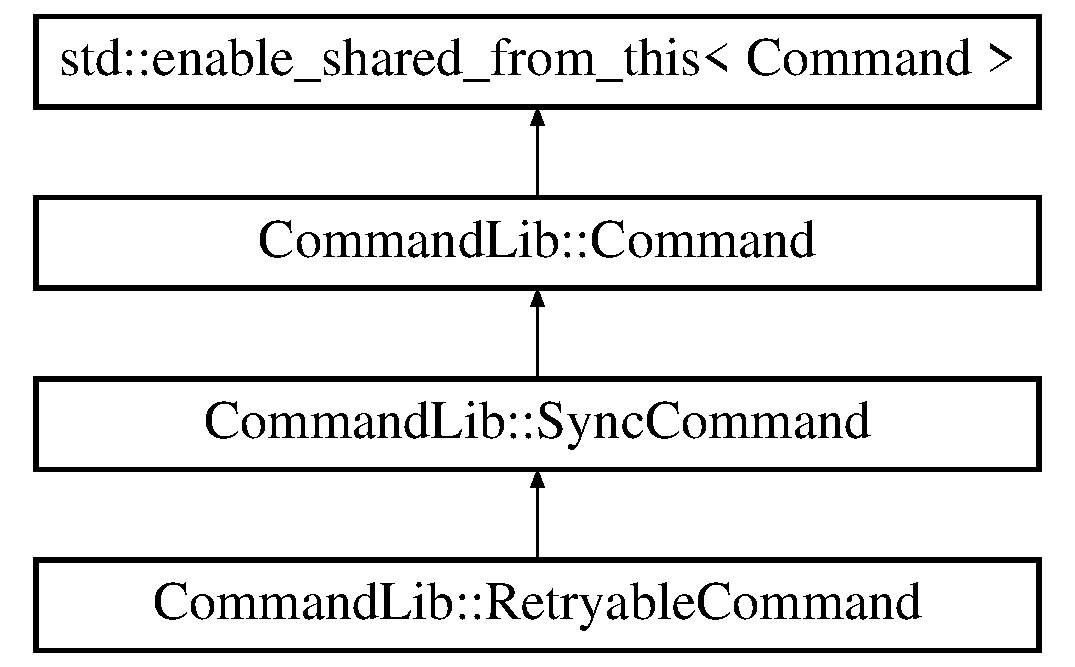
\includegraphics[height=4.000000cm]{class_command_lib_1_1_retryable_command}
\end{center}
\end{figure}
\doxysubsection*{Classes}
\begin{DoxyCompactItemize}
\item 
class \mbox{\hyperlink{class_command_lib_1_1_retryable_command_1_1_retry_callback}{Retry\+Callback}}
\begin{DoxyCompactList}\small\item\em Interface that defines aspects of retry behavior \end{DoxyCompactList}\end{DoxyCompactItemize}
\doxysubsection*{Public Types}
\begin{DoxyCompactItemize}
\item 
typedef std\+::shared\+\_\+ptr$<$ const \mbox{\hyperlink{class_command_lib_1_1_retryable_command}{Retryable\+Command}} $>$ \mbox{\hyperlink{class_command_lib_1_1_retryable_command_a8fadc39a8e4e18ddf7f468299dc55098}{Const\+Ptr}}
\begin{DoxyCompactList}\small\item\em Shared pointer to a non-\/modifyable \mbox{\hyperlink{class_command_lib_1_1_retryable_command}{Retryable\+Command}} object \end{DoxyCompactList}\item 
typedef std\+::shared\+\_\+ptr$<$ \mbox{\hyperlink{class_command_lib_1_1_retryable_command}{Retryable\+Command}} $>$ \mbox{\hyperlink{class_command_lib_1_1_retryable_command_a5bb8960c450efd6e72f93a2409c73d4c}{Ptr}}
\begin{DoxyCompactList}\small\item\em Shared pointer to a \mbox{\hyperlink{class_command_lib_1_1_retryable_command}{Retryable\+Command}} object \end{DoxyCompactList}\end{DoxyCompactItemize}
\doxysubsection*{Public Member Functions}
\begin{DoxyCompactItemize}
\item 
\mbox{\Hypertarget{class_command_lib_1_1_retryable_command_ace5c335248d89b0bf162de17a9579a74}\label{class_command_lib_1_1_retryable_command_ace5c335248d89b0bf162de17a9579a74}} 
virtual std\+::string \mbox{\hyperlink{class_command_lib_1_1_retryable_command_ace5c335248d89b0bf162de17a9579a74}{Class\+Name}} () const override
\begin{DoxyCompactList}\small\item\em Gets the name of the runtime instance of this class. Used for logging and diagnostic purposes. \end{DoxyCompactList}\end{DoxyCompactItemize}
\doxysubsection*{Static Public Member Functions}
\begin{DoxyCompactItemize}
\item 
static \mbox{\hyperlink{class_command_lib_1_1_command_a3b3e4f00144373299df5c6bb1acc319d}{Ptr}} \mbox{\hyperlink{class_command_lib_1_1_retryable_command_ae37523bf0a28f0a3ad8953a59cc1a128}{Create}} (\mbox{\hyperlink{class_command_lib_1_1_command_a3b3e4f00144373299df5c6bb1acc319d}{Command\+::\+Ptr}} command, \mbox{\hyperlink{class_command_lib_1_1_retryable_command_1_1_retry_callback}{Retry\+Callback}} $\ast$callback)
\begin{DoxyCompactList}\small\item\em Creates a \mbox{\hyperlink{class_command_lib_1_1_retryable_command}{Retryable\+Command}} \end{DoxyCompactList}\end{DoxyCompactItemize}
\doxysubsection*{Protected Member Functions}
\begin{DoxyCompactItemize}
\item 
\mbox{\hyperlink{class_command_lib_1_1_retryable_command_a0fc3a84697043a689c83106f9f9c6a4a}{Retryable\+Command}} (\mbox{\hyperlink{class_command_lib_1_1_command_a3b3e4f00144373299df5c6bb1acc319d}{Command\+::\+Ptr}} command, \mbox{\hyperlink{class_command_lib_1_1_retryable_command_1_1_retry_callback}{Retry\+Callback}} $\ast$callback)
\begin{DoxyCompactList}\small\item\em This constructor is not public so as to enforce creation using the \mbox{\hyperlink{class_command_lib_1_1_retryable_command_ae37523bf0a28f0a3ad8953a59cc1a128}{Create()}} methods. \end{DoxyCompactList}\end{DoxyCompactItemize}
\doxysubsection*{Additional Inherited Members}


\doxysubsection{Detailed Description}
This \mbox{\hyperlink{class_command_lib_1_1_command}{Command}} wraps another command, allowing the command to be retried upon failure, up to any number of times. 



\doxysubsection{Member Typedef Documentation}
\mbox{\Hypertarget{class_command_lib_1_1_retryable_command_a8fadc39a8e4e18ddf7f468299dc55098}\label{class_command_lib_1_1_retryable_command_a8fadc39a8e4e18ddf7f468299dc55098}} 
\index{CommandLib::RetryableCommand@{CommandLib::RetryableCommand}!ConstPtr@{ConstPtr}}
\index{ConstPtr@{ConstPtr}!CommandLib::RetryableCommand@{CommandLib::RetryableCommand}}
\doxysubsubsection{\texorpdfstring{ConstPtr}{ConstPtr}}
{\footnotesize\ttfamily typedef std\+::shared\+\_\+ptr$<$const \mbox{\hyperlink{class_command_lib_1_1_retryable_command}{Retryable\+Command}}$>$ \mbox{\hyperlink{class_command_lib_1_1_retryable_command_a8fadc39a8e4e18ddf7f468299dc55098}{Command\+Lib\+::\+Retryable\+Command\+::\+Const\+Ptr}}}



Shared pointer to a non-\/modifyable \mbox{\hyperlink{class_command_lib_1_1_retryable_command}{Retryable\+Command}} object 

\mbox{\Hypertarget{class_command_lib_1_1_retryable_command_a5bb8960c450efd6e72f93a2409c73d4c}\label{class_command_lib_1_1_retryable_command_a5bb8960c450efd6e72f93a2409c73d4c}} 
\index{CommandLib::RetryableCommand@{CommandLib::RetryableCommand}!Ptr@{Ptr}}
\index{Ptr@{Ptr}!CommandLib::RetryableCommand@{CommandLib::RetryableCommand}}
\doxysubsubsection{\texorpdfstring{Ptr}{Ptr}}
{\footnotesize\ttfamily typedef std\+::shared\+\_\+ptr$<$\mbox{\hyperlink{class_command_lib_1_1_retryable_command}{Retryable\+Command}}$>$ \mbox{\hyperlink{class_command_lib_1_1_retryable_command_a5bb8960c450efd6e72f93a2409c73d4c}{Command\+Lib\+::\+Retryable\+Command\+::\+Ptr}}}



Shared pointer to a \mbox{\hyperlink{class_command_lib_1_1_retryable_command}{Retryable\+Command}} object 



\doxysubsection{Constructor \& Destructor Documentation}
\mbox{\Hypertarget{class_command_lib_1_1_retryable_command_a0fc3a84697043a689c83106f9f9c6a4a}\label{class_command_lib_1_1_retryable_command_a0fc3a84697043a689c83106f9f9c6a4a}} 
\index{CommandLib::RetryableCommand@{CommandLib::RetryableCommand}!RetryableCommand@{RetryableCommand}}
\index{RetryableCommand@{RetryableCommand}!CommandLib::RetryableCommand@{CommandLib::RetryableCommand}}
\doxysubsubsection{\texorpdfstring{RetryableCommand()}{RetryableCommand()}}
{\footnotesize\ttfamily Command\+Lib\+::\+Retryable\+Command\+::\+Retryable\+Command (\begin{DoxyParamCaption}\item[{\mbox{\hyperlink{class_command_lib_1_1_command_a3b3e4f00144373299df5c6bb1acc319d}{Command\+::\+Ptr}}}]{command,  }\item[{\mbox{\hyperlink{class_command_lib_1_1_retryable_command_1_1_retry_callback}{Retry\+Callback}} $\ast$}]{callback }\end{DoxyParamCaption})\hspace{0.3cm}{\ttfamily [protected]}}



This constructor is not public so as to enforce creation using the \mbox{\hyperlink{class_command_lib_1_1_retryable_command_ae37523bf0a28f0a3ad8953a59cc1a128}{Create()}} methods. 



\doxysubsection{Member Function Documentation}
\mbox{\Hypertarget{class_command_lib_1_1_retryable_command_ae37523bf0a28f0a3ad8953a59cc1a128}\label{class_command_lib_1_1_retryable_command_ae37523bf0a28f0a3ad8953a59cc1a128}} 
\index{CommandLib::RetryableCommand@{CommandLib::RetryableCommand}!Create@{Create}}
\index{Create@{Create}!CommandLib::RetryableCommand@{CommandLib::RetryableCommand}}
\doxysubsubsection{\texorpdfstring{Create()}{Create()}}
{\footnotesize\ttfamily static \mbox{\hyperlink{class_command_lib_1_1_command_a3b3e4f00144373299df5c6bb1acc319d}{Ptr}} Command\+Lib\+::\+Retryable\+Command\+::\+Create (\begin{DoxyParamCaption}\item[{\mbox{\hyperlink{class_command_lib_1_1_command_a3b3e4f00144373299df5c6bb1acc319d}{Command\+::\+Ptr}}}]{command,  }\item[{\mbox{\hyperlink{class_command_lib_1_1_retryable_command_1_1_retry_callback}{Retry\+Callback}} $\ast$}]{callback }\end{DoxyParamCaption})\hspace{0.3cm}{\ttfamily [static]}}



Creates a \mbox{\hyperlink{class_command_lib_1_1_retryable_command}{Retryable\+Command}} 


\begin{DoxyParams}{Parameters}
{\em command} & The command to run. This object takes ownership of the command, so the passed command must not already have an owner. The passed command will be disposed when this \mbox{\hyperlink{class_command_lib_1_1_retryable_command}{Retryable\+Command}} object is disposed. \\
\hline
{\em callback} & This object defines aspects of retry behavior\\
\hline
\end{DoxyParams}


The documentation for this class was generated from the following file\+:\begin{DoxyCompactItemize}
\item 
Command\+Lib\+For\+CPP/\+Command\+Lib/include/Retryable\+Command.\+h\end{DoxyCompactItemize}

\hypertarget{class_command_lib_1_1_retryable_command_1_1_retry_callback}{}\doxysection{Command\+Lib\+::Retryable\+Command\+::Retry\+Callback Class Reference}
\label{class_command_lib_1_1_retryable_command_1_1_retry_callback}\index{CommandLib::RetryableCommand::RetryCallback@{CommandLib::RetryableCommand::RetryCallback}}


Interface that defines aspects of retry behavior  




{\ttfamily \#include $<$Retryable\+Command.\+h$>$}

\doxysubsection*{Public Member Functions}
\begin{DoxyCompactItemize}
\item 
virtual bool \mbox{\hyperlink{class_command_lib_1_1_retryable_command_1_1_retry_callback_ad207fa406f939f7253a3ee5777d5e26f}{On\+Command\+Failed}} (size\+\_\+t fail\+Number, const std\+::exception \&reason, long long $\ast$wait\+MS)=0
\begin{DoxyCompactList}\small\item\em Callback for when a command to be retried fails \end{DoxyCompactList}\end{DoxyCompactItemize}


\doxysubsection{Detailed Description}
Interface that defines aspects of retry behavior 



\doxysubsection{Member Function Documentation}
\mbox{\Hypertarget{class_command_lib_1_1_retryable_command_1_1_retry_callback_ad207fa406f939f7253a3ee5777d5e26f}\label{class_command_lib_1_1_retryable_command_1_1_retry_callback_ad207fa406f939f7253a3ee5777d5e26f}} 
\index{CommandLib::RetryableCommand::RetryCallback@{CommandLib::RetryableCommand::RetryCallback}!OnCommandFailed@{OnCommandFailed}}
\index{OnCommandFailed@{OnCommandFailed}!CommandLib::RetryableCommand::RetryCallback@{CommandLib::RetryableCommand::RetryCallback}}
\doxysubsubsection{\texorpdfstring{OnCommandFailed()}{OnCommandFailed()}}
{\footnotesize\ttfamily virtual bool Command\+Lib\+::\+Retryable\+Command\+::\+Retry\+Callback\+::\+On\+Command\+Failed (\begin{DoxyParamCaption}\item[{size\+\_\+t}]{fail\+Number,  }\item[{const std\+::exception \&}]{reason,  }\item[{long long $\ast$}]{wait\+MS }\end{DoxyParamCaption})\hspace{0.3cm}{\ttfamily [pure virtual]}}



Callback for when a command to be retried fails 


\begin{DoxyParams}{Parameters}
{\em fail\+Number} & The number of times the command has failed (including this time)\\
\hline
{\em reason} & The reason for failure.\\
\hline
{\em wait\+MS} & The number of milliseconds to wait before retrying. This value is ignored if the method returns false. \\
\hline
\end{DoxyParams}
\begin{DoxyReturn}{Returns}
false if the command should not be retried (which will propogate the exception). Otherwise true to perform a retry after the specified wait time
\end{DoxyReturn}


The documentation for this class was generated from the following file\+:\begin{DoxyCompactItemize}
\item 
C\+:/\+Users/efiel/source/repos/efieleke/\+Command\+Lib\+For\+CPP/\+Command\+Lib/include/Retryable\+Command.\+h\end{DoxyCompactItemize}

\hypertarget{class_command_lib_1_1_scheduled_command}{}\doxysection{Command\+Lib\+::Scheduled\+Command Class Reference}
\label{class_command_lib_1_1_scheduled_command}\index{CommandLib::ScheduledCommand@{CommandLib::ScheduledCommand}}


Represents a \mbox{\hyperlink{class_command_lib_1_1_command}{Command}} that executes at a given time. When a \mbox{\hyperlink{class_command_lib_1_1_scheduled_command}{Scheduled\+Command}} is executed, it will enter an efficient wait state until the time arrives at which to execute the underlying command.  




{\ttfamily \#include $<$Scheduled\+Command.\+h$>$}

Inheritance diagram for Command\+Lib\+::Scheduled\+Command\+:\begin{figure}[H]
\begin{center}
\leavevmode
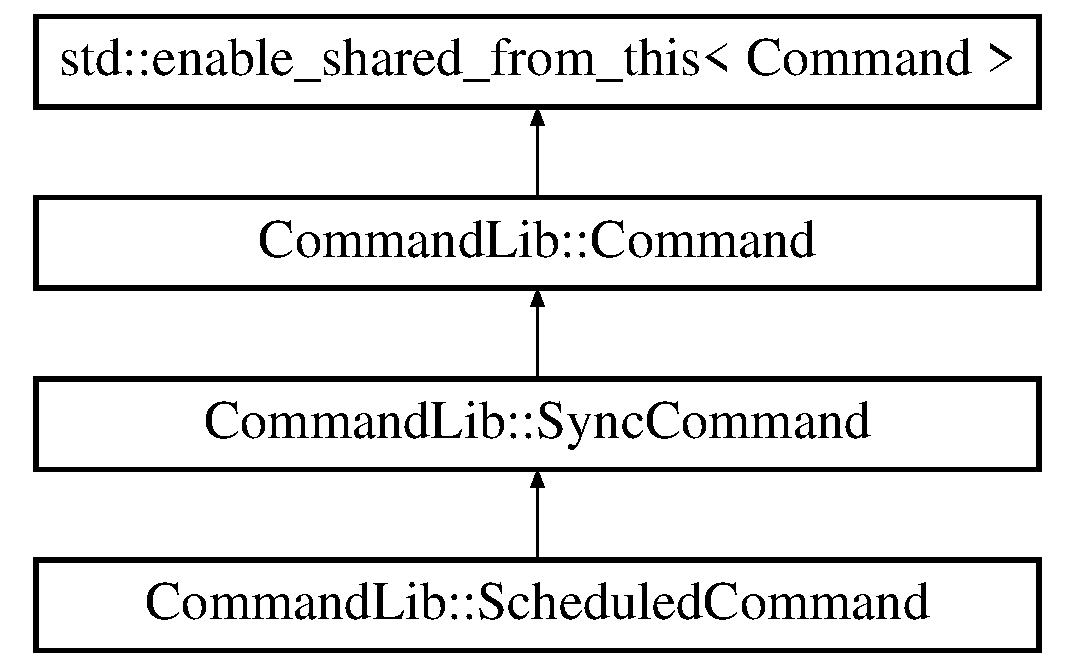
\includegraphics[height=4.000000cm]{class_command_lib_1_1_scheduled_command}
\end{center}
\end{figure}
\doxysubsection*{Public Types}
\begin{DoxyCompactItemize}
\item 
typedef std\+::shared\+\_\+ptr$<$ const \mbox{\hyperlink{class_command_lib_1_1_scheduled_command}{Scheduled\+Command}} $>$ \mbox{\hyperlink{class_command_lib_1_1_scheduled_command_a67af8cec078bd99c942eb30c60a59a33}{Const\+Ptr}}
\begin{DoxyCompactList}\small\item\em Shared pointer to a non-\/modifyable \mbox{\hyperlink{class_command_lib_1_1_scheduled_command}{Scheduled\+Command}} object \end{DoxyCompactList}\item 
typedef std\+::shared\+\_\+ptr$<$ \mbox{\hyperlink{class_command_lib_1_1_scheduled_command}{Scheduled\+Command}} $>$ \mbox{\hyperlink{class_command_lib_1_1_scheduled_command_ae5efd86637fd8da3ce36b11bc007836d}{Ptr}}
\begin{DoxyCompactList}\small\item\em Shared pointer to a \mbox{\hyperlink{class_command_lib_1_1_scheduled_command}{Scheduled\+Command}} object \end{DoxyCompactList}\end{DoxyCompactItemize}
\doxysubsection*{Public Member Functions}
\begin{DoxyCompactItemize}
\item 
std\+::chrono\+::time\+\_\+point$<$ std\+::chrono\+::system\+\_\+clock $>$ \mbox{\hyperlink{class_command_lib_1_1_scheduled_command_a283025c9c8efe2cad78a7bcdb724c614}{Get\+Time\+Of\+Execution}} () const
\begin{DoxyCompactList}\small\item\em Gets the time at which to execute the command to run \end{DoxyCompactList}\item 
void \mbox{\hyperlink{class_command_lib_1_1_scheduled_command_a12535fdcde6fe3ca5646a12b53c5302e}{Set\+Time\+Of\+Execution}} (const std\+::chrono\+::time\+\_\+point$<$ std\+::chrono\+::system\+\_\+clock $>$ \&time)
\begin{DoxyCompactList}\small\item\em Sets the time at which to execute the command to run \end{DoxyCompactList}\item 
void \mbox{\hyperlink{class_command_lib_1_1_scheduled_command_a4437a8661c9617790a032376d650e482}{Skip\+Wait}} ()
\begin{DoxyCompactList}\small\item\em Skips the current wait time before the execution of the underlying command and executes it immediately \end{DoxyCompactList}\item 
virtual std\+::string \mbox{\hyperlink{class_command_lib_1_1_scheduled_command_a3a4da8459441ce57379753e947467025}{Extended\+Description}} () const override
\begin{DoxyCompactList}\small\item\em Returns diagnostic information about this object\textquotesingle{}s state \end{DoxyCompactList}\item 
\mbox{\Hypertarget{class_command_lib_1_1_scheduled_command_ae01bdda88e63460a380579e08ced9eda}\label{class_command_lib_1_1_scheduled_command_ae01bdda88e63460a380579e08ced9eda}} 
virtual std\+::string \mbox{\hyperlink{class_command_lib_1_1_scheduled_command_ae01bdda88e63460a380579e08ced9eda}{Class\+Name}} () const override
\begin{DoxyCompactList}\small\item\em Gets the name of the runtime instance of this class. Used for logging and diagnostic purposes. \end{DoxyCompactList}\end{DoxyCompactItemize}
\doxysubsection*{Static Public Member Functions}
\begin{DoxyCompactItemize}
\item 
static \mbox{\hyperlink{class_command_lib_1_1_command_a3b3e4f00144373299df5c6bb1acc319d}{Ptr}} \mbox{\hyperlink{class_command_lib_1_1_scheduled_command_abf6008570965c8931d9c1bd8cd4f7b6a}{Create}} (\mbox{\hyperlink{class_command_lib_1_1_command_a3b3e4f00144373299df5c6bb1acc319d}{Command\+::\+Ptr}} command, const std\+::chrono\+::time\+\_\+point$<$ std\+::chrono\+::system\+\_\+clock $>$ \&time\+Of\+Execution, bool run\+Immediately\+If\+Time\+Is\+Past)
\begin{DoxyCompactList}\small\item\em Creates a \mbox{\hyperlink{class_command_lib_1_1_scheduled_command}{Scheduled\+Command}} \end{DoxyCompactList}\end{DoxyCompactItemize}
\doxysubsection*{Protected Member Functions}
\begin{DoxyCompactItemize}
\item 
\mbox{\hyperlink{class_command_lib_1_1_scheduled_command_a4f22a429c29a9e28f547f1f9f2578f93}{Scheduled\+Command}} (\mbox{\hyperlink{class_command_lib_1_1_command_a3b3e4f00144373299df5c6bb1acc319d}{Command\+::\+Ptr}} command, const std\+::chrono\+::time\+\_\+point$<$ std\+::chrono\+::system\+\_\+clock $>$ \&time\+Of\+Execution, bool run\+Immediately\+If\+Time\+Is\+Past)
\begin{DoxyCompactList}\small\item\em This constructor is not public so as to enforce creation using the \mbox{\hyperlink{class_command_lib_1_1_scheduled_command_abf6008570965c8931d9c1bd8cd4f7b6a}{Create()}} methods. \end{DoxyCompactList}\end{DoxyCompactItemize}
\doxysubsection*{Additional Inherited Members}


\doxysubsection{Detailed Description}
Represents a \mbox{\hyperlink{class_command_lib_1_1_command}{Command}} that executes at a given time. When a \mbox{\hyperlink{class_command_lib_1_1_scheduled_command}{Scheduled\+Command}} is executed, it will enter an efficient wait state until the time arrives at which to execute the underlying command. 



\doxysubsection{Member Typedef Documentation}
\mbox{\Hypertarget{class_command_lib_1_1_scheduled_command_a67af8cec078bd99c942eb30c60a59a33}\label{class_command_lib_1_1_scheduled_command_a67af8cec078bd99c942eb30c60a59a33}} 
\index{CommandLib::ScheduledCommand@{CommandLib::ScheduledCommand}!ConstPtr@{ConstPtr}}
\index{ConstPtr@{ConstPtr}!CommandLib::ScheduledCommand@{CommandLib::ScheduledCommand}}
\doxysubsubsection{\texorpdfstring{ConstPtr}{ConstPtr}}
{\footnotesize\ttfamily typedef std\+::shared\+\_\+ptr$<$const \mbox{\hyperlink{class_command_lib_1_1_scheduled_command}{Scheduled\+Command}}$>$ \mbox{\hyperlink{class_command_lib_1_1_scheduled_command_a67af8cec078bd99c942eb30c60a59a33}{Command\+Lib\+::\+Scheduled\+Command\+::\+Const\+Ptr}}}



Shared pointer to a non-\/modifyable \mbox{\hyperlink{class_command_lib_1_1_scheduled_command}{Scheduled\+Command}} object 

\mbox{\Hypertarget{class_command_lib_1_1_scheduled_command_ae5efd86637fd8da3ce36b11bc007836d}\label{class_command_lib_1_1_scheduled_command_ae5efd86637fd8da3ce36b11bc007836d}} 
\index{CommandLib::ScheduledCommand@{CommandLib::ScheduledCommand}!Ptr@{Ptr}}
\index{Ptr@{Ptr}!CommandLib::ScheduledCommand@{CommandLib::ScheduledCommand}}
\doxysubsubsection{\texorpdfstring{Ptr}{Ptr}}
{\footnotesize\ttfamily typedef std\+::shared\+\_\+ptr$<$\mbox{\hyperlink{class_command_lib_1_1_scheduled_command}{Scheduled\+Command}}$>$ \mbox{\hyperlink{class_command_lib_1_1_scheduled_command_ae5efd86637fd8da3ce36b11bc007836d}{Command\+Lib\+::\+Scheduled\+Command\+::\+Ptr}}}



Shared pointer to a \mbox{\hyperlink{class_command_lib_1_1_scheduled_command}{Scheduled\+Command}} object 



\doxysubsection{Constructor \& Destructor Documentation}
\mbox{\Hypertarget{class_command_lib_1_1_scheduled_command_a4f22a429c29a9e28f547f1f9f2578f93}\label{class_command_lib_1_1_scheduled_command_a4f22a429c29a9e28f547f1f9f2578f93}} 
\index{CommandLib::ScheduledCommand@{CommandLib::ScheduledCommand}!ScheduledCommand@{ScheduledCommand}}
\index{ScheduledCommand@{ScheduledCommand}!CommandLib::ScheduledCommand@{CommandLib::ScheduledCommand}}
\doxysubsubsection{\texorpdfstring{ScheduledCommand()}{ScheduledCommand()}}
{\footnotesize\ttfamily Command\+Lib\+::\+Scheduled\+Command\+::\+Scheduled\+Command (\begin{DoxyParamCaption}\item[{\mbox{\hyperlink{class_command_lib_1_1_command_a3b3e4f00144373299df5c6bb1acc319d}{Command\+::\+Ptr}}}]{command,  }\item[{const std\+::chrono\+::time\+\_\+point$<$ std\+::chrono\+::system\+\_\+clock $>$ \&}]{time\+Of\+Execution,  }\item[{bool}]{run\+Immediately\+If\+Time\+Is\+Past }\end{DoxyParamCaption})\hspace{0.3cm}{\ttfamily [protected]}}



This constructor is not public so as to enforce creation using the \mbox{\hyperlink{class_command_lib_1_1_scheduled_command_abf6008570965c8931d9c1bd8cd4f7b6a}{Create()}} methods. 



\doxysubsection{Member Function Documentation}
\mbox{\Hypertarget{class_command_lib_1_1_scheduled_command_abf6008570965c8931d9c1bd8cd4f7b6a}\label{class_command_lib_1_1_scheduled_command_abf6008570965c8931d9c1bd8cd4f7b6a}} 
\index{CommandLib::ScheduledCommand@{CommandLib::ScheduledCommand}!Create@{Create}}
\index{Create@{Create}!CommandLib::ScheduledCommand@{CommandLib::ScheduledCommand}}
\doxysubsubsection{\texorpdfstring{Create()}{Create()}}
{\footnotesize\ttfamily static \mbox{\hyperlink{class_command_lib_1_1_command_a3b3e4f00144373299df5c6bb1acc319d}{Ptr}} Command\+Lib\+::\+Scheduled\+Command\+::\+Create (\begin{DoxyParamCaption}\item[{\mbox{\hyperlink{class_command_lib_1_1_command_a3b3e4f00144373299df5c6bb1acc319d}{Command\+::\+Ptr}}}]{command,  }\item[{const std\+::chrono\+::time\+\_\+point$<$ std\+::chrono\+::system\+\_\+clock $>$ \&}]{time\+Of\+Execution,  }\item[{bool}]{run\+Immediately\+If\+Time\+Is\+Past }\end{DoxyParamCaption})\hspace{0.3cm}{\ttfamily [static]}}



Creates a \mbox{\hyperlink{class_command_lib_1_1_scheduled_command}{Scheduled\+Command}} 


\begin{DoxyParams}{Parameters}
{\em command} & The command to run. This object takes ownership of the command, so the passed command must not already have an owner. The passed command will be disposed when this \mbox{\hyperlink{class_command_lib_1_1_scheduled_command}{Scheduled\+Command}} object is disposed. \\
\hline
{\em time\+Of\+Execution} & The time at which to execute the command to run. Note that unless this \mbox{\hyperlink{class_command_lib_1_1_scheduled_command}{Scheduled\+Command}} object is actually executed, the command to run will never execute. \\
\hline
{\em run\+Immediately\+If\+Time\+Is\+Past} & If, when this \mbox{\hyperlink{class_command_lib_1_1_scheduled_command}{Scheduled\+Command}} is executed, the time of execution is in the past, it will execute immediately if this parameter is set to true (otherwise it will throw an Invalid\+Operation exception). \\
\hline
\end{DoxyParams}
\mbox{\Hypertarget{class_command_lib_1_1_scheduled_command_a3a4da8459441ce57379753e947467025}\label{class_command_lib_1_1_scheduled_command_a3a4da8459441ce57379753e947467025}} 
\index{CommandLib::ScheduledCommand@{CommandLib::ScheduledCommand}!ExtendedDescription@{ExtendedDescription}}
\index{ExtendedDescription@{ExtendedDescription}!CommandLib::ScheduledCommand@{CommandLib::ScheduledCommand}}
\doxysubsubsection{\texorpdfstring{ExtendedDescription()}{ExtendedDescription()}}
{\footnotesize\ttfamily virtual std\+::string Command\+Lib\+::\+Scheduled\+Command\+::\+Extended\+Description (\begin{DoxyParamCaption}{ }\end{DoxyParamCaption}) const\hspace{0.3cm}{\ttfamily [override]}, {\ttfamily [virtual]}}



Returns diagnostic information about this object\textquotesingle{}s state 

\begin{DoxyReturn}{Returns}
The returned text includes the time to execute as well as whether to run immediately if the scheduled time is in the past. 
\end{DoxyReturn}


Reimplemented from \mbox{\hyperlink{class_command_lib_1_1_command_a795a185509e7b0fc1606b3b62fe17fbb}{Command\+Lib\+::\+Command}}.

\mbox{\Hypertarget{class_command_lib_1_1_scheduled_command_a283025c9c8efe2cad78a7bcdb724c614}\label{class_command_lib_1_1_scheduled_command_a283025c9c8efe2cad78a7bcdb724c614}} 
\index{CommandLib::ScheduledCommand@{CommandLib::ScheduledCommand}!GetTimeOfExecution@{GetTimeOfExecution}}
\index{GetTimeOfExecution@{GetTimeOfExecution}!CommandLib::ScheduledCommand@{CommandLib::ScheduledCommand}}
\doxysubsubsection{\texorpdfstring{GetTimeOfExecution()}{GetTimeOfExecution()}}
{\footnotesize\ttfamily std\+::chrono\+::time\+\_\+point$<$std\+::chrono\+::system\+\_\+clock$>$ Command\+Lib\+::\+Scheduled\+Command\+::\+Get\+Time\+Of\+Execution (\begin{DoxyParamCaption}{ }\end{DoxyParamCaption}) const}



Gets the time at which to execute the command to run 

\begin{DoxyReturn}{Returns}
The time at which to execute the command to run. Note that unless this \mbox{\hyperlink{class_command_lib_1_1_scheduled_command}{Scheduled\+Command}} object is actually executed, the command to run will never execute. 
\end{DoxyReturn}
\mbox{\Hypertarget{class_command_lib_1_1_scheduled_command_a12535fdcde6fe3ca5646a12b53c5302e}\label{class_command_lib_1_1_scheduled_command_a12535fdcde6fe3ca5646a12b53c5302e}} 
\index{CommandLib::ScheduledCommand@{CommandLib::ScheduledCommand}!SetTimeOfExecution@{SetTimeOfExecution}}
\index{SetTimeOfExecution@{SetTimeOfExecution}!CommandLib::ScheduledCommand@{CommandLib::ScheduledCommand}}
\doxysubsubsection{\texorpdfstring{SetTimeOfExecution()}{SetTimeOfExecution()}}
{\footnotesize\ttfamily void Command\+Lib\+::\+Scheduled\+Command\+::\+Set\+Time\+Of\+Execution (\begin{DoxyParamCaption}\item[{const std\+::chrono\+::time\+\_\+point$<$ std\+::chrono\+::system\+\_\+clock $>$ \&}]{time }\end{DoxyParamCaption})}



Sets the time at which to execute the command to run 


\begin{DoxyParams}{Parameters}
{\em time} & The time at which to execute the command to run. Note that unless this \mbox{\hyperlink{class_command_lib_1_1_scheduled_command}{Scheduled\+Command}} object is actually executed, the command to run will never execute. \\
\hline
\end{DoxyParams}


It is safe to change this property while this command is executing, although if the underlying command to run has already begun execution, it will have no effect. \mbox{\Hypertarget{class_command_lib_1_1_scheduled_command_a4437a8661c9617790a032376d650e482}\label{class_command_lib_1_1_scheduled_command_a4437a8661c9617790a032376d650e482}} 
\index{CommandLib::ScheduledCommand@{CommandLib::ScheduledCommand}!SkipWait@{SkipWait}}
\index{SkipWait@{SkipWait}!CommandLib::ScheduledCommand@{CommandLib::ScheduledCommand}}
\doxysubsubsection{\texorpdfstring{SkipWait()}{SkipWait()}}
{\footnotesize\ttfamily void Command\+Lib\+::\+Scheduled\+Command\+::\+Skip\+Wait (\begin{DoxyParamCaption}{ }\end{DoxyParamCaption})}



Skips the current wait time before the execution of the underlying command and executes it immediately 

This is a no-\/op if this \mbox{\hyperlink{class_command_lib_1_1_scheduled_command}{Scheduled\+Command}} object is not currently executing

The documentation for this class was generated from the following file\+:\begin{DoxyCompactItemize}
\item 
Command\+Lib\+For\+CPP/\+Command\+Lib/include/Scheduled\+Command.\+h\end{DoxyCompactItemize}

\hypertarget{class_command_lib_1_1_sequential_commands}{}\section{Command\+Lib\+:\+:Sequential\+Commands Class Reference}
\label{class_command_lib_1_1_sequential_commands}\index{Command\+Lib\+::\+Sequential\+Commands@{Command\+Lib\+::\+Sequential\+Commands}}


\mbox{\hyperlink{class_command_lib_1_1_sequential_commands}{Sequential\+Commands}} is a \mbox{\hyperlink{class_command_lib_1_1_command}{Command}} object which contains a collection of commands which are run in sequence  




{\ttfamily \#include $<$Sequential\+Commands.\+h$>$}

Inheritance diagram for Command\+Lib\+:\+:Sequential\+Commands\+:\begin{figure}[H]
\begin{center}
\leavevmode
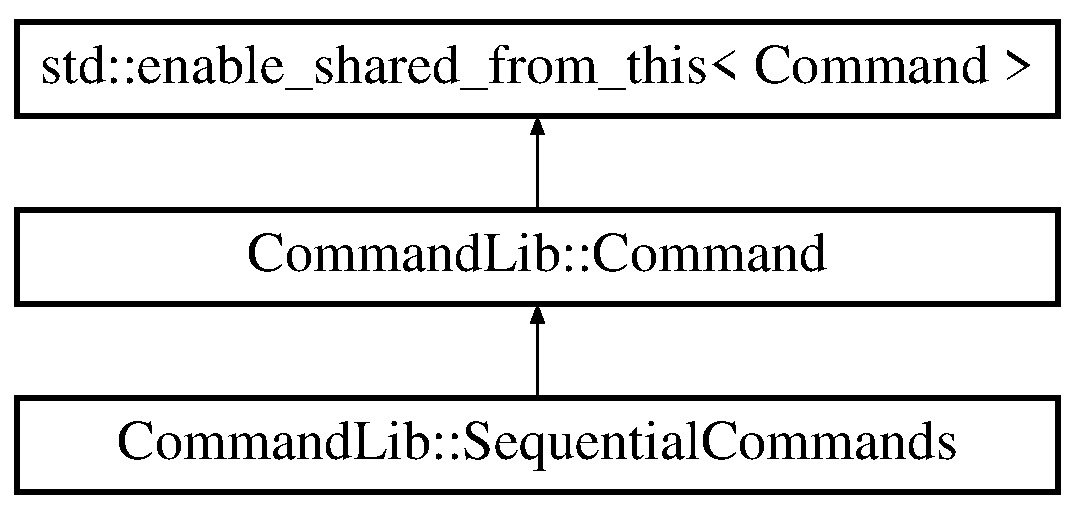
\includegraphics[height=3.000000cm]{class_command_lib_1_1_sequential_commands}
\end{center}
\end{figure}
\subsection*{Public Types}
\begin{DoxyCompactItemize}
\item 
typedef std\+::shared\+\_\+ptr$<$ const \mbox{\hyperlink{class_command_lib_1_1_sequential_commands}{Sequential\+Commands}} $>$ \mbox{\hyperlink{class_command_lib_1_1_sequential_commands_a833e8df5749f6f13b93eaa1d724799e9}{Const\+Ptr}}
\begin{DoxyCompactList}\small\item\em Shared pointer to a non-\/modifyable \mbox{\hyperlink{class_command_lib_1_1_sequential_commands}{Sequential\+Commands}} object\end{DoxyCompactList}\item 
typedef std\+::shared\+\_\+ptr$<$ \mbox{\hyperlink{class_command_lib_1_1_sequential_commands}{Sequential\+Commands}} $>$ \mbox{\hyperlink{class_command_lib_1_1_sequential_commands_adf77d8fcaebe414c283e553ba0604228}{Ptr}}
\begin{DoxyCompactList}\small\item\em Shared pointer to a \mbox{\hyperlink{class_command_lib_1_1_sequential_commands}{Sequential\+Commands}} object\end{DoxyCompactList}\end{DoxyCompactItemize}
\subsection*{Public Member Functions}
\begin{DoxyCompactItemize}
\item 
void \mbox{\hyperlink{class_command_lib_1_1_sequential_commands_af0100e15f7897471ce84802ab6c25e00}{Add}} (\mbox{\hyperlink{class_command_lib_1_1_command_a3b3e4f00144373299df5c6bb1acc319d}{Command\+::\+Ptr}} command)
\begin{DoxyCompactList}\small\item\em Adds a \mbox{\hyperlink{class_command_lib_1_1_command}{Command}} to the collection to execute.\end{DoxyCompactList}\item 
void \mbox{\hyperlink{class_command_lib_1_1_sequential_commands_ad022ea238a8c3ac1c1f71a5b71f6d94f}{Clear}} ()
\begin{DoxyCompactList}\small\item\em Empties all commands from the collection. Behavior is undefined if you call this while this command is executing. \end{DoxyCompactList}\item 
virtual std\+::string \mbox{\hyperlink{class_command_lib_1_1_sequential_commands_a8109d8d9b2c4a191cad02164ca173709}{Extended\+Description}} () const override
\begin{DoxyCompactList}\small\item\em Returns diagnostic information about this object\textquotesingle{}s state \end{DoxyCompactList}\item 
\mbox{\Hypertarget{class_command_lib_1_1_sequential_commands_abbfd93499d508c3f0d2d817bd59e7080}\label{class_command_lib_1_1_sequential_commands_abbfd93499d508c3f0d2d817bd59e7080}} 
virtual std\+::string \mbox{\hyperlink{class_command_lib_1_1_sequential_commands_abbfd93499d508c3f0d2d817bd59e7080}{Class\+Name}} () const override
\begin{DoxyCompactList}\small\item\em Gets the name of the runtime instance of this class. Used for logging and diagnostic purposes.  \end{DoxyCompactList}\item 
\mbox{\Hypertarget{class_command_lib_1_1_sequential_commands_a47c2a881bfeab639064e36d202e32e0f}\label{class_command_lib_1_1_sequential_commands_a47c2a881bfeab639064e36d202e32e0f}} 
virtual bool \mbox{\hyperlink{class_command_lib_1_1_sequential_commands_a47c2a881bfeab639064e36d202e32e0f}{Is\+Naturally\+Synchronous}} () const final
\begin{DoxyCompactList}\small\item\em Returns true if this command\textquotesingle{}s most efficient form of execution is synchronous. This information is used on occasion to determine how to best execute a command.  \end{DoxyCompactList}\end{DoxyCompactItemize}
\subsection*{Static Public Member Functions}
\begin{DoxyCompactItemize}
\item 
static \mbox{\hyperlink{class_command_lib_1_1_command_a3b3e4f00144373299df5c6bb1acc319d}{Ptr}} \mbox{\hyperlink{class_command_lib_1_1_sequential_commands_aaacdef25d7dba29bae8ff7763c55017e}{Create}} ()
\begin{DoxyCompactList}\small\item\em Creates a \mbox{\hyperlink{class_command_lib_1_1_sequential_commands}{Sequential\+Commands}} object \end{DoxyCompactList}\end{DoxyCompactItemize}
\subsection*{Protected Member Functions}
\begin{DoxyCompactItemize}
\item 
\mbox{\hyperlink{class_command_lib_1_1_sequential_commands_ab4cbf775a047942c6fce735980f19bb0}{Sequential\+Commands}} ()
\begin{DoxyCompactList}\small\item\em This constructor is not public so as to enforce creation using the \mbox{\hyperlink{class_command_lib_1_1_sequential_commands_aaacdef25d7dba29bae8ff7763c55017e}{Create()}} methods. \end{DoxyCompactList}\end{DoxyCompactItemize}
\subsection*{Additional Inherited Members}


\subsection{Detailed Description}
\mbox{\hyperlink{class_command_lib_1_1_sequential_commands}{Sequential\+Commands}} is a \mbox{\hyperlink{class_command_lib_1_1_command}{Command}} object which contains a collection of commands which are run in sequence 



\subsection{Member Typedef Documentation}
\mbox{\Hypertarget{class_command_lib_1_1_sequential_commands_a833e8df5749f6f13b93eaa1d724799e9}\label{class_command_lib_1_1_sequential_commands_a833e8df5749f6f13b93eaa1d724799e9}} 
\index{Command\+Lib\+::\+Sequential\+Commands@{Command\+Lib\+::\+Sequential\+Commands}!Const\+Ptr@{Const\+Ptr}}
\index{Const\+Ptr@{Const\+Ptr}!Command\+Lib\+::\+Sequential\+Commands@{Command\+Lib\+::\+Sequential\+Commands}}
\subsubsection{\texorpdfstring{Const\+Ptr}{ConstPtr}}
{\footnotesize\ttfamily typedef std\+::shared\+\_\+ptr$<$const \mbox{\hyperlink{class_command_lib_1_1_sequential_commands}{Sequential\+Commands}}$>$ \mbox{\hyperlink{class_command_lib_1_1_sequential_commands_a833e8df5749f6f13b93eaa1d724799e9}{Command\+Lib\+::\+Sequential\+Commands\+::\+Const\+Ptr}}}



Shared pointer to a non-\/modifyable \mbox{\hyperlink{class_command_lib_1_1_sequential_commands}{Sequential\+Commands}} object

\mbox{\Hypertarget{class_command_lib_1_1_sequential_commands_adf77d8fcaebe414c283e553ba0604228}\label{class_command_lib_1_1_sequential_commands_adf77d8fcaebe414c283e553ba0604228}} 
\index{Command\+Lib\+::\+Sequential\+Commands@{Command\+Lib\+::\+Sequential\+Commands}!Ptr@{Ptr}}
\index{Ptr@{Ptr}!Command\+Lib\+::\+Sequential\+Commands@{Command\+Lib\+::\+Sequential\+Commands}}
\subsubsection{\texorpdfstring{Ptr}{Ptr}}
{\footnotesize\ttfamily typedef std\+::shared\+\_\+ptr$<$\mbox{\hyperlink{class_command_lib_1_1_sequential_commands}{Sequential\+Commands}}$>$ \mbox{\hyperlink{class_command_lib_1_1_sequential_commands_adf77d8fcaebe414c283e553ba0604228}{Command\+Lib\+::\+Sequential\+Commands\+::\+Ptr}}}



Shared pointer to a \mbox{\hyperlink{class_command_lib_1_1_sequential_commands}{Sequential\+Commands}} object



\subsection{Constructor \& Destructor Documentation}
\mbox{\Hypertarget{class_command_lib_1_1_sequential_commands_ab4cbf775a047942c6fce735980f19bb0}\label{class_command_lib_1_1_sequential_commands_ab4cbf775a047942c6fce735980f19bb0}} 
\index{Command\+Lib\+::\+Sequential\+Commands@{Command\+Lib\+::\+Sequential\+Commands}!Sequential\+Commands@{Sequential\+Commands}}
\index{Sequential\+Commands@{Sequential\+Commands}!Command\+Lib\+::\+Sequential\+Commands@{Command\+Lib\+::\+Sequential\+Commands}}
\subsubsection{\texorpdfstring{Sequential\+Commands()}{SequentialCommands()}}
{\footnotesize\ttfamily Command\+Lib\+::\+Sequential\+Commands\+::\+Sequential\+Commands (\begin{DoxyParamCaption}{ }\end{DoxyParamCaption})\hspace{0.3cm}{\ttfamily [protected]}}



This constructor is not public so as to enforce creation using the \mbox{\hyperlink{class_command_lib_1_1_sequential_commands_aaacdef25d7dba29bae8ff7763c55017e}{Create()}} methods. 



\subsection{Member Function Documentation}
\mbox{\Hypertarget{class_command_lib_1_1_sequential_commands_af0100e15f7897471ce84802ab6c25e00}\label{class_command_lib_1_1_sequential_commands_af0100e15f7897471ce84802ab6c25e00}} 
\index{Command\+Lib\+::\+Sequential\+Commands@{Command\+Lib\+::\+Sequential\+Commands}!Add@{Add}}
\index{Add@{Add}!Command\+Lib\+::\+Sequential\+Commands@{Command\+Lib\+::\+Sequential\+Commands}}
\subsubsection{\texorpdfstring{Add()}{Add()}}
{\footnotesize\ttfamily void Command\+Lib\+::\+Sequential\+Commands\+::\+Add (\begin{DoxyParamCaption}\item[{\mbox{\hyperlink{class_command_lib_1_1_command_a3b3e4f00144373299df5c6bb1acc319d}{Command\+::\+Ptr}}}]{command }\end{DoxyParamCaption})}



Adds a \mbox{\hyperlink{class_command_lib_1_1_command}{Command}} to the collection to execute.


\begin{DoxyParams}{Parameters}
{\em command} & The command to add\\
\hline
\end{DoxyParams}


This object takes ownership of any commands that are added, so the passed command must not already have an owner. 

Behavior is undefined if you add a command while this Seqential\+Commands object is executing\mbox{\Hypertarget{class_command_lib_1_1_sequential_commands_ad022ea238a8c3ac1c1f71a5b71f6d94f}\label{class_command_lib_1_1_sequential_commands_ad022ea238a8c3ac1c1f71a5b71f6d94f}} 
\index{Command\+Lib\+::\+Sequential\+Commands@{Command\+Lib\+::\+Sequential\+Commands}!Clear@{Clear}}
\index{Clear@{Clear}!Command\+Lib\+::\+Sequential\+Commands@{Command\+Lib\+::\+Sequential\+Commands}}
\subsubsection{\texorpdfstring{Clear()}{Clear()}}
{\footnotesize\ttfamily void Command\+Lib\+::\+Sequential\+Commands\+::\+Clear (\begin{DoxyParamCaption}{ }\end{DoxyParamCaption})}



Empties all commands from the collection. Behavior is undefined if you call this while this command is executing. 

\mbox{\Hypertarget{class_command_lib_1_1_sequential_commands_aaacdef25d7dba29bae8ff7763c55017e}\label{class_command_lib_1_1_sequential_commands_aaacdef25d7dba29bae8ff7763c55017e}} 
\index{Command\+Lib\+::\+Sequential\+Commands@{Command\+Lib\+::\+Sequential\+Commands}!Create@{Create}}
\index{Create@{Create}!Command\+Lib\+::\+Sequential\+Commands@{Command\+Lib\+::\+Sequential\+Commands}}
\subsubsection{\texorpdfstring{Create()}{Create()}}
{\footnotesize\ttfamily static \mbox{\hyperlink{class_command_lib_1_1_command_a3b3e4f00144373299df5c6bb1acc319d}{Ptr}} Command\+Lib\+::\+Sequential\+Commands\+::\+Create (\begin{DoxyParamCaption}{ }\end{DoxyParamCaption})\hspace{0.3cm}{\ttfamily [static]}}



Creates a \mbox{\hyperlink{class_command_lib_1_1_sequential_commands}{Sequential\+Commands}} object 

\mbox{\Hypertarget{class_command_lib_1_1_sequential_commands_a8109d8d9b2c4a191cad02164ca173709}\label{class_command_lib_1_1_sequential_commands_a8109d8d9b2c4a191cad02164ca173709}} 
\index{Command\+Lib\+::\+Sequential\+Commands@{Command\+Lib\+::\+Sequential\+Commands}!Extended\+Description@{Extended\+Description}}
\index{Extended\+Description@{Extended\+Description}!Command\+Lib\+::\+Sequential\+Commands@{Command\+Lib\+::\+Sequential\+Commands}}
\subsubsection{\texorpdfstring{Extended\+Description()}{ExtendedDescription()}}
{\footnotesize\ttfamily virtual std\+::string Command\+Lib\+::\+Sequential\+Commands\+::\+Extended\+Description (\begin{DoxyParamCaption}{ }\end{DoxyParamCaption}) const\hspace{0.3cm}{\ttfamily [override]}, {\ttfamily [virtual]}}



Returns diagnostic information about this object\textquotesingle{}s state 

\begin{DoxyReturn}{Returns}
The returned text includes the number of commands in the collection 
\end{DoxyReturn}


Reimplemented from \mbox{\hyperlink{class_command_lib_1_1_command_a795a185509e7b0fc1606b3b62fe17fbb}{Command\+Lib\+::\+Command}}.



The documentation for this class was generated from the following file\+:\begin{DoxyCompactItemize}
\item 
C\+:/\+Users/efieleke/\+Documents/\+Git\+Hub/\+Command\+Lib\+For\+C\+P\+P/\+Command\+Lib/include/Sequential\+Commands.\+h\end{DoxyCompactItemize}

\hypertarget{class_command_lib_1_1_sync_command}{}\doxysection{Command\+Lib\+::Sync\+Command Class Reference}
\label{class_command_lib_1_1_sync_command}\index{CommandLib::SyncCommand@{CommandLib::SyncCommand}}


Represents a \mbox{\hyperlink{class_command_lib_1_1_command}{Command}} which is most naturally synchronous in its implementation. If you inherit from this class, you are responsible for implementing Command\+::\+Sync\+Exe\+Impl. This class implements Command\+::\+Async\+Execute\+Impl.  




{\ttfamily \#include $<$Sync\+Command.\+h$>$}

Inheritance diagram for Command\+Lib\+::Sync\+Command\+:\begin{figure}[H]
\begin{center}
\leavevmode
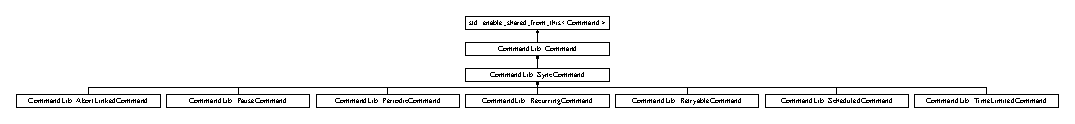
\includegraphics[height=1.216730cm]{class_command_lib_1_1_sync_command}
\end{center}
\end{figure}
\doxysubsection*{Public Member Functions}
\begin{DoxyCompactItemize}
\item 
\mbox{\Hypertarget{class_command_lib_1_1_sync_command_a7541276e393c002979ed54523116b12e}\label{class_command_lib_1_1_sync_command_a7541276e393c002979ed54523116b12e}} 
virtual bool \mbox{\hyperlink{class_command_lib_1_1_sync_command_a7541276e393c002979ed54523116b12e}{Is\+Naturally\+Synchronous}} () const final
\begin{DoxyCompactList}\small\item\em Returns true if this command\textquotesingle{}s most efficient form of execution is synchronous. This information is used on occasion to determine how to best execute a command. \end{DoxyCompactList}\end{DoxyCompactItemize}
\doxysubsection*{Additional Inherited Members}


\doxysubsection{Detailed Description}
Represents a \mbox{\hyperlink{class_command_lib_1_1_command}{Command}} which is most naturally synchronous in its implementation. If you inherit from this class, you are responsible for implementing Command\+::\+Sync\+Exe\+Impl. This class implements Command\+::\+Async\+Execute\+Impl. 



The documentation for this class was generated from the following file\+:\begin{DoxyCompactItemize}
\item 
C\+:/\+Users/efiel/source/repos/efieleke/\+Command\+Lib\+For\+CPP/\+Command\+Lib/include/Sync\+Command.\+h\end{DoxyCompactItemize}

\hypertarget{class_command_lib_1_1_time_limited_command}{}\doxysection{Command\+Lib\+::Time\+Limited\+Command Class Reference}
\label{class_command_lib_1_1_time_limited_command}\index{CommandLib::TimeLimitedCommand@{CommandLib::TimeLimitedCommand}}


This \mbox{\hyperlink{class_command_lib_1_1_command}{Command}} wraps another \mbox{\hyperlink{class_command_lib_1_1_command}{Command}}, throwing a Timeout\+Exception if a specified interval elapses before the underlying command finishes execution.  




{\ttfamily \#include $<$Time\+Limited\+Command.\+h$>$}

Inheritance diagram for Command\+Lib\+::Time\+Limited\+Command\+:\begin{figure}[H]
\begin{center}
\leavevmode
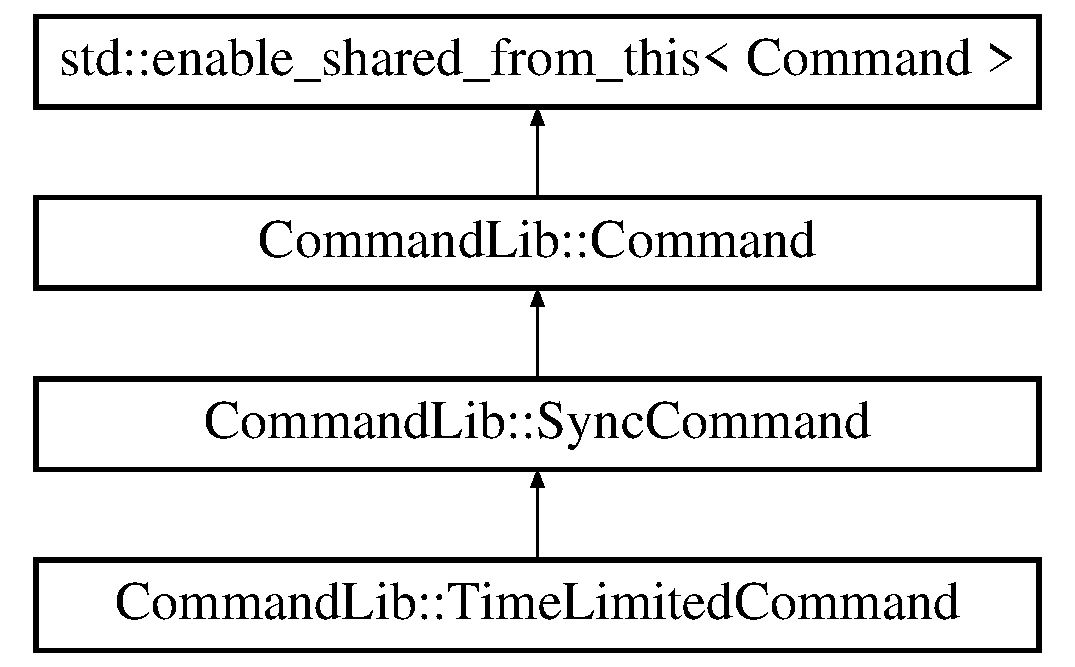
\includegraphics[height=4.000000cm]{class_command_lib_1_1_time_limited_command}
\end{center}
\end{figure}
\doxysubsection*{Public Types}
\begin{DoxyCompactItemize}
\item 
typedef std\+::shared\+\_\+ptr$<$ const \mbox{\hyperlink{class_command_lib_1_1_time_limited_command}{Time\+Limited\+Command}} $>$ \mbox{\hyperlink{class_command_lib_1_1_time_limited_command_ae2953ea50b6e131e481a2cd309b3a943}{Const\+Ptr}}
\begin{DoxyCompactList}\small\item\em Shared pointer to a non-\/modifyable \mbox{\hyperlink{class_command_lib_1_1_time_limited_command}{Time\+Limited\+Command}} object \end{DoxyCompactList}\item 
typedef std\+::shared\+\_\+ptr$<$ \mbox{\hyperlink{class_command_lib_1_1_time_limited_command}{Time\+Limited\+Command}} $>$ \mbox{\hyperlink{class_command_lib_1_1_time_limited_command_aecfced587f9da8eb1493b7bbc8759b8b}{Ptr}}
\begin{DoxyCompactList}\small\item\em Shared pointer to a \mbox{\hyperlink{class_command_lib_1_1_time_limited_command}{Time\+Limited\+Command}} object \end{DoxyCompactList}\end{DoxyCompactItemize}
\doxysubsection*{Public Member Functions}
\begin{DoxyCompactItemize}
\item 
virtual std\+::string \mbox{\hyperlink{class_command_lib_1_1_time_limited_command_aaf7018c66b91a5d1a519325b99dc3f55}{Extended\+Description}} () const override
\begin{DoxyCompactList}\small\item\em Returns diagnostic information about this object\textquotesingle{}s state \end{DoxyCompactList}\item 
\mbox{\Hypertarget{class_command_lib_1_1_time_limited_command_a2a5063ef124f555229b90f7bd82f362e}\label{class_command_lib_1_1_time_limited_command_a2a5063ef124f555229b90f7bd82f362e}} 
virtual std\+::string \mbox{\hyperlink{class_command_lib_1_1_time_limited_command_a2a5063ef124f555229b90f7bd82f362e}{Class\+Name}} () const override
\begin{DoxyCompactList}\small\item\em Gets the name of the runtime instance of this class. Used for logging and diagnostic purposes. \end{DoxyCompactList}\end{DoxyCompactItemize}
\doxysubsection*{Static Public Member Functions}
\begin{DoxyCompactItemize}
\item 
static \mbox{\hyperlink{class_command_lib_1_1_command_a3b3e4f00144373299df5c6bb1acc319d}{Ptr}} \mbox{\hyperlink{class_command_lib_1_1_time_limited_command_a7b8515c4f2780c7f5d8bc942affbc12b}{Create}} (\mbox{\hyperlink{class_command_lib_1_1_command_a3b3e4f00144373299df5c6bb1acc319d}{Command\+::\+Ptr}} command\+To\+Run, long long timeout\+MS)
\begin{DoxyCompactList}\small\item\em Creates a \mbox{\hyperlink{class_command_lib_1_1_time_limited_command}{Time\+Limited\+Command}} object \end{DoxyCompactList}\item 
{\footnotesize template$<$typename Rep , typename Period $>$ }\\static \mbox{\hyperlink{class_command_lib_1_1_command_a3b3e4f00144373299df5c6bb1acc319d}{Ptr}} \mbox{\hyperlink{class_command_lib_1_1_time_limited_command_a14e7e2915d660199c4433972a93515e7}{Create}} (\mbox{\hyperlink{class_command_lib_1_1_command_a3b3e4f00144373299df5c6bb1acc319d}{Command\+::\+Ptr}} command\+To\+Run, const std\+::chrono\+::duration$<$ Rep, Period $>$ \&timeout)
\begin{DoxyCompactList}\small\item\em Creates a \mbox{\hyperlink{class_command_lib_1_1_time_limited_command}{Time\+Limited\+Command}} object \end{DoxyCompactList}\end{DoxyCompactItemize}
\doxysubsection*{Protected Member Functions}
\begin{DoxyCompactItemize}
\item 
\mbox{\hyperlink{class_command_lib_1_1_time_limited_command_a923ec27a5e32db08d1fc3a90f73160cb}{Time\+Limited\+Command}} (long long timeout\+MS, \mbox{\hyperlink{class_command_lib_1_1_command_a3b3e4f00144373299df5c6bb1acc319d}{Command\+::\+Ptr}} command\+To\+Run)
\begin{DoxyCompactList}\small\item\em This constructor is not public so as to enforce creation using the \mbox{\hyperlink{class_command_lib_1_1_time_limited_command_a7b8515c4f2780c7f5d8bc942affbc12b}{Create()}} methods. \end{DoxyCompactList}\end{DoxyCompactItemize}
\doxysubsection*{Additional Inherited Members}


\doxysubsection{Detailed Description}
This \mbox{\hyperlink{class_command_lib_1_1_command}{Command}} wraps another \mbox{\hyperlink{class_command_lib_1_1_command}{Command}}, throwing a Timeout\+Exception if a specified interval elapses before the underlying command finishes execution. 

The underlying command to execute must be responsive to abort requests in order for the timeout interval to be honored. 

\doxysubsection{Member Typedef Documentation}
\mbox{\Hypertarget{class_command_lib_1_1_time_limited_command_ae2953ea50b6e131e481a2cd309b3a943}\label{class_command_lib_1_1_time_limited_command_ae2953ea50b6e131e481a2cd309b3a943}} 
\index{CommandLib::TimeLimitedCommand@{CommandLib::TimeLimitedCommand}!ConstPtr@{ConstPtr}}
\index{ConstPtr@{ConstPtr}!CommandLib::TimeLimitedCommand@{CommandLib::TimeLimitedCommand}}
\doxysubsubsection{\texorpdfstring{ConstPtr}{ConstPtr}}
{\footnotesize\ttfamily typedef std\+::shared\+\_\+ptr$<$const \mbox{\hyperlink{class_command_lib_1_1_time_limited_command}{Time\+Limited\+Command}}$>$ \mbox{\hyperlink{class_command_lib_1_1_time_limited_command_ae2953ea50b6e131e481a2cd309b3a943}{Command\+Lib\+::\+Time\+Limited\+Command\+::\+Const\+Ptr}}}



Shared pointer to a non-\/modifyable \mbox{\hyperlink{class_command_lib_1_1_time_limited_command}{Time\+Limited\+Command}} object 

\mbox{\Hypertarget{class_command_lib_1_1_time_limited_command_aecfced587f9da8eb1493b7bbc8759b8b}\label{class_command_lib_1_1_time_limited_command_aecfced587f9da8eb1493b7bbc8759b8b}} 
\index{CommandLib::TimeLimitedCommand@{CommandLib::TimeLimitedCommand}!Ptr@{Ptr}}
\index{Ptr@{Ptr}!CommandLib::TimeLimitedCommand@{CommandLib::TimeLimitedCommand}}
\doxysubsubsection{\texorpdfstring{Ptr}{Ptr}}
{\footnotesize\ttfamily typedef std\+::shared\+\_\+ptr$<$\mbox{\hyperlink{class_command_lib_1_1_time_limited_command}{Time\+Limited\+Command}}$>$ \mbox{\hyperlink{class_command_lib_1_1_time_limited_command_aecfced587f9da8eb1493b7bbc8759b8b}{Command\+Lib\+::\+Time\+Limited\+Command\+::\+Ptr}}}



Shared pointer to a \mbox{\hyperlink{class_command_lib_1_1_time_limited_command}{Time\+Limited\+Command}} object 



\doxysubsection{Constructor \& Destructor Documentation}
\mbox{\Hypertarget{class_command_lib_1_1_time_limited_command_a923ec27a5e32db08d1fc3a90f73160cb}\label{class_command_lib_1_1_time_limited_command_a923ec27a5e32db08d1fc3a90f73160cb}} 
\index{CommandLib::TimeLimitedCommand@{CommandLib::TimeLimitedCommand}!TimeLimitedCommand@{TimeLimitedCommand}}
\index{TimeLimitedCommand@{TimeLimitedCommand}!CommandLib::TimeLimitedCommand@{CommandLib::TimeLimitedCommand}}
\doxysubsubsection{\texorpdfstring{TimeLimitedCommand()}{TimeLimitedCommand()}}
{\footnotesize\ttfamily Command\+Lib\+::\+Time\+Limited\+Command\+::\+Time\+Limited\+Command (\begin{DoxyParamCaption}\item[{long long}]{timeout\+MS,  }\item[{\mbox{\hyperlink{class_command_lib_1_1_command_a3b3e4f00144373299df5c6bb1acc319d}{Command\+::\+Ptr}}}]{command\+To\+Run }\end{DoxyParamCaption})\hspace{0.3cm}{\ttfamily [explicit]}, {\ttfamily [protected]}}



This constructor is not public so as to enforce creation using the \mbox{\hyperlink{class_command_lib_1_1_time_limited_command_a7b8515c4f2780c7f5d8bc942affbc12b}{Create()}} methods. 



\doxysubsection{Member Function Documentation}
\mbox{\Hypertarget{class_command_lib_1_1_time_limited_command_a14e7e2915d660199c4433972a93515e7}\label{class_command_lib_1_1_time_limited_command_a14e7e2915d660199c4433972a93515e7}} 
\index{CommandLib::TimeLimitedCommand@{CommandLib::TimeLimitedCommand}!Create@{Create}}
\index{Create@{Create}!CommandLib::TimeLimitedCommand@{CommandLib::TimeLimitedCommand}}
\doxysubsubsection{\texorpdfstring{Create()}{Create()}\hspace{0.1cm}{\footnotesize\ttfamily [1/2]}}
{\footnotesize\ttfamily template$<$typename Rep , typename Period $>$ \\
static \mbox{\hyperlink{class_command_lib_1_1_command_a3b3e4f00144373299df5c6bb1acc319d}{Ptr}} Command\+Lib\+::\+Time\+Limited\+Command\+::\+Create (\begin{DoxyParamCaption}\item[{\mbox{\hyperlink{class_command_lib_1_1_command_a3b3e4f00144373299df5c6bb1acc319d}{Command\+::\+Ptr}}}]{command\+To\+Run,  }\item[{const std\+::chrono\+::duration$<$ Rep, Period $>$ \&}]{timeout }\end{DoxyParamCaption})\hspace{0.3cm}{\ttfamily [inline]}, {\ttfamily [static]}}



Creates a \mbox{\hyperlink{class_command_lib_1_1_time_limited_command}{Time\+Limited\+Command}} object 


\begin{DoxyParams}{Parameters}
{\em command\+To\+Run} & The command to run. This object takes ownership of the command, so the passed command must not already have an owner. \\
\hline
{\em timeout} & The timeout interval. The countdown does not begin until this command is executed. \\
\hline
\end{DoxyParams}
\mbox{\Hypertarget{class_command_lib_1_1_time_limited_command_a7b8515c4f2780c7f5d8bc942affbc12b}\label{class_command_lib_1_1_time_limited_command_a7b8515c4f2780c7f5d8bc942affbc12b}} 
\index{CommandLib::TimeLimitedCommand@{CommandLib::TimeLimitedCommand}!Create@{Create}}
\index{Create@{Create}!CommandLib::TimeLimitedCommand@{CommandLib::TimeLimitedCommand}}
\doxysubsubsection{\texorpdfstring{Create()}{Create()}\hspace{0.1cm}{\footnotesize\ttfamily [2/2]}}
{\footnotesize\ttfamily static \mbox{\hyperlink{class_command_lib_1_1_command_a3b3e4f00144373299df5c6bb1acc319d}{Ptr}} Command\+Lib\+::\+Time\+Limited\+Command\+::\+Create (\begin{DoxyParamCaption}\item[{\mbox{\hyperlink{class_command_lib_1_1_command_a3b3e4f00144373299df5c6bb1acc319d}{Command\+::\+Ptr}}}]{command\+To\+Run,  }\item[{long long}]{timeout\+MS }\end{DoxyParamCaption})\hspace{0.3cm}{\ttfamily [static]}}



Creates a \mbox{\hyperlink{class_command_lib_1_1_time_limited_command}{Time\+Limited\+Command}} object 


\begin{DoxyParams}{Parameters}
{\em command\+To\+Run} & The command to run. This object takes ownership of the command, so the passed command must not already have an owner. \\
\hline
{\em timeout\+MS} & The timeout interval, in milliseconds. The countdown does not begin until this command is executed. \\
\hline
\end{DoxyParams}
\mbox{\Hypertarget{class_command_lib_1_1_time_limited_command_aaf7018c66b91a5d1a519325b99dc3f55}\label{class_command_lib_1_1_time_limited_command_aaf7018c66b91a5d1a519325b99dc3f55}} 
\index{CommandLib::TimeLimitedCommand@{CommandLib::TimeLimitedCommand}!ExtendedDescription@{ExtendedDescription}}
\index{ExtendedDescription@{ExtendedDescription}!CommandLib::TimeLimitedCommand@{CommandLib::TimeLimitedCommand}}
\doxysubsubsection{\texorpdfstring{ExtendedDescription()}{ExtendedDescription()}}
{\footnotesize\ttfamily virtual std\+::string Command\+Lib\+::\+Time\+Limited\+Command\+::\+Extended\+Description (\begin{DoxyParamCaption}{ }\end{DoxyParamCaption}) const\hspace{0.3cm}{\ttfamily [override]}, {\ttfamily [virtual]}}



Returns diagnostic information about this object\textquotesingle{}s state 

\begin{DoxyReturn}{Returns}
The returned text includes the timeout duration. 
\end{DoxyReturn}


Reimplemented from \mbox{\hyperlink{class_command_lib_1_1_command_a795a185509e7b0fc1606b3b62fe17fbb}{Command\+Lib\+::\+Command}}.



The documentation for this class was generated from the following file\+:\begin{DoxyCompactItemize}
\item 
C\+:/\+Users/efiel/source/repos/efieleke/\+Command\+Lib\+For\+CPP/\+Command\+Lib/include/Time\+Limited\+Command.\+h\end{DoxyCompactItemize}

\hypertarget{class_command_lib_1_1_waitable}{}\doxysection{Command\+Lib\+::Waitable Class Reference}
\label{class_command_lib_1_1_waitable}\index{CommandLib::Waitable@{CommandLib::Waitable}}


This class represents an object that can be waited upon until it enters a signaled state. The reason for its existence is so that it can be added to a \mbox{\hyperlink{class_command_lib_1_1_wait_group}{Wait\+Group}} object, thus allowing a wait for multiple objects (a feature available in Windows but not in other operating systems).  




{\ttfamily \#include $<$Waitable.\+h$>$}

Inheritance diagram for Command\+Lib\+::Waitable\+:\begin{figure}[H]
\begin{center}
\leavevmode
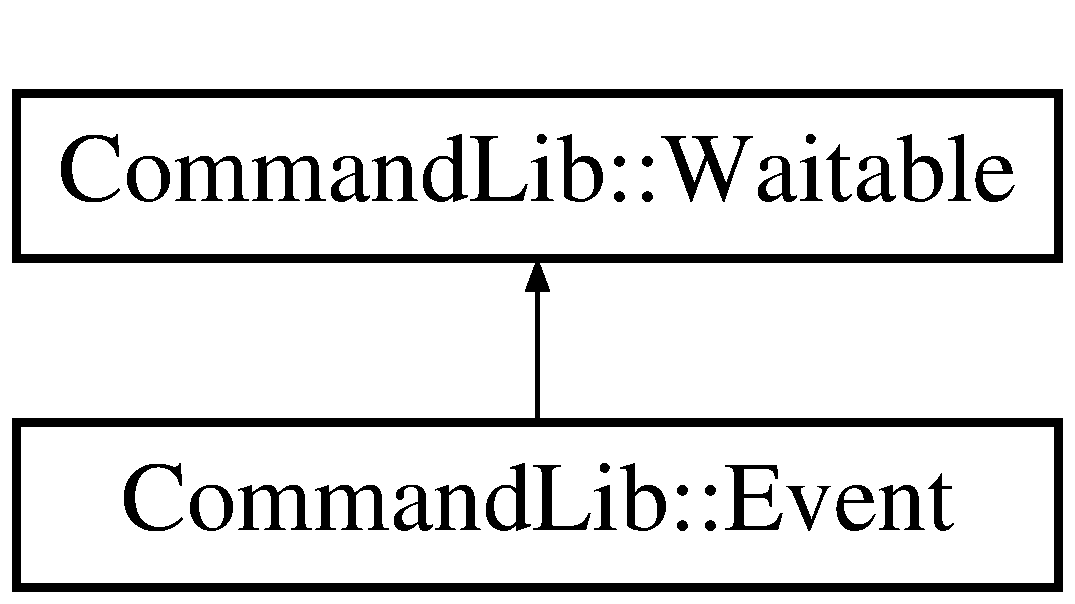
\includegraphics[height=2.000000cm]{class_command_lib_1_1_waitable}
\end{center}
\end{figure}
\doxysubsection*{Public Types}
\begin{DoxyCompactItemize}
\item 
typedef std\+::shared\+\_\+ptr$<$ const \mbox{\hyperlink{class_command_lib_1_1_waitable}{Waitable}} $>$ \mbox{\hyperlink{class_command_lib_1_1_waitable_a2b2652c778560613f9e7dd93be596387}{Const\+Ptr}}
\begin{DoxyCompactList}\small\item\em Shared pointer to a non-\/modifyable \mbox{\hyperlink{class_command_lib_1_1_waitable}{Waitable}} object \end{DoxyCompactList}\item 
typedef std\+::shared\+\_\+ptr$<$ \mbox{\hyperlink{class_command_lib_1_1_waitable}{Waitable}} $>$ \mbox{\hyperlink{class_command_lib_1_1_waitable_ac74b6b91e48220146eada76a31cf2d9b}{Ptr}}
\begin{DoxyCompactList}\small\item\em Shared pointer to a \mbox{\hyperlink{class_command_lib_1_1_waitable}{Waitable}} object \end{DoxyCompactList}\end{DoxyCompactItemize}
\doxysubsection*{Public Member Functions}
\begin{DoxyCompactItemize}
\item 
bool \mbox{\hyperlink{class_command_lib_1_1_waitable_afa4d25c0eb13db4222575f95036fbb22}{Add\+Listener}} (std\+::shared\+\_\+ptr$<$ \mbox{\hyperlink{class_command_lib_1_1_wait_monitor}{Wait\+Monitor}} $>$ listener)
\begin{DoxyCompactList}\small\item\em Add a listener for when this object becomes signaled \end{DoxyCompactList}\item 
bool \mbox{\hyperlink{class_command_lib_1_1_waitable_a4fcc6b508053a565565bc4fb591b7cf9}{Remove\+Listener}} (std\+::shared\+\_\+ptr$<$ \mbox{\hyperlink{class_command_lib_1_1_wait_monitor}{Wait\+Monitor}} $>$ listener)
\begin{DoxyCompactList}\small\item\em Removes the listener for when this object becomes signaled \end{DoxyCompactList}\item 
virtual bool \mbox{\hyperlink{class_command_lib_1_1_waitable_ac14826c4ad004a59113899b7a3f3ebcf}{Is\+Signaled}} () const =0
\begin{DoxyCompactList}\small\item\em Indicates whether or not this object is in a signaled state \end{DoxyCompactList}\item 
virtual void \mbox{\hyperlink{class_command_lib_1_1_waitable_aa3916ede3b2ca9bed013a4e256e081da}{Wait}} () const =0
\begin{DoxyCompactList}\small\item\em Waits until this object is in a signaled state \end{DoxyCompactList}\item 
virtual bool \mbox{\hyperlink{class_command_lib_1_1_waitable_ad5f9233b05a3ca2bce4ec572bfb82f4b}{Wait}} (long long ms) const =0
\begin{DoxyCompactList}\small\item\em Waits the given milliseconds until this object is in a signaled state \end{DoxyCompactList}\item 
{\footnotesize template$<$typename Rep , typename Period $>$ }\\bool \mbox{\hyperlink{class_command_lib_1_1_waitable_a798d6d18990d625773e0565acaa89fe3}{Wait\+For}} (const std\+::chrono\+::duration$<$ Rep, Period $>$ \&dur) const
\begin{DoxyCompactList}\small\item\em Waits the given duration until this object is in a signaled state \end{DoxyCompactList}\end{DoxyCompactItemize}
\doxysubsection*{Protected Member Functions}
\begin{DoxyCompactItemize}
\item 
void \mbox{\hyperlink{class_command_lib_1_1_waitable_a3ea1f52b7ee42671a441b531e4d3cd34}{Notify\+Listeners}} ()
\begin{DoxyCompactList}\small\item\em Implementations should call this when this object is signaled \end{DoxyCompactList}\end{DoxyCompactItemize}


\doxysubsection{Detailed Description}
This class represents an object that can be waited upon until it enters a signaled state. The reason for its existence is so that it can be added to a \mbox{\hyperlink{class_command_lib_1_1_wait_group}{Wait\+Group}} object, thus allowing a wait for multiple objects (a feature available in Windows but not in other operating systems). 



\doxysubsection{Member Typedef Documentation}
\mbox{\Hypertarget{class_command_lib_1_1_waitable_a2b2652c778560613f9e7dd93be596387}\label{class_command_lib_1_1_waitable_a2b2652c778560613f9e7dd93be596387}} 
\index{CommandLib::Waitable@{CommandLib::Waitable}!ConstPtr@{ConstPtr}}
\index{ConstPtr@{ConstPtr}!CommandLib::Waitable@{CommandLib::Waitable}}
\doxysubsubsection{\texorpdfstring{ConstPtr}{ConstPtr}}
{\footnotesize\ttfamily typedef std\+::shared\+\_\+ptr$<$const \mbox{\hyperlink{class_command_lib_1_1_waitable}{Waitable}}$>$ \mbox{\hyperlink{class_command_lib_1_1_waitable_a2b2652c778560613f9e7dd93be596387}{Command\+Lib\+::\+Waitable\+::\+Const\+Ptr}}}



Shared pointer to a non-\/modifyable \mbox{\hyperlink{class_command_lib_1_1_waitable}{Waitable}} object 

\mbox{\Hypertarget{class_command_lib_1_1_waitable_ac74b6b91e48220146eada76a31cf2d9b}\label{class_command_lib_1_1_waitable_ac74b6b91e48220146eada76a31cf2d9b}} 
\index{CommandLib::Waitable@{CommandLib::Waitable}!Ptr@{Ptr}}
\index{Ptr@{Ptr}!CommandLib::Waitable@{CommandLib::Waitable}}
\doxysubsubsection{\texorpdfstring{Ptr}{Ptr}}
{\footnotesize\ttfamily typedef std\+::shared\+\_\+ptr$<$\mbox{\hyperlink{class_command_lib_1_1_waitable}{Waitable}}$>$ \mbox{\hyperlink{class_command_lib_1_1_waitable_ac74b6b91e48220146eada76a31cf2d9b}{Command\+Lib\+::\+Waitable\+::\+Ptr}}}



Shared pointer to a \mbox{\hyperlink{class_command_lib_1_1_waitable}{Waitable}} object 



\doxysubsection{Member Function Documentation}
\mbox{\Hypertarget{class_command_lib_1_1_waitable_afa4d25c0eb13db4222575f95036fbb22}\label{class_command_lib_1_1_waitable_afa4d25c0eb13db4222575f95036fbb22}} 
\index{CommandLib::Waitable@{CommandLib::Waitable}!AddListener@{AddListener}}
\index{AddListener@{AddListener}!CommandLib::Waitable@{CommandLib::Waitable}}
\doxysubsubsection{\texorpdfstring{AddListener()}{AddListener()}}
{\footnotesize\ttfamily bool Command\+Lib\+::\+Waitable\+::\+Add\+Listener (\begin{DoxyParamCaption}\item[{std\+::shared\+\_\+ptr$<$ \mbox{\hyperlink{class_command_lib_1_1_wait_monitor}{Wait\+Monitor}} $>$}]{listener }\end{DoxyParamCaption})}



Add a listener for when this object becomes signaled 


\begin{DoxyParams}{Parameters}
{\em listener} & The listener to add\\
\hline
\end{DoxyParams}


This method is thread safe\mbox{\Hypertarget{class_command_lib_1_1_waitable_ac14826c4ad004a59113899b7a3f3ebcf}\label{class_command_lib_1_1_waitable_ac14826c4ad004a59113899b7a3f3ebcf}} 
\index{CommandLib::Waitable@{CommandLib::Waitable}!IsSignaled@{IsSignaled}}
\index{IsSignaled@{IsSignaled}!CommandLib::Waitable@{CommandLib::Waitable}}
\doxysubsubsection{\texorpdfstring{IsSignaled()}{IsSignaled()}}
{\footnotesize\ttfamily virtual bool Command\+Lib\+::\+Waitable\+::\+Is\+Signaled (\begin{DoxyParamCaption}{ }\end{DoxyParamCaption}) const\hspace{0.3cm}{\ttfamily [pure virtual]}}



Indicates whether or not this object is in a signaled state 

\begin{DoxyReturn}{Returns}
true if this object is signaled
\end{DoxyReturn}


Implemented in \mbox{\hyperlink{class_command_lib_1_1_event_a943dcf40e6b9fa09df19cd3fa870788e}{Command\+Lib\+::\+Event}}.

\mbox{\Hypertarget{class_command_lib_1_1_waitable_a3ea1f52b7ee42671a441b531e4d3cd34}\label{class_command_lib_1_1_waitable_a3ea1f52b7ee42671a441b531e4d3cd34}} 
\index{CommandLib::Waitable@{CommandLib::Waitable}!NotifyListeners@{NotifyListeners}}
\index{NotifyListeners@{NotifyListeners}!CommandLib::Waitable@{CommandLib::Waitable}}
\doxysubsubsection{\texorpdfstring{NotifyListeners()}{NotifyListeners()}}
{\footnotesize\ttfamily void Command\+Lib\+::\+Waitable\+::\+Notify\+Listeners (\begin{DoxyParamCaption}{ }\end{DoxyParamCaption})\hspace{0.3cm}{\ttfamily [protected]}}



Implementations should call this when this object is signaled 

\mbox{\Hypertarget{class_command_lib_1_1_waitable_a4fcc6b508053a565565bc4fb591b7cf9}\label{class_command_lib_1_1_waitable_a4fcc6b508053a565565bc4fb591b7cf9}} 
\index{CommandLib::Waitable@{CommandLib::Waitable}!RemoveListener@{RemoveListener}}
\index{RemoveListener@{RemoveListener}!CommandLib::Waitable@{CommandLib::Waitable}}
\doxysubsubsection{\texorpdfstring{RemoveListener()}{RemoveListener()}}
{\footnotesize\ttfamily bool Command\+Lib\+::\+Waitable\+::\+Remove\+Listener (\begin{DoxyParamCaption}\item[{std\+::shared\+\_\+ptr$<$ \mbox{\hyperlink{class_command_lib_1_1_wait_monitor}{Wait\+Monitor}} $>$}]{listener }\end{DoxyParamCaption})}



Removes the listener for when this object becomes signaled 


\begin{DoxyParams}{Parameters}
{\em listener} & The listener to remove\\
\hline
\end{DoxyParams}


This method is thread safe\mbox{\Hypertarget{class_command_lib_1_1_waitable_aa3916ede3b2ca9bed013a4e256e081da}\label{class_command_lib_1_1_waitable_aa3916ede3b2ca9bed013a4e256e081da}} 
\index{CommandLib::Waitable@{CommandLib::Waitable}!Wait@{Wait}}
\index{Wait@{Wait}!CommandLib::Waitable@{CommandLib::Waitable}}
\doxysubsubsection{\texorpdfstring{Wait()}{Wait()}\hspace{0.1cm}{\footnotesize\ttfamily [1/2]}}
{\footnotesize\ttfamily virtual void Command\+Lib\+::\+Waitable\+::\+Wait (\begin{DoxyParamCaption}{ }\end{DoxyParamCaption}) const\hspace{0.3cm}{\ttfamily [pure virtual]}}



Waits until this object is in a signaled state 

This will return immediately if this object is currently signaled 

Implemented in \mbox{\hyperlink{class_command_lib_1_1_event_a26986edd42eaa6b85b5a4ddc32af60ae}{Command\+Lib\+::\+Event}}.

\mbox{\Hypertarget{class_command_lib_1_1_waitable_ad5f9233b05a3ca2bce4ec572bfb82f4b}\label{class_command_lib_1_1_waitable_ad5f9233b05a3ca2bce4ec572bfb82f4b}} 
\index{CommandLib::Waitable@{CommandLib::Waitable}!Wait@{Wait}}
\index{Wait@{Wait}!CommandLib::Waitable@{CommandLib::Waitable}}
\doxysubsubsection{\texorpdfstring{Wait()}{Wait()}\hspace{0.1cm}{\footnotesize\ttfamily [2/2]}}
{\footnotesize\ttfamily virtual bool Command\+Lib\+::\+Waitable\+::\+Wait (\begin{DoxyParamCaption}\item[{long long}]{ms }\end{DoxyParamCaption}) const\hspace{0.3cm}{\ttfamily [pure virtual]}}



Waits the given milliseconds until this object is in a signaled state 


\begin{DoxyParams}{Parameters}
{\em ms} & The number of milliseconds to wait\\
\hline
\end{DoxyParams}
\begin{DoxyReturn}{Returns}
true if this object became signaled before the wait time elapsed, false otherwise
\end{DoxyReturn}


This will return immediately if this object is currently signaled. 

Implemented in \mbox{\hyperlink{class_command_lib_1_1_event_a395777fd83828fea3d225b2c192d70dd}{Command\+Lib\+::\+Event}}.

\mbox{\Hypertarget{class_command_lib_1_1_waitable_a798d6d18990d625773e0565acaa89fe3}\label{class_command_lib_1_1_waitable_a798d6d18990d625773e0565acaa89fe3}} 
\index{CommandLib::Waitable@{CommandLib::Waitable}!WaitFor@{WaitFor}}
\index{WaitFor@{WaitFor}!CommandLib::Waitable@{CommandLib::Waitable}}
\doxysubsubsection{\texorpdfstring{WaitFor()}{WaitFor()}}
{\footnotesize\ttfamily template$<$typename Rep , typename Period $>$ \\
bool Command\+Lib\+::\+Waitable\+::\+Wait\+For (\begin{DoxyParamCaption}\item[{const std\+::chrono\+::duration$<$ Rep, Period $>$ \&}]{dur }\end{DoxyParamCaption}) const\hspace{0.3cm}{\ttfamily [inline]}}



Waits the given duration until this object is in a signaled state 


\begin{DoxyParams}{Parameters}
{\em dur} & The duration to wait\\
\hline
\end{DoxyParams}
\begin{DoxyReturn}{Returns}
true if this object became signaled before the wait time elapsed, false otherwise
\end{DoxyReturn}


This will return immediately if this object is currently signaled. 

The documentation for this class was generated from the following file\+:\begin{DoxyCompactItemize}
\item 
C\+:/\+Users/efiel/source/repos/efieleke/\+Command\+Lib\+For\+CPP/\+Command\+Lib/include/Waitable.\+h\end{DoxyCompactItemize}

\hypertarget{class_command_lib_1_1_wait_group}{}\doxysection{Command\+Lib\+::Wait\+Group Class Reference}
\label{class_command_lib_1_1_wait_group}\index{CommandLib::WaitGroup@{CommandLib::WaitGroup}}


This class attempts to provide functionality like Windows\textquotesingle{} Wait\+For\+Multiple\+Objects. It provides a way to efficiently wait upon any number of \mbox{\hyperlink{class_command_lib_1_1_waitable}{Waitable}} objects, until either one or all of the objects enter a signaled state.  




{\ttfamily \#include $<$Wait\+Group.\+h$>$}

\doxysubsection*{Public Member Functions}
\begin{DoxyCompactItemize}
\item 
\mbox{\hyperlink{class_command_lib_1_1_wait_group_a813fba9c0d92994c177eee9e6289dc74}{Wait\+Group}} ()
\begin{DoxyCompactList}\small\item\em Contructs a \mbox{\hyperlink{class_command_lib_1_1_wait_group}{Wait\+Group}} \end{DoxyCompactList}\item 
void \mbox{\hyperlink{class_command_lib_1_1_wait_group_a2ad37bdf4b472ad67c660ceb2a9ca0c9}{Add\+Waitable}} (\mbox{\hyperlink{class_command_lib_1_1_waitable_ac74b6b91e48220146eada76a31cf2d9b}{Waitable\+::\+Ptr}} waitable)
\begin{DoxyCompactList}\small\item\em Adds a \mbox{\hyperlink{class_command_lib_1_1_waitable}{Waitable}} to this \mbox{\hyperlink{class_command_lib_1_1_wait_group}{Wait\+Group}} \end{DoxyCompactList}\item 
int \mbox{\hyperlink{class_command_lib_1_1_wait_group_aa119ca1edda12cc5b33602801b399839}{Wait\+For\+Any}} () const
\begin{DoxyCompactList}\small\item\em Waits until any one of the waitable objects becomes signaled. \end{DoxyCompactList}\item 
{\footnotesize template$<$typename Rep , typename Period $>$ }\\int \mbox{\hyperlink{class_command_lib_1_1_wait_group_a607e5738e2ef6d34c70459954a752340}{Wait\+For\+Any}} (const std\+::chrono\+::duration$<$ Rep, Period $>$ \&dur) const
\begin{DoxyCompactList}\small\item\em Waits until any one of the waitable objects becomes signaled. \end{DoxyCompactList}\item 
int \mbox{\hyperlink{class_command_lib_1_1_wait_group_a8c31c5a9acfaf1df818d22919a976ee2}{Wait\+For\+Any}} (long long ms) const
\begin{DoxyCompactList}\small\item\em Waits until any one of the waitable objects becomes signaled. \end{DoxyCompactList}\item 
void \mbox{\hyperlink{class_command_lib_1_1_wait_group_a4fb05642c6c71d13c0e809f429c4baa0}{Wait\+For\+All}} () const
\begin{DoxyCompactList}\small\item\em Waits until all of the waitable objects have entered the signaled state. \end{DoxyCompactList}\item 
{\footnotesize template$<$typename Rep , typename Period $>$ }\\bool \mbox{\hyperlink{class_command_lib_1_1_wait_group_a490ab91ba70877fa5aa6567fbfdec9ad}{Wait\+For\+All}} (const std\+::chrono\+::duration$<$ Rep, Period $>$ \&dur) const
\begin{DoxyCompactList}\small\item\em Waits until all of the waitable objects have entered the signaled state. \end{DoxyCompactList}\item 
bool \mbox{\hyperlink{class_command_lib_1_1_wait_group_a9f5c6931a0eb4948a9341a8faa3c26ce}{Wait\+For\+All}} (long long ms) const
\begin{DoxyCompactList}\small\item\em Waits until all of the waitable objects are simulataneously signaled. \end{DoxyCompactList}\end{DoxyCompactItemize}


\doxysubsection{Detailed Description}
This class attempts to provide functionality like Windows\textquotesingle{} Wait\+For\+Multiple\+Objects. It provides a way to efficiently wait upon any number of \mbox{\hyperlink{class_command_lib_1_1_waitable}{Waitable}} objects, until either one or all of the objects enter a signaled state. 

Behavior is undefined if you access the same \mbox{\hyperlink{class_command_lib_1_1_wait_group}{Wait\+Group}} object across multiple threads.

\doxysubsection{Constructor \& Destructor Documentation}
\mbox{\Hypertarget{class_command_lib_1_1_wait_group_a813fba9c0d92994c177eee9e6289dc74}\label{class_command_lib_1_1_wait_group_a813fba9c0d92994c177eee9e6289dc74}} 
\index{CommandLib::WaitGroup@{CommandLib::WaitGroup}!WaitGroup@{WaitGroup}}
\index{WaitGroup@{WaitGroup}!CommandLib::WaitGroup@{CommandLib::WaitGroup}}
\doxysubsubsection{\texorpdfstring{WaitGroup()}{WaitGroup()}}
{\footnotesize\ttfamily Command\+Lib\+::\+Wait\+Group\+::\+Wait\+Group (\begin{DoxyParamCaption}{ }\end{DoxyParamCaption})}



Contructs a \mbox{\hyperlink{class_command_lib_1_1_wait_group}{Wait\+Group}} 



\doxysubsection{Member Function Documentation}
\mbox{\Hypertarget{class_command_lib_1_1_wait_group_a2ad37bdf4b472ad67c660ceb2a9ca0c9}\label{class_command_lib_1_1_wait_group_a2ad37bdf4b472ad67c660ceb2a9ca0c9}} 
\index{CommandLib::WaitGroup@{CommandLib::WaitGroup}!AddWaitable@{AddWaitable}}
\index{AddWaitable@{AddWaitable}!CommandLib::WaitGroup@{CommandLib::WaitGroup}}
\doxysubsubsection{\texorpdfstring{AddWaitable()}{AddWaitable()}}
{\footnotesize\ttfamily void Command\+Lib\+::\+Wait\+Group\+::\+Add\+Waitable (\begin{DoxyParamCaption}\item[{\mbox{\hyperlink{class_command_lib_1_1_waitable_ac74b6b91e48220146eada76a31cf2d9b}{Waitable\+::\+Ptr}}}]{waitable }\end{DoxyParamCaption})}



Adds a \mbox{\hyperlink{class_command_lib_1_1_waitable}{Waitable}} to this \mbox{\hyperlink{class_command_lib_1_1_wait_group}{Wait\+Group}} 


\begin{DoxyParams}{Parameters}
{\em waitable} & The object to include in the group wait.\\
\hline
\end{DoxyParams}


This object must remain in scope for as long as the item passed as a parameter, otherwise behavior is undefined. \mbox{\Hypertarget{class_command_lib_1_1_wait_group_a4fb05642c6c71d13c0e809f429c4baa0}\label{class_command_lib_1_1_wait_group_a4fb05642c6c71d13c0e809f429c4baa0}} 
\index{CommandLib::WaitGroup@{CommandLib::WaitGroup}!WaitForAll@{WaitForAll}}
\index{WaitForAll@{WaitForAll}!CommandLib::WaitGroup@{CommandLib::WaitGroup}}
\doxysubsubsection{\texorpdfstring{WaitForAll()}{WaitForAll()}\hspace{0.1cm}{\footnotesize\ttfamily [1/3]}}
{\footnotesize\ttfamily void Command\+Lib\+::\+Wait\+Group\+::\+Wait\+For\+All (\begin{DoxyParamCaption}{ }\end{DoxyParamCaption}) const}



Waits until all of the waitable objects have entered the signaled state. 

Note that this will return after all of the items have been in the signaled at any time since the wait began. This does {\itshape not} wait until the items are simultaneously signaled. For example, if waiting upon two events, and the first becomes signaled, and is then reset, and then the second event becomes signaled, this method will return (even though the two events were never both in the signaled state at the same time). \mbox{\Hypertarget{class_command_lib_1_1_wait_group_a490ab91ba70877fa5aa6567fbfdec9ad}\label{class_command_lib_1_1_wait_group_a490ab91ba70877fa5aa6567fbfdec9ad}} 
\index{CommandLib::WaitGroup@{CommandLib::WaitGroup}!WaitForAll@{WaitForAll}}
\index{WaitForAll@{WaitForAll}!CommandLib::WaitGroup@{CommandLib::WaitGroup}}
\doxysubsubsection{\texorpdfstring{WaitForAll()}{WaitForAll()}\hspace{0.1cm}{\footnotesize\ttfamily [2/3]}}
{\footnotesize\ttfamily template$<$typename Rep , typename Period $>$ \\
bool Command\+Lib\+::\+Wait\+Group\+::\+Wait\+For\+All (\begin{DoxyParamCaption}\item[{const std\+::chrono\+::duration$<$ Rep, Period $>$ \&}]{dur }\end{DoxyParamCaption}) const\hspace{0.3cm}{\ttfamily [inline]}}



Waits until all of the waitable objects have entered the signaled state. 


\begin{DoxyParams}{Parameters}
{\em dur} & The maximum amount of time to wait\\
\hline
\end{DoxyParams}
\begin{DoxyReturn}{Returns}
true if all objects have entered the signaled state at some point before the duration expires, false otherwise 
\end{DoxyReturn}


Note that this will return after all of the items have been in the signaled at any time since the wait began (or the duration elapses). This does {\itshape not} wait until the items are simultaneously signaled. For example, if waiting upon two events, and the first becomes signaled, and is then reset, and then the second event becomes signaled, this method will return (even though the two events were never both in the signaled state at the same time). \mbox{\Hypertarget{class_command_lib_1_1_wait_group_a9f5c6931a0eb4948a9341a8faa3c26ce}\label{class_command_lib_1_1_wait_group_a9f5c6931a0eb4948a9341a8faa3c26ce}} 
\index{CommandLib::WaitGroup@{CommandLib::WaitGroup}!WaitForAll@{WaitForAll}}
\index{WaitForAll@{WaitForAll}!CommandLib::WaitGroup@{CommandLib::WaitGroup}}
\doxysubsubsection{\texorpdfstring{WaitForAll()}{WaitForAll()}\hspace{0.1cm}{\footnotesize\ttfamily [3/3]}}
{\footnotesize\ttfamily bool Command\+Lib\+::\+Wait\+Group\+::\+Wait\+For\+All (\begin{DoxyParamCaption}\item[{long long}]{ms }\end{DoxyParamCaption}) const}



Waits until all of the waitable objects are simulataneously signaled. 


\begin{DoxyParams}{Parameters}
{\em ms} & The maximum amount of milliseconds to wait\\
\hline
\end{DoxyParams}
\begin{DoxyReturn}{Returns}
true if all objects are simultaneously signaled before the duration expires, false otherwise
\end{DoxyReturn}
Note that this will return after all of the items have been in the signaled at any time since the wait began, or the duration elapses. This does {\itshape not} wait until the items are simultaneously signaled.\+For example, if waiting upon two events, and the first becomes signaled, and is then reset, and then the second event becomes signaled, this method will return (even though the two events were never both in the signaled state at the same time). \mbox{\Hypertarget{class_command_lib_1_1_wait_group_aa119ca1edda12cc5b33602801b399839}\label{class_command_lib_1_1_wait_group_aa119ca1edda12cc5b33602801b399839}} 
\index{CommandLib::WaitGroup@{CommandLib::WaitGroup}!WaitForAny@{WaitForAny}}
\index{WaitForAny@{WaitForAny}!CommandLib::WaitGroup@{CommandLib::WaitGroup}}
\doxysubsubsection{\texorpdfstring{WaitForAny()}{WaitForAny()}\hspace{0.1cm}{\footnotesize\ttfamily [1/3]}}
{\footnotesize\ttfamily int Command\+Lib\+::\+Wait\+Group\+::\+Wait\+For\+Any (\begin{DoxyParamCaption}{ }\end{DoxyParamCaption}) const}



Waits until any one of the waitable objects becomes signaled. 

\begin{DoxyReturn}{Returns}
The index of the first item to become signaled (\mbox{\hyperlink{class_command_lib_1_1_wait_group_a2ad37bdf4b472ad67c660ceb2a9ca0c9}{Add\+Waitable}} adds items in sequential order). 
\end{DoxyReturn}


If multiple items are simultaneously signaled, this will return the one with the lowest index \mbox{\Hypertarget{class_command_lib_1_1_wait_group_a607e5738e2ef6d34c70459954a752340}\label{class_command_lib_1_1_wait_group_a607e5738e2ef6d34c70459954a752340}} 
\index{CommandLib::WaitGroup@{CommandLib::WaitGroup}!WaitForAny@{WaitForAny}}
\index{WaitForAny@{WaitForAny}!CommandLib::WaitGroup@{CommandLib::WaitGroup}}
\doxysubsubsection{\texorpdfstring{WaitForAny()}{WaitForAny()}\hspace{0.1cm}{\footnotesize\ttfamily [2/3]}}
{\footnotesize\ttfamily template$<$typename Rep , typename Period $>$ \\
int Command\+Lib\+::\+Wait\+Group\+::\+Wait\+For\+Any (\begin{DoxyParamCaption}\item[{const std\+::chrono\+::duration$<$ Rep, Period $>$ \&}]{dur }\end{DoxyParamCaption}) const\hspace{0.3cm}{\ttfamily [inline]}}



Waits until any one of the waitable objects becomes signaled. 


\begin{DoxyParams}{Parameters}
{\em dur} & The maximum amount of time to wait\\
\hline
\end{DoxyParams}
\begin{DoxyReturn}{Returns}
The index of the first item to become signaled (\mbox{\hyperlink{class_command_lib_1_1_wait_group_a2ad37bdf4b472ad67c660ceb2a9ca0c9}{Add\+Waitable}} adds items in sequential order). If none of the items are signaled before the duration elapses, this will return -\/1. 

If multiple items are simultaneously signaled, this will return the one with the lowest index 
\end{DoxyReturn}
\mbox{\Hypertarget{class_command_lib_1_1_wait_group_a8c31c5a9acfaf1df818d22919a976ee2}\label{class_command_lib_1_1_wait_group_a8c31c5a9acfaf1df818d22919a976ee2}} 
\index{CommandLib::WaitGroup@{CommandLib::WaitGroup}!WaitForAny@{WaitForAny}}
\index{WaitForAny@{WaitForAny}!CommandLib::WaitGroup@{CommandLib::WaitGroup}}
\doxysubsubsection{\texorpdfstring{WaitForAny()}{WaitForAny()}\hspace{0.1cm}{\footnotesize\ttfamily [3/3]}}
{\footnotesize\ttfamily int Command\+Lib\+::\+Wait\+Group\+::\+Wait\+For\+Any (\begin{DoxyParamCaption}\item[{long long}]{ms }\end{DoxyParamCaption}) const}



Waits until any one of the waitable objects becomes signaled. 


\begin{DoxyParams}{Parameters}
{\em ms} & The maximum amount of time to wait\\
\hline
\end{DoxyParams}
\begin{DoxyReturn}{Returns}
The index of the first item to become signaled (\mbox{\hyperlink{class_command_lib_1_1_wait_group_a2ad37bdf4b472ad67c660ceb2a9ca0c9}{Add\+Waitable}} adds items in sequential order). If none of the items are signaled before the duration elapses, this will return -\/1. 
\end{DoxyReturn}


If multiple items are simultaneously signaled, this will return the one with the lowest index 

The documentation for this class was generated from the following file\+:\begin{DoxyCompactItemize}
\item 
Command\+Lib\+For\+CPP/\+Command\+Lib/include/Wait\+Group.\+h\end{DoxyCompactItemize}

\hypertarget{class_command_lib_1_1_wait_monitor}{}\section{Command\+Lib\+:\+:Wait\+Monitor Class Reference}
\label{class_command_lib_1_1_wait_monitor}\index{Command\+Lib\+::\+Wait\+Monitor@{Command\+Lib\+::\+Wait\+Monitor}}


Objects of this time can wait upon \mbox{\hyperlink{class_command_lib_1_1_waitable}{Waitable}} objects 




{\ttfamily \#include $<$Wait\+Monitor.\+h$>$}

\subsection*{Public Types}
\begin{DoxyCompactItemize}
\item 
typedef std\+::shared\+\_\+ptr$<$ \mbox{\hyperlink{class_command_lib_1_1_wait_monitor}{Wait\+Monitor}} $>$ \mbox{\hyperlink{class_command_lib_1_1_wait_monitor_ae97f385185f20d67f215494278136052}{Ptr}}
\begin{DoxyCompactList}\small\item\em Shared pointer to a \mbox{\hyperlink{class_command_lib_1_1_wait_monitor}{Wait\+Monitor}} object\end{DoxyCompactList}\end{DoxyCompactItemize}
\subsection*{Public Member Functions}
\begin{DoxyCompactItemize}
\item 
virtual void \mbox{\hyperlink{class_command_lib_1_1_wait_monitor_a478cc2d9cc714ecb9b4844e47a67faa1}{Signaled}} (const \mbox{\hyperlink{class_command_lib_1_1_waitable}{Waitable}} \&waitable)=0
\begin{DoxyCompactList}\small\item\em Invoked when a \mbox{\hyperlink{class_command_lib_1_1_waitable}{Waitable}} object becomes signaled\end{DoxyCompactList}\end{DoxyCompactItemize}


\subsection{Detailed Description}
Objects of this time can wait upon \mbox{\hyperlink{class_command_lib_1_1_waitable}{Waitable}} objects

\mbox{\hyperlink{class_command_lib_1_1_wait_monitor}{Wait\+Monitor}} objects can be registered by calling \mbox{\hyperlink{class_command_lib_1_1_waitable_afa4d25c0eb13db4222575f95036fbb22}{Waitable\+::\+Add\+Listener}}

\subsection{Member Typedef Documentation}
\mbox{\Hypertarget{class_command_lib_1_1_wait_monitor_ae97f385185f20d67f215494278136052}\label{class_command_lib_1_1_wait_monitor_ae97f385185f20d67f215494278136052}} 
\index{Command\+Lib\+::\+Wait\+Monitor@{Command\+Lib\+::\+Wait\+Monitor}!Ptr@{Ptr}}
\index{Ptr@{Ptr}!Command\+Lib\+::\+Wait\+Monitor@{Command\+Lib\+::\+Wait\+Monitor}}
\subsubsection{\texorpdfstring{Ptr}{Ptr}}
{\footnotesize\ttfamily typedef std\+::shared\+\_\+ptr$<$\mbox{\hyperlink{class_command_lib_1_1_wait_monitor}{Wait\+Monitor}}$>$ \mbox{\hyperlink{class_command_lib_1_1_wait_monitor_ae97f385185f20d67f215494278136052}{Command\+Lib\+::\+Wait\+Monitor\+::\+Ptr}}}



Shared pointer to a \mbox{\hyperlink{class_command_lib_1_1_wait_monitor}{Wait\+Monitor}} object



\subsection{Member Function Documentation}
\mbox{\Hypertarget{class_command_lib_1_1_wait_monitor_a478cc2d9cc714ecb9b4844e47a67faa1}\label{class_command_lib_1_1_wait_monitor_a478cc2d9cc714ecb9b4844e47a67faa1}} 
\index{Command\+Lib\+::\+Wait\+Monitor@{Command\+Lib\+::\+Wait\+Monitor}!Signaled@{Signaled}}
\index{Signaled@{Signaled}!Command\+Lib\+::\+Wait\+Monitor@{Command\+Lib\+::\+Wait\+Monitor}}
\subsubsection{\texorpdfstring{Signaled()}{Signaled()}}
{\footnotesize\ttfamily virtual void Command\+Lib\+::\+Wait\+Monitor\+::\+Signaled (\begin{DoxyParamCaption}\item[{const \mbox{\hyperlink{class_command_lib_1_1_waitable}{Waitable}} \&}]{waitable }\end{DoxyParamCaption})\hspace{0.3cm}{\ttfamily [pure virtual]}}



Invoked when a \mbox{\hyperlink{class_command_lib_1_1_waitable}{Waitable}} object becomes signaled


\begin{DoxyParams}{Parameters}
{\em waitable} & The object that became signaled\\
\hline
\end{DoxyParams}


This object must have been registered with the waitable via \mbox{\hyperlink{class_command_lib_1_1_waitable_afa4d25c0eb13db4222575f95036fbb22}{Waitable\+::\+Add\+Listener}} in order for the callback to occur 

The documentation for this class was generated from the following file\+:\begin{DoxyCompactItemize}
\item 
C\+:/\+Users/efieleke/\+Documents/\+Git\+Hub/\+Command\+Lib\+For\+C\+P\+P/\+Command\+Lib/include/Wait\+Monitor.\+h\end{DoxyCompactItemize}

%--- End generated contents ---

% Index
\backmatter
\newpage
\phantomsection
\clearemptydoublepage
\addcontentsline{toc}{chapter}{Index}
\printindex

\end{document}
